
\documentclass[12pt, a4paper, oneside]{report}

% ── Encodage & langue ──────────────────────────────────────
\usepackage[utf8]{inputenc}
\usepackage[T1]{fontenc}
\usepackage[french]{babel}

% ── Mise en page ───────────────────────────────────────────
\usepackage[
  top=2.5cm, bottom=2.5cm,
  left=3cm,  right=2.5cm
]{geometry}
\usepackage{setspace}
\onehalfspacing

% ── Polices & typographie ──────────────────────────────────
\usepackage{lmodern}
\usepackage{microtype}

% ── Mathématiques ─────────────────────────────────────────
\usepackage{amsmath, amssymb, amsfonts}

% ── Graphiques & figures ──────────────────────────────────
\usepackage{graphicx}
\usepackage{float}
\usepackage{subcaption}
\usepackage{tikz}
\usetikzlibrary{arrows.meta, positioning, calc}
\graphicspath{{figures/}}

% ── Tableaux ──────────────────────────────────────────────
\usepackage{booktabs}
\usepackage{multirow}
\usepackage{array}
\usepackage{longtable}

% ── Liens hypertexte ──────────────────────────────────────
\usepackage[
  colorlinks = false,
  hidelinks
]{hyperref}

% ── Bibliographie ─────────────────────────────────────────
\usepackage[
  backend  = biber,
  style = numeric,
  sorting  = none
]{biblatex}
\addbibresource{references.bib}

% ── En-têtes & pieds de page ──────────────────────────────
\usepackage{fancyhdr}
\pagestyle{fancy}
\fancyhf{}
\fancyhead[L]{\small\leftmark}
\fancyhead[R]{\small\thepage}
\renewcommand{\headrulewidth}{0.4pt}

% ── Style des chapitres ───────────────────────────────────
\usepackage{titlesec}
\titleformat{\chapter}[display]
  {\normalfont\Large\bfseries}
  {\chaptertitlename\ \thechapter}{12pt}{\Huge}
\titlespacing*{\chapter}{0pt}{-20pt}{30pt}

% ── Listes d'acronymes ────────────────────────────────────
\usepackage{acronym}

% ── Code source ───────────────────────────────────────────
\usepackage{listings}
\lstset{
  basicstyle   = \ttfamily\small,
  breaklines   = true,
  frame        = single,
  captionpos   = b,
  numbers      = left,
  numberstyle  = \tiny,
  keywordstyle = \bfseries,
  commentstyle = \itshape,
  stringstyle  = \ttfamily
}

% ── Algorithmes ───────────────────────────────────────────
\usepackage{algorithm}
\usepackage{algpseudocode}

% ── Divers ────────────────────────────────────────────────
\usepackage{lipsum}
\usepackage{pdfpages}
\usepackage{enumitem}

% ============================================================
%   INFORMATIONS DU MÉMOIRE
% ============================================================
\newcommand{\titre}{Vectorization Automatique d'Images Matricielles par Deep Learning}
\newcommand{\domainedetude}{Mathématiques et Informatique}
\newcommand{\specialite}{Ingénierie de Systèmes d'Information \& Logiciels}
\newcommand{\auteurA}{BITAM Amir}
\newcommand{\auteurB}{AITHAMOUDI Zakaria}
\newcommand{\encadreur}{ABDELLAHOUM Hamza}
\newcommand{\juryA}{????}
\newcommand{\juryB}{????}
\newcommand{\annee}{2025/2026}


% ============================================================
\begin{document}

\pagenumbering{gobble}

% ============================================================
%   PAGE DE GARDE
% ============================================================
\begin{titlepage}
  \centering

  
  % \includegraphics[width=3cm]{logo_usthb.png}\\[0.5cm]

  {\small
    République Algérienne Démocratique et Populaire\\
    Ministère de l'Enseignement Supérieur et de la Recherche Scientifique\\[0.3cm]
  }
  

  {\bfseries
    Higher Institute of Sciences\\
    [0.2cm]
  }

   
\includegraphics[width=6cm]{his_logo.png}\hfill

  {\large\bfseries Projet de fin d'étude}\\[0.1cm]
  {\bfseries En:} \domainedetude\\[0.1cm]
  {\bfseries Spécialité :} \specialite\\[0.1cm]
  {\bfseries Intitulé :}\\[0.1cm]

  \rule{\linewidth}{1.5pt}\\[0.4cm]
  {\Huge\bfseries \titre}\\[0.4cm]
  \rule{\linewidth}{1.5pt}\\[1.5cm]

  \begin{minipage}[t]{0.45\textwidth}
    \textbf{Encadré par :}\\
    \encadreur\\[0.5cm]
    \textbf{Membres du Jury :}\\
    \juryA\\
    \juryB
  \end{minipage}
  \hfill
  \begin{minipage}[t]{0.45\textwidth}
    \raggedleft
    \textbf{Présenté par :}\\
    \auteurA\\
    \auteurB\\[0.5cm]
    \textbf{Soutenu le :}\\
    19/07/2026
  \end{minipage}

  \vfill
  Année universitaire : \annee
\end{titlepage}

% ============================================================
%   PAGES LIMINAIRES
% ============================================================
\pagenumbering{roman}
\setcounter{page}{1}

% ── Remerciements ─────────────────────────────────────────
\chapter*{Remerciements}
\addcontentsline{toc}{chapter}{Remerciements}

\begingroup
\setlength{\parskip}{0.8\baselineskip}

Avant toute chose, nous adressons nos louanges et notre gratitude à Allah, qui nous a accordé la réussite et a mis sur notre chemin tout ce dont nous avions besoin pour atteindre ce jour tant espéré. Rien de cela n’aurait été possible sans Sa volonté.

Nous exprimons notre profonde reconnaissance à ?????, présidente du jury, ainsi qu’à ?????, membre du jury, pour avoir consacré de leur temps et de leur énergie afin d’évaluer notre travail avec bienveillance et rigueur.

Nos remerciements les plus sincères vont également à notre encadrant, Monsieur ABDELLAHOUM Hamza, pour sa précieuse guidance, son soutien constant et ses précieux conseils tout au long de ce projet. Ses connaissances et sa disponibilité ont grandement contribué à notre apprentissage et à l’aboutissement de ce travail.

Nous tenons aussi à remercier chaleureusement nos familles, nos amis, ainsi que toutes les personnes qui ont, de près ou de loin, contribué à la réussite de ce travail.

Enfin, nos pensées et nos prières accompagnent nos frères et sœurs en Palestine, en espérant la paix, la justice et la fin de leur souffrance.

\par
\endgroup

\newpage

% ── Résumé ───────────────────────────────────────────────
\chapter*{Résumé}
\addcontentsline{toc}{chapter}{Résumé}

La vectorisation automatique transforme une image matricielle en une représentation composée
de primitives géométriques redimensionnables et éditables. Cette opération reste difficile pour
les images naturelles, dont les contours, les couleurs et les textures doivent être décrits par un
ensemble limité de formes. Ce mémoire étudie la génération automatique de fichiers SVG par
apprentissage profond.

L'approche proposée décompose l'image en superpixels avec SLIC, puis extrait les
caractéristiques de chaque région avec un Vision Transformer DINOv3. Un décodeur fondé sur
la cross-attention et la self-attention prédit des chemins fermés composés de courbes de Bézier
cubiques et d'une couleur de remplissage. DiffVG permet d'entraîner le modèle sans SVG de
référence, à partir de pertes calculées entre le rendu des chemins et l'image cible.

Les expérimentations confirment la production de SVG valides. La configuration à $128$
chemins par superpixel obtient les résultats internes les plus favorables dans les conditions
évaluées. Sur le benchmark externe, SuperSVG conserve la meilleure fidélité, tandis que notre
approche réduit le temps de vectorisation au prix de documents plus complexes. Ces résultats mettent en
évidence le compromis entre fidélité, rapidité et éditabilité.

\bigskip\noindent
\textbf{Mots-clés :} Vectorisation d'images, SVG, DINOv3, Vision Transformer,
superpixels SLIC, rendu différentiable, courbes de Bézier.

\newpage

% ── Abstract ──────────────────────────────────────────────
\chapter*{Abstract}
\addcontentsline{toc}{chapter}{Abstract}

Automatic image vectorization converts a raster image into a representation made of scalable
and editable geometric primitives. This operation remains difficult for natural images, whose
boundaries, colors, and textures must be described by a limited set of shapes. This thesis
investigates the automatic generation of SVG files using deep learning.

The proposed approach decomposes the image into SLIC superpixels and extracts the features
of each region with a DINOv3 Vision Transformer. A decoder based on cross-attention and
self-attention predicts closed paths composed of cubic Bézier curves and a fill color. DiffVG
enables training without reference SVG files by computing losses between the rendered paths
and the target image.

The experiments confirm the production of valid SVG files. The configuration with $128$
paths per superpixel achieves the most favorable internal results under the evaluated
conditions. On the external benchmark, SuperSVG retains the highest fidelity, whereas our
approach reduces the vectorization time at the cost of more complex documents. These results highlight the
trade-off between fidelity, speed, and editability.

\bigskip\noindent
\textbf{Keywords:} Image vectorization, SVG, DINOv3, Vision Transformer, SLIC
superpixels, differentiable rendering, Bézier curves.

\newpage

% ── Acronymes ─────────────────────────────────────────────
\chapter*{Liste des Acronymes}
\addcontentsline{toc}{chapter}{Liste des Acronymes}

\begin{acronym}[DiffVG]
  \acro{BMP}{Bitmap Image File}
  \acro{CNN}{Convolutional Neural Network}
  \acro{CUDA}{Compute Unified Device Architecture}
  \acro{DINO}{Self-Distillation with No Labels}
  \acro{DiffVG}{Differentiable Vector Graphics}
  \acro{FFN}{Feed-Forward Network}
  \acro{GELU}{Gaussian Error Linear Unit}
  \acro{GPU}{Graphics Processing Unit}
  \acro{JPEG}{Joint Photographic Experts Group}
  \acro{JSON}{JavaScript Object Notation}
  \acro{LIVE}{Layer-wise Image Vectorization}
  \acro{LN}{Layer Normalization}
  \acro{LPIPS}{Learned Perceptual Image Patch Similarity}
  \acro{LSTM}{Long Short-Term Memory}
  \acro{MHA}{Multi-Head Attention}
  \acro{MSE}{Mean Squared Error}
  \acro{PNG}{Portable Network Graphics}
  \acro{PSNR}{Peak Signal-to-Noise Ratio}
  \acro{RGB}{Red, Green and Blue}
  \acro{RGBA}{Red, Green, Blue and Alpha}
  \acro{RNN}{Recurrent Neural Network}
  \acro{SLIC}{Simple Linear Iterative Clustering}
  \acro{SSIM}{Structural Similarity Index Measure}
  \acro{SVG}{Scalable Vector Graphics}
  \acro{TIFF}{Tagged Image File Format}
  \acro{UDF}{Unsigned Distance Field}
  \acro{ViT}{Vision Transformer}
  \acro{XML}{Extensible Markup Language}
\end{acronym}

\newpage

% Numérotation limitée aux sous-sous-sections
\setcounter{secnumdepth}{3}
\setcounter{tocdepth}{3}

% Affichage des sous-sous-sections sous la forme A., B., C., etc.
\renewcommand{\thesubsubsection}{\Alph{subsubsection}.}
\tableofcontents

\listoffigures

\listoftables

% ============================================================
%   CORPS DU MÉMOIRE
% ============================================================
\pagenumbering{arabic}
\setcounter{page}{1}

% ============================================================
%   INTRODUCTION GÉNÉRALE
% ============================================================
\chapter*{Introduction Générale}
\addcontentsline{toc}{chapter}{Introduction Générale}
\markboth{Introduction Générale}{Introduction Générale}

Les images matricielles, adaptées aux photographies, dépendent de leur résolution et restent
difficiles à modifier structurellement. Les images vectorielles reposent au contraire sur des
primitives redimensionnables et éditables \cite{gonzalez2018digital,foley1996computer}.
Retracer manuellement une image demande toutefois du temps et une expertise graphique, ce
qui motive l'automatisation de cette transformation. La problématique de ce projet est donc la
suivante : comment produire, à partir des seuls pixels d'une image naturelle, un SVG fidèle à
ses contours et à ses couleurs sans générer une quantité excessive de primitives ?

Notre approche décompose l'image en superpixels avec SLIC \cite{achanta2012slic}. Chaque
région est encodée par un backbone DINOv3, puis un décodeur utilisant la cross-attention et la
self-attention prédit des chemins fermés de Bézier et leur couleur. DiffVG assure une
supervision matricielle sans SVG de référence \cite{li2020diffvg,simeoni2025dinov3}.

L'évaluation combine fidélité, temps et complexité vectorielle. Elle compare notre système à
SuperSVG, LIVE et Im2Vec, puis examine les deux configurations entraînées durant le projet.

\bigskip
Ce mémoire est organisé comme suit :
\begin{itemize}
  \item \textbf{Chapitre 1 :} il introduit les représentations matricielle et vectorielle,
        les architectures d'apprentissage profond, les mécanismes d'attention, le rendu
        différentiable et les principales approches de vectorisation existantes.
  \item \textbf{Chapitre 2 :} il décrit la préparation des données, l'architecture fondée
        sur DINOv3, la représentation des chemins, les fonctions de perte, l'entraînement et
        la génération du document SVG final.
  \item \textbf{Chapitre 3 :} il précise l'environnement et le benchmark, valide la chaîne
        de rendu, puis analyse quantitativement et qualitativement les résultats obtenus ainsi
        que leur comparaison avec les approches de référence.
\end{itemize}

Enfin, une conclusion générale synthétise les apports de ce travail, ses limites et les
améliorations qui pourraient prolonger l'approche proposée.

% ============================================================
%   CHAPITRE 1 — ÉTAT DE L'ART
% ============================================================
\chapter{État de l'Art}
\label{chap:etat_art}

\section{Introduction}
Dans ce chapitre, nous exposerons d'abord les concepts clés à la vectorisation d'images, à l'apprentissage automatique, et les architectures utilisées tout au long de ce travail, ceci nous permettra de mieux appréhender ensuite les travaux effectués sur le sujet.

\section{La vectorisation d'images}
\label{sec:vectorisation_images}
Dans cette section nous tenterons de définir les termes et concepts lié à la transformation d'image matricielles en images vectorielles, dite, vectorisation d'images. En soulignant notamment la différence entre les images dites matricielles et vectorielles. En opposant ainsi les deux types d'images nous pourrons mieux cerner la motivation derrière ce travail et pourquoi la vectorisation d'image constitue un exercice complexe de la vision par ordinateur.
  \subsection{Images matricielles}
  Les images matricielles peuvent être définies comme des fonctions bidimensionnelles $f(x,y)$, où $x$ et $y$ représentent des coordonnées spatiales planes et où la valeur de $f$ associée à chaque paire de coordonnées correspond à l'intensité ou à la couleur du point considéré. Plus simplement, elles peuvent être représentées comme une grille de pixels organisée selon une largeur et une hauteur données \cite{gonzalez2018digital}. Les images matricielles présentent toutefois une limite lors de leur agrandissement. En effet, comme elles sont constituées d’un nombre fixe de pixels, une augmentation importante de leurs dimensions peut rendre ces derniers visibles et produire un effet de pixellisation. La qualité de l’image se dégrade alors progressivement à mesure que le facteur d’agrandissement augmente.
    \subsubsection{Pixels}
    Un pixel, contraction de \textit{picture element}, représente l'unité élémentaire d'une image numérique. Il correspond à un point de la grille matricielle et possède une position, définie par ses coordonnées spatiales, ainsi qu'une valeur décrivant son intensité ou sa couleur. Dans une image en niveaux de gris, cette valeur correspond généralement à une intensité lumineuse, tandis que dans une image couleur elle est souvent représentée par plusieurs composantes, par exemple rouge, vert et bleu. Ainsi, une image matricielle peut être comprise comme un ensemble fini de pixels organisés selon une largeur et une hauteur données \cite{gonzalez2018digital}. Cette représentation rend le contenu directement dépendant de la résolution : lorsqu'une image est fortement agrandie, les pixels deviennent progressivement visibles, ce qui produit l'effet de pixellisation. Ainsi, le pixel constitue l'unité élémentaire de l'image matricielle, mais il impose également une granularité fixe qui limite la conservation des détails lors des changements d'échelle.
    
\subsection{Images vectorielles}

Les images vectorielles sont décrites par un ensemble de formes géométriques individuelles, telles que des cercles, des segments de droite ou des courbes de Bézier. Chacune de ces formes est enregistrée avec les paramètres mathématiques et les attributs qui la définissent, notamment ses points d'ancrage, sa couleur de remplissage ou l'épaisseur de son contour. Contrairement aux images matricielles, dont le nombre de pixels est fixe, les images vectorielles peuvent être agrandies sans perte de qualité, car leur rendu est recalculé pour chaque résolution \cite{foley1996computer}. Comme l'illustre la figure~\ref{fig:raster_vector}, l'image matricielle présentée en (a) devient pixellisée lors de son agrandissement, tandis que l'image vectorielle présentée en (b) conserve des contours nets grâce à sa définition mathématique. Les images vectorielles sont donc largement utilisées dans les domaines du graphisme et de la conception. Cependant, la transformation d'une image matricielle en une image vectorielle reste complexe en raison de la différence entre leurs modes de représentation.

\begin{figure}[H]
    \centering
    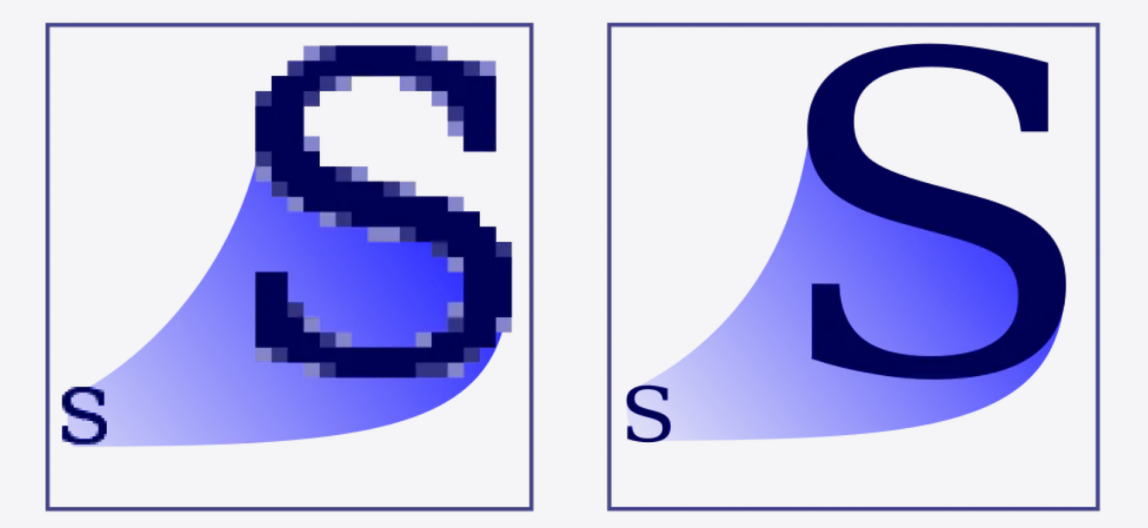
\includegraphics[width=0.6\textwidth]{figure_raster_vector.png}
    \caption{Comparaison entre une image matricielle (a) et une image vectorielle (b).}
    \label{fig:raster_vector}
\end{figure}

Afin de mieux comprendre la manière dont une image vectorielle est construite et enregistrée, il convient de présenter deux éléments essentiels. Les courbes de Bézier permettent de représenter des contours et des formes complexes à partir d'un nombre limité de points de contrôle, tandis que le format SVG fournit une structure permettant de décrire et de stocker ces primitives vectorielles.

\subsubsection{Courbes de Bézier}
\label{sec:courbes_bezier}

Une courbe de Bézier est définie comme une fonction polynomiale dont la forme est dictée par la position de points de contrôle. La courbe passe par le premier et le dernier point (points d'ancrage), tandis que les points intermédiaires agissent comme des "aimants" qui tirent la courbe vers eux \cite{foley1996computer}. 

Les courbes de Bézier font partie des formes géométriques individuelles qui composent les images vectorielles et se distinguent par le faible nombre de données numériques nécessaires à la représentation de formes complexes.
     
    \subsubsection{Format SVG}
    %ici c'est bel et bien un article et non un site web qui est cité donc je ne citerai pas la date mdr allez vous faire foutre
		SVG (Scalable Vector Graphics) est un format basé sur XML comportant des directives pour la définition de graphiques 2D\cite{w3c2011svg}. Stockées dans des fichiers textes rendant les SVG compressible et indexable, ces directives SVG supportent aussi bien les formes géométriques vectorielle que les images et le texte. Pour les raisons précédentes ce sera ce format qui sera préféré pour la sortie du modèle.
		\begin{figure}[H]
        \centering
        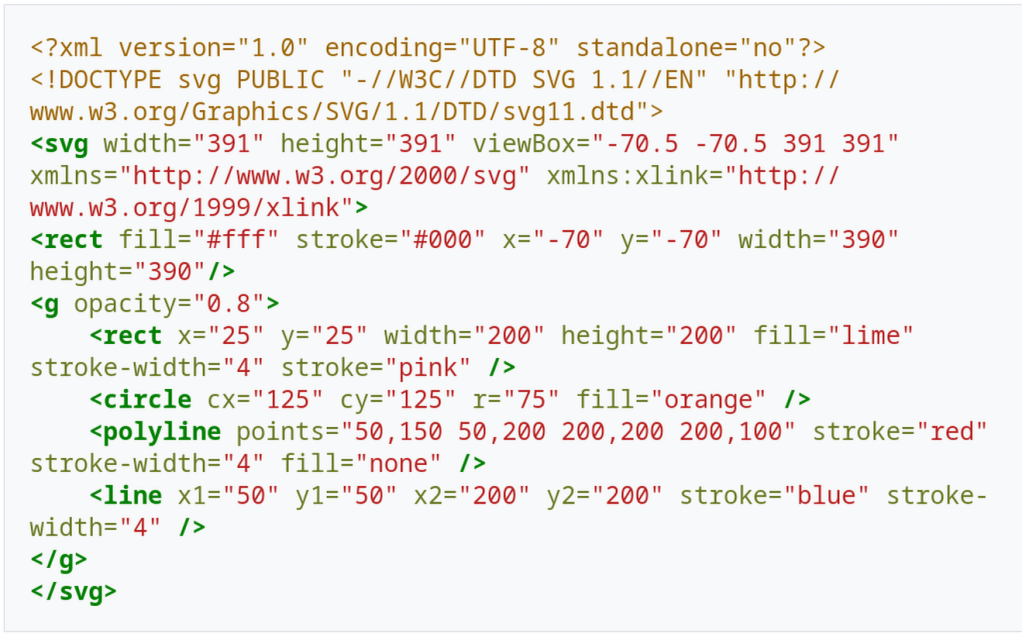
\includegraphics[width=0.6\textwidth]{figure_svg.png}
        \caption{Exemple du contenu d'un fichier .svg}
    \end{figure}
\section{Apprentissage automatique et apprentissage profond}

Cette section présente les notions d'apprentissage automatique et d'apprentissage profond nécessaires à la compréhension des approches modernes de vectorisation d'images. Elle introduit d'abord les principaux modes d'apprentissage, notamment l'apprentissage auto-supervisé, puis décrit les architectures profondes utilisées pour extraire et traiter les caractéristiques visuelles, en particulier les réseaux de neurones, les Transformers et les Vision Transformers.

\subsection{Apprentissage automatique et apprentissage auto-supervisé}
	L'apprentissage automatique est une discipline du domaine de l'intelligence artificielle dans laquelle, contrairement à l'approche programmatique classique, la machine ne reçoit pas une suite d'instructions détaillées pour résoudre une tâche donnée, car ces instructions seraient souvent trop complexes à définir explicitement \cite{geron2022hands}. Le principe consiste plutôt à apprendre à partir d'un ensemble de données afin d'améliorer progressivement une performance $P$ sur une tâche $T$ à partir d'une expérience $E$, selon la définition proposée par Mitchell \cite{mitchell1997ml}.

Selon la nature des données et du signal de supervision disponibles, plusieurs modes d'apprentissage peuvent être distingués. Dans l'apprentissage supervisé, chaque exemple d'entrée est associé à une cible ou à une étiquette attendue. À l'inverse, dans l'apprentissage non supervisé, le modèle cherche à découvrir des structures présentes dans les données, telles que des groupes d'exemples similaires ou des représentations de plus faible dimension \cite{bishop2006pattern}.

Cependant, dans le contexte de la vision par ordinateur moderne, ces deux catégories ne suffisent pas toujours à expliquer l'intérêt des modèles pré-entraînés utilisés pour l'extraction de caractéristiques visuelles. En effet, l'annotation manuelle de grands ensembles d'images est une tâche coûteuse et parfois difficile à généraliser à tous les domaines. C'est dans ce cadre que l'apprentissage auto-supervisé prend une place importante. Cette approche exploite des données non étiquetées tout en générant automatiquement un signal de supervision à partir des données elles-mêmes, par exemple en demandant au modèle de prédire une partie manquante, une transformation appliquée ou une relation entre différentes vues d'une même image \cite{jing2021selfsupervised}. Elle permet ainsi d'apprendre des représentations visuelles générales à partir de grandes collections d'images sans annotations humaines explicites, représentations qui peuvent ensuite être transférées vers d'autres tâches de vision par ordinateur \cite{geron2022hands,jing2021selfsupervised}. Dans le cadre de la vectorisation d'images, cet aspect est particulièrement pertinent, car l'objectif n'est pas seulement de classer une image, mais d'en extraire une représentation riche de sa structure, de ses régions et de ses détails visuels, afin de faciliter ensuite la prédiction de primitives vectorielles.

	\subsection{Apprentissage profond}
	L'apprentissage profond est une sous-branche de l'apprentissage automatique fondée principalement sur les réseaux de neurones profonds. Ces modèles sont constitués de plusieurs couches de neurones artificiels capables d'apprendre progressivement des représentations de plus en plus abstraites à partir des données. Cette approche s'est fortement développée grâce à l'augmentation de la puissance de calcul, à la disponibilité de grandes quantités de données et aux progrès réalisés dans l'entraînement des réseaux profonds \cite{geron2022hands}. Dans le domaine du traitement d'images, les réseaux de neurones convolutionnels (CNN) ont longtemps constitué l'une des architectures dominantes, grâce à leur capacité à exploiter la structure spatiale locale des images et à extraire automatiquement des caractéristiques visuelles telles que les contours, les formes ou les textures \cite{lecun1989backpropagation,gonzalez2018digital}. Cependant, les architectures récentes fondées sur l'attention, en particulier les Transformers et les Vision Transformers, ont progressivement élargi cette approche en permettant de modéliser des relations plus globales entre les différentes régions d'une image.
		\subsubsection{Réseaux de neurones}
		Les réseaux de neurones artificiels sont des modèles d'apprentissage automatique inspirés, de manière simplifiée, du fonctionnement des neurones biologiques. Ils sont constitués d'unités de calcul appelées neurones artificiels, organisées en couches et reliées entre elles par des connexions pondérées. L'apprentissage consiste à ajuster ces poids à partir des données d'entraînement afin que le réseau puisse produire une sortie correcte pour une tâche donnée \cite{geron2022hands}. Dans le domaine du traitement d'images, ces modèles sont utilisés pour apprendre automatiquement des fonctions de décision à partir d'exemples, notamment dans les problèmes de classification, de reconnaissance de formes et de reconstruction \cite{gonzalez2018digital}.		
\subsubsection{Transformers}

Les Transformers sont une architecture de réseaux de neurones introduite initialement pour le traitement des séquences, notamment en traduction automatique. Contrairement aux réseaux récurrents, ils ne traitent pas les éléments de la séquence de manière strictement séquentielle, mais s'appuient principalement sur des mécanismes d'attention, en particulier l'auto-attention, afin de modéliser les relations entre les différents éléments d'une entrée \cite{vaswani2017attention}. Grâce à leur capacité à apprendre des dépendances complexes et à être entraînés efficacement sur de grandes quantités de données, les Transformers ont ensuite été largement utilisés dans de nombreux domaines de l'apprentissage profond, notamment le traitement du langage naturel, la vision par ordinateur et les modèles multimodaux \cite{geron2022hands}. Comme l'illustre la figure~\ref{fig:transformer_encoder}, un encodeur Transformer peut être représenté de manière simplifiée par un mécanisme d'auto-attention multi-têtes suivi d'un réseau feed-forward.

\begin{figure}[H]
    \centering
    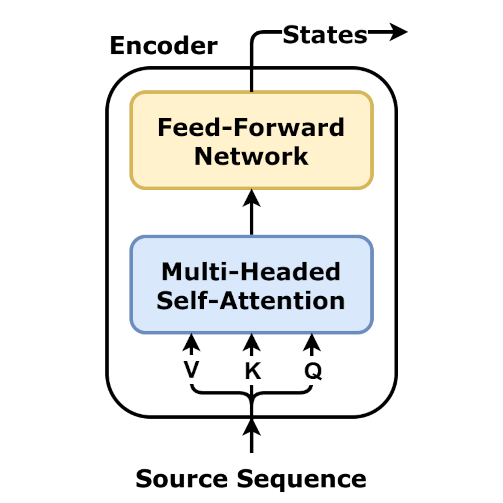
\includegraphics[width=0.38\textwidth]{transf_encself.png}
    \caption[Structure simplifiée d'un encodeur Transformer]
    {Structure simplifiée d'un encodeur Transformer. Figure adaptée de dvgodoy, sous licence CC BY 4.0.}
    \label{fig:transformer_encoder}
\end{figure}	
						
\subsubsection{Vision Transformers}
\label{sec:vision_transformers}

Les Vision Transformers, ou ViT, sont une adaptation de l'architecture Transformer au traitement des images. Au lieu de s'appuyer principalement sur des convolutions comme les CNN, une image est divisée en petits blocs appelés patchs, par exemple de taille $16 \times 16$. Ces patchs sont ensuite transformés en vecteurs et traités comme une séquence d'éléments, de manière similaire aux tokens dans le traitement du langage naturel \cite{dosovitskiy2021image}. Grâce au mécanisme d'auto-attention, le modèle peut apprendre des relations globales entre différentes régions de l'image. Cette capacité rend les Vision Transformers particulièrement intéressants pour les tâches où la compréhension de la structure globale de l'image est importante, en complément des informations locales. Comme l'illustre la figure~\ref{fig:vit_model}, les représentations des patchs sont combinées à un encodage positionnel, puis transmises à un encodeur Transformer afin de produire la sortie du modèle.

\begin{figure}[H]
    \centering
    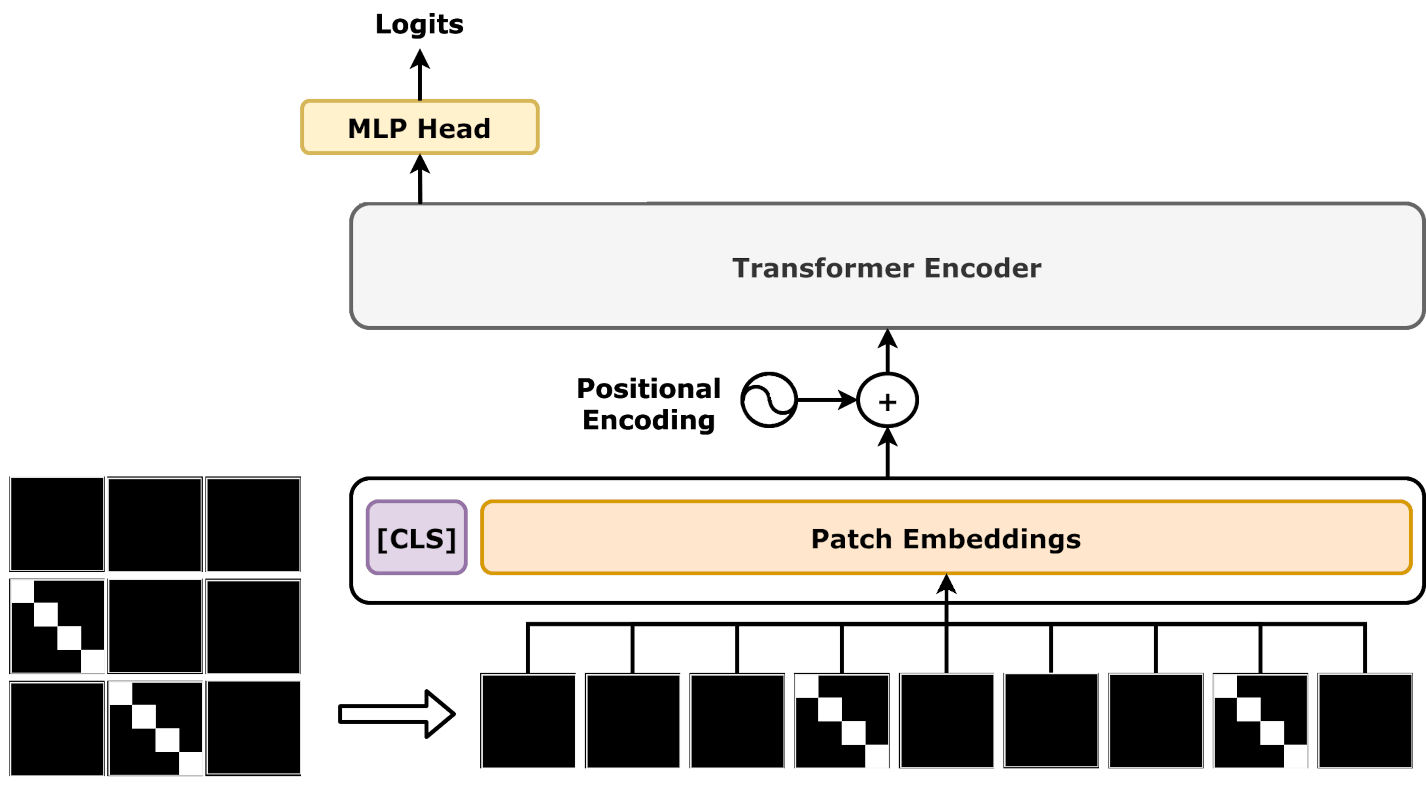
\includegraphics[width=0.75\textwidth]{vit_model.png}
    \caption[Architecture générale d'un Vision Transformer]
    {Architecture générale d'un Vision Transformer. Figure adaptée de dvgodoy, sous licence CC BY 4.0.}
    \label{fig:vit_model}
\end{figure}

\section{Mécanismes d'attention}
\label{sec:mecanismes_attention}
Les mécanismes d'attention constituent une composante importante des architectures modernes d'apprentissage profond, en particulier dans les modèles de type Transformer. Leur objectif est de permettre au modèle d'accorder une importance différente aux éléments d'une entrée selon leur pertinence pour la tâche à résoudre, au lieu de traiter toutes les informations de manière uniforme. Ce fonctionnement repose généralement sur trois éléments principaux : une requête, des clés et des valeurs. La requête représente l'information recherchée, les clés servent à mesurer la similarité avec cette requête, et les valeurs contiennent les informations à combiner \cite{vaswani2017attention}.

Dans le cas de l'attention par produit scalaire mise à l'échelle, les requêtes, les clés et les valeurs sont regroupées respectivement dans les matrices $Q$, $K$ et $V$. Les scores d'attention sont obtenus en calculant le produit entre les requêtes et les clés, puis en le normalisant par $\sqrt{d_k}$, où $d_k$ désigne la dimension des clés. Un masque peut éventuellement être appliqué, notamment lorsque l'on souhaite empêcher le modèle d'accéder à certaines positions. La fonction softmax transforme ensuite, pour chaque requête, les scores obtenus en poids positifs compris entre 0 et 1, dont la somme est égale à 1. Les scores les plus élevés reçoivent ainsi les poids les plus importants, ce qui permet au modèle d'accorder davantage d'attention aux éléments considérés comme les plus pertinents. Ces poids sont finalement utilisés pour effectuer une combinaison pondérée des valeurs \cite{vaswani2017attention,geron2022hands}. Comme l'illustre la figure~\ref{fig:scaled_dot_product_attention}, ce mécanisme enchaîne le produit scalaire entre $Q$ et $K$, la mise à l'échelle, l'application éventuelle d'un masque, la fonction softmax et la combinaison pondérée avec $V$.

\begin{figure}[H]
    \centering
    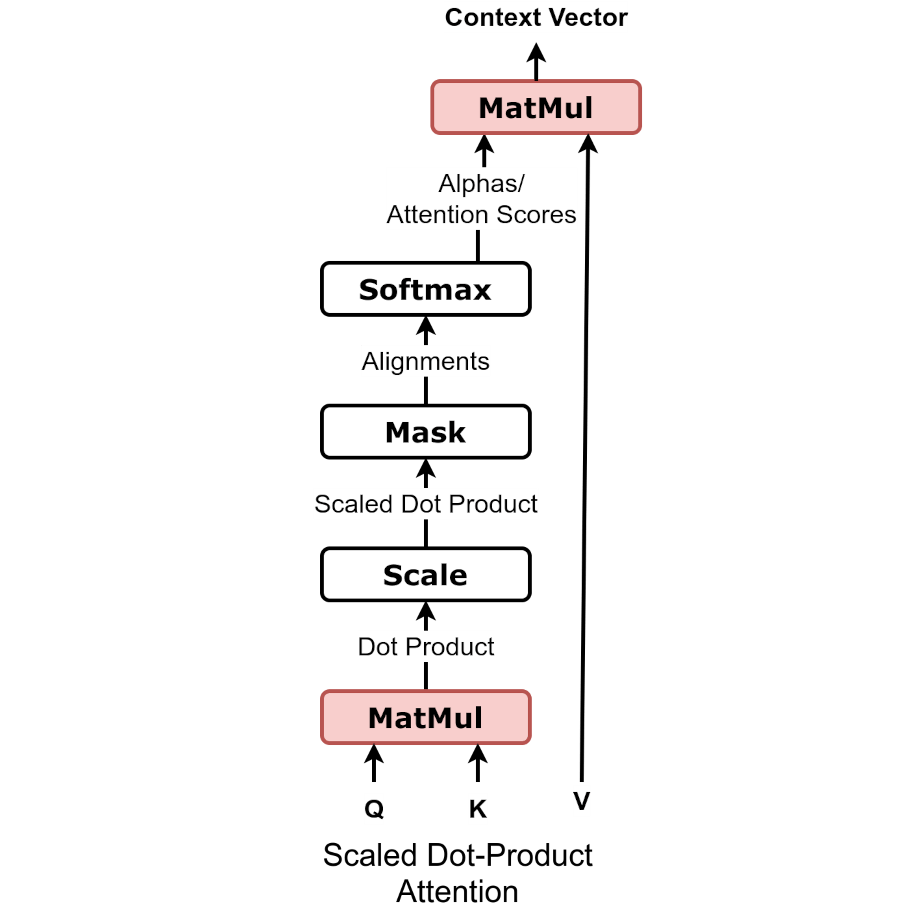
\includegraphics[width=0.55\textwidth]{aiayn_dot.png}
    \caption[Attention par produit scalaire mise à l'échelle]
    {Attention par produit scalaire mise à l'échelle. Figure adaptée de dvgodoy, sous licence CC BY 4.0.}
    \label{fig:scaled_dot_product_attention}
\end{figure}

Ce mécanisme peut être formalisé par l'équation suivante \cite{vaswani2017attention} :

\begin{equation}
    \operatorname{Attention}(Q, K, V) =
    \operatorname{softmax}\left(\frac{QK^{T}}{\sqrt{d_k}}\right)V
    \label{eq:scaled_dot_product_attention}
\end{equation}

Cette équation montre que les similarités entre les requêtes $Q$ et les clés $K$ sont transformées en poids d'attention, puis utilisées pour pondérer les valeurs $V$. Le modèle peut ainsi privilégier les informations les plus pertinentes selon le contexte, y compris lorsqu'elles sont éloignées dans la séquence ou dans l'image \cite{vaswani2017attention,geron2022hands}.

\subsection{Self-attention}
La self-attention, ou auto-attention, est un cas particulier du mécanisme d'attention dans lequel les requêtes, les clés et les valeurs proviennent de la même séquence. Elle permet donc à chaque élément d'une entrée de prendre en compte les autres éléments de cette même entrée afin de construire une représentation plus riche et contextualisée. Dans une phrase, par exemple, chaque mot peut être relié aux autres mots pour mieux comprendre son sens selon le contexte. Dans une image représentée sous forme de patchs, chaque patch peut de la même manière interagir avec les autres régions de l'image \cite{vaswani2017attention}. Cette capacité à modéliser les relations internes d'une séquence explique l'importance de la self-attention dans les architectures Transformer. Dans le traitement d'images, cette propriété permet notamment de mettre en relation des régions éloignées d'une même image, contrairement aux opérations strictement locales qui se limitent à un voisinage restreint.

\subsection{Cross-attention}
\label{sec:cross_attention}

La cross-attention, ou attention croisée, est une variante du mécanisme d'attention dans laquelle les requêtes ne proviennent pas de la même source que les clés et les valeurs. Contrairement à la self-attention, où un élément interagit avec les autres éléments d'une même séquence, la cross-attention permet à une représentation de s'appuyer sur une autre représentation externe.

Dans une architecture Transformer de type encodeur-décodeur, l'encodeur reçoit les données d'entrée et les transforme en représentations internes contenant les informations importantes de cette entrée. Le décodeur utilise ensuite ces représentations afin de générer progressivement la sortie attendue. Lors de la cross-attention, le décodeur produit les requêtes, tandis que les clés et les valeurs proviennent des représentations calculées par l'encodeur. Ce mécanisme permet ainsi au décodeur de sélectionner, à chaque étape de la génération, les informations de l'entrée les plus pertinentes \cite{vaswani2017attention,geron2022hands}.

Dans le contexte de la vectorisation d'images, l'encodeur peut extraire les caractéristiques visuelles de l'image matricielle, tandis que le décodeur génère les paramètres des primitives vectorielles. La cross-attention permet alors aux requêtes associées aux primitives à produire d'interagir avec les clés et les valeurs issues de l'image encodée. Les paramètres vectoriels prédits sont ainsi guidés par les informations visuelles les plus pertinentes, ce qui facilite la génération de primitives adaptées au contenu de l'entrée.

\section{Concepts utilisés dans la vectorisation par apprentissage profond}
\label{sec:concepts_vectorisation}
La vectorisation d'images par apprentissage profond repose sur plusieurs concepts techniques permettant de passer d'une image matricielle, composée de pixels, à une représentation vectorielle décrite par des formes paramétriques. Contrairement aux méthodes classiques de traçage, les approches récentes cherchent à apprendre ou à optimiser automatiquement les paramètres des primitives vectorielles afin de reconstruire au mieux l'image d'entrée. Pour cela, elles utilisent notamment la décomposition de l'image en régions plus simples, le rendu différentiable pour relier les paramètres vectoriels à leur rendu matriciel, ainsi que des fonctions de perte permettant de mesurer l'écart entre l'image originale et l'image reconstruite. Certaines méthodes adoptent également une stratégie progressive de type \textit{coarse-to-fine}, dans laquelle la structure globale de l'image est d'abord reconstruite avant d'ajouter les détails fins \cite{li2020diffvg,hu2024supersvg}.
    \subsection{Superpixels}
    \label{sec:superpixels}
	Les superpixels sont des régions obtenues en regroupant des pixels voisins présentant des caractéristiques similaires, notamment en termes de couleur et de position spatiale. Ils permettent de remplacer une représentation pixel par pixel par une représentation plus compacte, composée de régions visuellement cohérentes. Parmi les méthodes les plus connues, l'algorithme SLIC (\textit{Simple Linear Iterative Clustering}) adapte le principe du k-means afin de générer efficacement des superpixels. Cette méthode est appréciée pour sa simplicité, sa rapidité, sa faible consommation mémoire et sa capacité à produire des régions qui respectent bien les contours de l'image \cite{achanta2012slic}. Dans le cadre de la vectorisation d'images, les superpixels sont utiles car ils divisent une image complexe en sous-régions plus simples à traiter. SuperSVG exploite précisément cette idée en décomposant l'image d'entrée en superpixels contenant des pixels de couleurs et de textures similaires, puis en vectorisant ces régions de manière progressive \cite{hu2024supersvg}.
    \subsection{Rendu différentiable}
    \label{sec:rendu_differentiel}
	Le rendu différentiable est une technique qui permet de relier une représentation vectorielle à son rendu matriciel tout en conservant la possibilité de calculer des gradients. Dans le contexte de la vectorisation d'images, les paramètres des primitives vectorielles, comme les positions des points de contrôle, les couleurs ou l'épaisseur des traits, sont d'abord rendus sous forme d'image raster. L'image obtenue est ensuite comparée à l'image cible à l'aide d'une fonction de perte, puis les gradients de cette perte sont rétropropagés vers les paramètres vectoriels afin de les optimiser \cite{li2020diffvg}. Cette approche permet donc d'utiliser des méthodes d'optimisation ou d'apprentissage profond pour ajuster automatiquement les formes vectorielles à partir d'une supervision dans le domaine des pixels. Elle est notamment utilisée dans des méthodes comme LIVE, qui optimise progressivement des chemins de Bézier dans un cadre de rendu entièrement différentiable afin de produire des SVG organisés en couches \cite{ma2022live}.
    \subsection{Fonctions de perte}
    \label{sec:fonctions_perte_vectorisation}
	Les fonctions de perte jouent un rôle central dans la vectorisation d'images par apprentissage profond, car elles permettent de mesurer l'écart entre l'image matricielle d'origine et l'image reconstruite à partir des primitives vectorielles. Dans les approches utilisant un rendu différentiable, les chemins SVG prédits ou optimisés sont d'abord rasterisés, puis comparés à l'image cible à l'aide d'une fonction de perte calculée dans l'espace des pixels. Une perte simple, comme la MSE, peut être utilisée pour minimiser la différence entre les deux images, mais elle ne suffit pas toujours à préserver correctement la structure, les contours ou la couleur des objets. Par exemple, LIVE montre qu'une optimisation fondée uniquement sur la MSE peut conduire à un effet de couleur moyenne, puis propose une perte UDF afin de donner plus d'importance aux pixels proches des contours, ainsi qu'une perte Xing pour limiter les auto-intersections des courbes \cite{ma2022live}. Dans SuperSVG, les auteurs combinent plusieurs pertes adaptées à la vectorisation par superpixels, notamment une perte de reconstruction normalisée, une perte de frontière pour empêcher les chemins de dépasser les limites du superpixel, et une perte Dynamic Path Warping permettant au modèle de raffinement d'hériter des connaissances du modèle grossier \cite{hu2024supersvg}.
    \subsection{Apprentissage coarse-to-fine}
	L'apprentissage \textit{coarse-to-fine} désigne une stratégie progressive dans laquelle le modèle commence par reconstruire les éléments globaux ou principaux d'une image, avant d'ajouter progressivement des détails plus fins. Dans le contexte de la vectorisation d'images, cette approche est particulièrement utile car une image complexe est difficile à convertir directement en une représentation SVG précise. En procédant par étapes, le modèle peut d'abord approximer la structure générale, puis améliorer localement la reconstruction. SuperSVG adopte cette logique à travers un cadre d'apprentissage en deux étapes : un modèle grossier prédit d'abord des chemins SVG pour reconstruire la structure principale du superpixel, puis un modèle de raffinement ajoute d'autres chemins afin d'enrichir les détails, en étant guidé par les chemins prédits à l'étape précédente \cite{hu2024supersvg}. Une idée similaire apparaît dans LIVE, où l'image est reconstruite progressivement en ajoutant et en optimisant de nouveaux chemins de Bézier dans une représentation en couches, ce qui permet d'obtenir un SVG plus compact et plus cohérent avec la structure visuelle de l'image \cite{ma2022live}.
	
\section{Évaluation des résultats}

L'évaluation d'une méthode de vectorisation consiste généralement à rendre le SVG généré sous forme matricielle, puis à comparer ce rendu à l'image d'entrée. Cette section présente les principales métriques utilisées dans nos expérimentations : la MSE, le PSNR, la SSIM, la LPIPS et le temps d'inférence.

\subsection{MSE}

La MSE (\textit{Mean Squared Error}) mesure l'erreur moyenne entre les pixels de l'image originale $I$ et ceux de l'image reconstruite $\hat{I}$ :

\begin{equation}
    \operatorname{MSE}(I,\hat{I}) =
    \frac{1}{HWC}
    \sum_{i=1}^{H}
    \sum_{j=1}^{W}
    \sum_{c=1}^{C}
    \left(I_{i,j,c}-\hat{I}_{i,j,c}\right)^2
    \label{eq:mse}
\end{equation}

Dans l'équation~\eqref{eq:mse}, $H$ et $W$ représentent les dimensions de l'image et $C$ son nombre de canaux. Une valeur faible indique une reconstruction plus fidèle au niveau des pixels. Cette métrique reste toutefois limitée, car elle ne correspond pas toujours à la qualité visuelle perçue \cite{ma2022live,hu2024supersvg}.

\subsection{PSNR}

Le PSNR (\textit{Peak Signal-to-Noise Ratio}) est une métrique dérivée de la MSE. Pour des images dont les valeurs sont normalisées entre 0 et 1, il est défini par :

\begin{equation}
    \operatorname{PSNR}(I,\hat{I}) =
    10\log_{10}
    \left(
    \frac{1}{\operatorname{MSE}(I,\hat{I})}
    \right)
    \label{eq:psnr}
\end{equation}

Contrairement à la MSE, une valeur élevée du PSNR indique une meilleure fidélité de reconstruction. Cette métrique est principalement utilisée pour évaluer les différences pixel par pixel entre l'image cible et le rendu du SVG \cite{li2020diffvg,hu2024supersvg}.

\subsection{SSIM}

La SSIM (\textit{Structural Similarity Index Measure}) mesure la similarité structurelle entre deux images en prenant en compte leur luminance, leur contraste et leur structure locale \cite{wang2004ssim}. Elle est définie par :

\begin{equation}
    \operatorname{SSIM}(x,y) =
    \frac{
    (2\mu_x\mu_y+C_1)(2\sigma_{xy}+C_2)
    }{
    (\mu_x^2+\mu_y^2+C_1)
    (\sigma_x^2+\sigma_y^2+C_2)
    }
    \label{eq:ssim}
\end{equation}

Dans l'équation~\eqref{eq:ssim}, $\mu_x$ et $\mu_y$ désignent les moyennes des deux fenêtres comparées, $\sigma_x^2$ et $\sigma_y^2$ leurs variances, et $\sigma_{xy}$ leur covariance. Les constantes $C_1$ et $C_2$ assurent la stabilité du calcul. Une valeur élevée indique une meilleure préservation de la structure visuelle \cite{hu2024supersvg}.

\subsection{LPIPS}

La LPIPS (\textit{Learned Perceptual Image Patch Similarity}) compare deux images à partir de caractéristiques extraites par un réseau de neurones pré-entraîné, plutôt qu'à partir de leurs pixels uniquement \cite{zhang2018lpips}. Elle peut être exprimée sous la forme :

\begin{equation}
    \operatorname{LPIPS}(x,\hat{x}) =
    \sum_{l}
    \frac{1}{H_lW_l}
    \sum_{h,w}
    \left\|
    w_l \odot
    \left(
    \phi_l(x)_{h,w}
    -
    \phi_l(\hat{x})_{h,w}
    \right)
    \right\|_2^2
    \label{eq:lpips}
\end{equation}

Dans l'équation~\eqref{eq:lpips}, $\phi_l$ représente les caractéristiques extraites à la couche $l$ du réseau, tandis que $w_l$ désigne les poids associés à ces caractéristiques. Une faible valeur correspond à une meilleure similarité perceptuelle entre l'image d'entrée et le rendu SVG \cite{hu2024supersvg}.

\subsection{Temps d'inférence}

Le temps d'inférence correspond à la durée nécessaire pour produire un SVG à partir d'une image d'entrée. Il permet d'évaluer l'efficacité pratique d'une méthode, indépendamment de sa qualité de reconstruction. Les méthodes reposant sur l'optimisation directe des paramètres vectoriels nécessitent généralement plusieurs itérations, tandis que les modèles entraînés peuvent prédire ces paramètres plus rapidement. Cette métrique est donc utilisée conjointement avec les mesures de qualité afin de comparer la précision et la rapidité des différentes approches \cite{hu2024supersvg}.
	
\section{Travaux connexes}

La vectorisation automatique d'images a connu une évolution progressive, allant des approches algorithmiques classiques jusqu'aux travaux récents combinant apprentissage profond et rendu différentiable. Pour comparer ces travaux, il ne suffit pas de considérer uniquement la similarité visuelle entre l'image d'entrée et le SVG obtenu. Une approche de vectorisation doit également être évaluée selon plusieurs critères, notamment la fidélité visuelle, le temps de calcul, le nombre de chemins générés, la simplicité du SVG, son éditabilité, sa capacité de généralisation et le niveau de contrôle laissé à l'utilisateur \cite{dziuba2023imagevectorization}. Dans cette section, nous présentons donc les approches les plus pertinentes pour notre sujet, en montrant progressivement comment les limites des approches classiques et fondées sur l'optimisation ont conduit à des travaux plus récents comme SuperSVG.

    \subsection{Approches algorithmiques}

Les approches algorithmiques reposent généralement sur l'analyse géométrique de l'image, comme l'extraction de contours, la détection de régions ou l'ajustement de courbes. Elles sont souvent rapides et ne nécessitent pas de données d'entraînement, mais restent limitées lorsque l'image contient des couleurs complexes, des textures ou un grand nombre de détails.

        \subsubsection{Potrace}

Potrace est une méthode classique de vectorisation principalement conçue pour convertir des images binaires en contours vectoriels \cite{selinger2003potrace}. Son principe consiste à extraire les frontières entre les zones noires et blanches, à les approximer par des polygones, puis à transformer ces polygones en courbes de Bézier lisses. Cette méthode est simple, rapide et efficace pour des images comme les logos, les textes ou les dessins en noir et blanc. Cependant, elle dépend fortement de la qualité de la binarisation et reste peu adaptée aux images complexes, colorées ou texturées. Potrace constitue donc une référence importante pour les approches classiques, mais montre aussi les limites des méthodes purement algorithmiques face à une vectorisation plus générale.

    \subsection{Approches basées sur l'optimisation}

Les approches basées sur l'optimisation cherchent à ajuster directement les paramètres des primitives vectorielles afin que le rendu obtenu soit le plus proche possible de l'image d'entrée. Avec le rendu différentiable, il devient possible de calculer des gradients entre l'image rendue et l'image cible, puis de les utiliser pour modifier les courbes, les couleurs ou l'opacité des chemins SVG.

        \subsubsection{DiffVG}

DiffVG propose un rasteriseur différentiable permettant de relier le domaine vectoriel au domaine matriciel \cite{li2020diffvg}. Grâce à ce mécanisme, un ensemble de courbes ou de formes vectorielles peut être rendu sous forme d'image, comparé à une image cible, puis optimisé par rétropropagation. Cette approche est importante car elle permet d'utiliser une supervision uniquement matricielle, sans avoir besoin d'un SVG de référence. Elle est donc devenue une base technique pour plusieurs méthodes récentes. Cependant, DiffVG reste coûteux lorsqu'il faut optimiser beaucoup de chemins ou effectuer un grand nombre d'itérations. De plus, le nombre de primitives doit souvent être fixé à l'avance, ce qui limite le contrôle automatique de la complexité du SVG.

        \subsubsection{LIVE}

LIVE, pour \textit{Layer-wise Image Vectorization}, améliore les approches d'optimisation en introduisant une reconstruction progressive par couches \cite{ma2022live}. La méthode ajoute progressivement des chemins de Bézier, puis les optimise afin de reconstruire l'image de manière \textit{coarse-to-fine}. Cette stratégie permet d'obtenir des SVG plus structurés, plus compacts et plus éditables que ceux produits par une optimisation naïve. LIVE introduit également des pertes spécifiques pour mieux préserver les contours et limiter les auto-intersections des chemins. Malgré ces avantages, la méthode reste lente, car chaque image nécessite une optimisation itérative. Le résultat dépend aussi du nombre de chemins choisi et de plusieurs hyperparamètres. LIVE montre donc l'intérêt d'une représentation vectorielle progressive et éditable, mais confirme aussi le besoin de méthodes plus rapides.

    \subsection{Approches basées sur l'apprentissage profond}

Les approches basées sur l'apprentissage profond cherchent à apprendre directement la relation entre une image matricielle et une représentation vectorielle. Contrairement aux méthodes d'optimisation qui ajustent les chemins pour chaque image, ces méthodes entraînent un modèle capable de prédire les paramètres vectoriels à partir de l'image d'entrée, ce qui permet généralement une inférence plus rapide.

        \subsubsection{Im2Vec}
Im2Vec propose une méthode de génération de graphiques vectoriels sans supervision vectorielle directe \cite{reddy2021im2vec}. Contrairement aux approches qui nécessitent des fichiers SVG annotés, le modèle apprend uniquement à partir d'images matricielles. Son architecture suit un schéma encodeur-décodeur : l'image d'entrée est d'abord encodée dans un espace latent, puis ce code latent est utilisé pour générer une représentation vectorielle composée de plusieurs chemins fermés. Pour gérer les formes constituées de plusieurs composants, Im2Vec utilise un module récurrent de type RNN/LSTM qui produit un code latent propre à chaque chemin. Chaque chemin est ensuite décodé sous forme de courbes de Bézier à l'aide d'un décodeur fondé sur des convolutions 1D circulaires, ce qui permet de modéliser des formes fermées comme des déformations d'un cercle.

Le résultat vectoriel généré est ensuite rendu sous forme matricielle à l'aide d'un rendu différentiable, puis comparé à l'image cible afin d'entraîner le modèle sans supervision SVG explicite. Cette approche est intéressante car elle évite le besoin de jeux de données vectoriels annotés, qui sont difficiles à obtenir et souvent ambigus, puisqu'une même image peut être représentée par plusieurs structures vectorielles différentes. Cependant, Im2Vec reste surtout adapté à des images relativement simples ou appartenant à des domaines limités, comme les icônes, les caractères ou les emojis. Il montre donc l'intérêt de l'apprentissage profond pour la génération et la vectorisation de formes paramétriques, mais reste limité pour traiter des images complexes et variées.

        \subsubsection{SuperSVG}
SuperSVG est la méthode la plus proche de notre thématique et constitue une référence importante dans les travaux récents de vectorisation image-to-SVG \cite{hu2024supersvg}. Son principe consiste d'abord à décomposer l'image d'entrée en superpixels, afin de réduire la difficulté du problème en travaillant sur des régions plus homogènes en couleur et en texture. Chaque superpixel est ensuite vectorisé séparément par un modèle d'apprentissage profond chargé de prédire les paramètres des chemins SVG correspondants.

L'architecture de SuperSVG repose sur un modèle en deux étapes. Dans la première étape, dite coarse-stage, un encodeur Vision Transformer extrait les caractéristiques visuelles du superpixel. Ces caractéristiques sont ensuite combinées avec des requêtes apprenables associées aux chemins SVG à l'aide d'un module de cross-attention. Un module de self-attention traite ensuite les représentations intermédiaires afin de les projeter vers l'espace des paramètres vectoriels. Cette première étape permet de reconstruire la structure principale du superpixel. Dans la seconde étape, dite refinement-stage, un second modèle prend en entrée le rendu obtenu à partir des chemins grossiers ainsi que le superpixel cible, puis prédit des chemins supplémentaires destinés à enrichir les détails. Les sorties des deux étapes sont finalement combinées pour produire le SVG final.

SuperSVG combine ainsi plusieurs idées importantes des travaux précédents : le rendu différentiable hérité de DiffVG, la reconstruction progressive proche de LIVE, et la prédiction directe de chemins SVG par apprentissage profond. Cette architecture lui permet d'obtenir un meilleur compromis entre qualité de reconstruction et temps de calcul, notamment par rapport aux méthodes purement basées sur l'optimisation. Néanmoins, ses résultats dépendent encore de la qualité de la décomposition en superpixels, du nombre de chemins utilisés et de la capacité du modèle à représenter correctement les détails fins de chaque région. Malgré ces limites, SuperSVG représente l'approche la plus pertinente pour notre état de l'art, car elle illustre l'évolution récente des méthodes de vectorisation vers des solutions plus rapides, plus précises et mieux adaptées aux images complexes.

\section{Synthèse comparative des approches}

Les travaux étudiés montrent que la vectorisation automatique d'images repose sur un compromis entre plusieurs critères : la fidélité visuelle, le temps de calcul, la simplicité du SVG généré, le nombre de chemins, l'éditabilité et la capacité de généralisation. Les méthodes algorithmiques privilégient généralement la rapidité et la simplicité, mais restent limitées aux images peu complexes. Les méthodes basées sur l'optimisation offrent une meilleure flexibilité grâce au rendu différentiable, mais leur coût augmente avec le nombre de chemins et d'itérations. Les approches basées sur l'apprentissage profond cherchent à dépasser cette limite en apprenant à prédire directement les paramètres vectoriels.




\begingroup
\footnotesize
\setlength{\tabcolsep}{3pt}
\renewcommand{\arraystretch}{1.15}
\setlength{\arrayrulewidth}{0.4pt}

\begin{longtable}{
    |p{1.7cm}
    |p{2.7cm}
    |p{2.6cm}
    |p{3.0cm}
    |p{3.0cm}|
}
\caption{Synthèse comparative des principales approches de vectorisation étudiées.}
\label{tab:synthese_vectorisation}\\

\hline
\textbf{Approche} &
\textbf{Principe} &
\textbf{Points forts} &
\textbf{Limites} &
\textbf{Apport} \\
\hline
\endfirsthead

\hline
\textbf{Approche} &
\textbf{Principe} &
\textbf{Points forts} &
\textbf{Limites} &
\textbf{Apport} \\
\hline
\endhead

Potrace &
Tracé de contours binaires et approximation par courbes de Bézier. &
Rapide, simple et sans apprentissage. &
Limité aux images complexes, colorées ou texturées ; dépend de la binarisation. &
Base des approches algorithmiques classiques. \\
\hline

DiffVG &
Optimisation de primitives SVG via un rendu différentiable. &
Permet une supervision matricielle et la rétropropagation vers les paramètres SVG. &
Coûteux, sensible à l'initialisation et au nombre de chemins fixé. &
Introduit le rendu différentiable comme outil central. \\
\hline

LIVE &
Ajout progressif de chemins de Bézier selon une logique couche par couche. &
Produit des SVG plus structurés, compacts et éditables. &
Temps de calcul élevé ; dépend des chemins et des hyperparamètres. &
Montre l'intérêt d'une reconstruction progressive. \\
\hline

Im2Vec &
Prédiction de formes vectorielles à partir d'images matricielles. &
Évite la supervision SVG directe et apprend un espace latent. &
Surtout adapté aux images simples comme les icônes, caractères ou emojis. &
Introduit l'apprentissage profond pour prédire des primitives vectorielles. \\
\hline

SuperSVG &
Vectorisation par superpixels avec reconstruction \textit{coarse-to-fine}. &
Bon compromis entre qualité, vitesse et traitement d'images complexes. &
Dépend de la décomposition en superpixels et du nombre de chemins. &
Approche récente la plus proche de notre problématique. \\
\hline

\end{longtable}
\endgroup

Cette comparaison montre que SuperSVG constitue l'approche la plus complète parmi les travaux étudiés. Elle reprend le rendu différentiable introduit par DiffVG, la logique progressive mise en avant par LIVE, et l'efficacité des modèles d'apprentissage profond. Cependant, la vectorisation automatique reste confrontée à plusieurs difficultés, notamment le contrôle de la complexité du SVG, la fidélité visuelle, le temps de calcul et la généralisation à des images variées.

\section{Conclusion}

Dans ce chapitre, nous avons présenté les notions essentielles liées à la vectorisation d'images, puis étudié les principales familles de méthodes existantes. L'analyse des travaux connexes montre une évolution progressive des approches algorithmiques vers les méthodes d'optimisation différentiable, puis vers les modèles basés sur l'apprentissage profond.

La suite du mémoire présentera l'approche proposée pour répondre à cette problématique, ainsi que les choix de conception retenus pour la mise en place du système de vectorisation.

% ============================================================
%   CHAPITRE 2 — APPROCHE PROPOSÉE
% ============================================================
\chapter{Approche proposée}
\label{chap:approche_proposee}

\section{Introduction}

Le chapitre précédent a présenté les notions nécessaires à la compréhension de la vectorisation d'images ainsi que les principales familles de méthodes existantes. Nous décrivons à présent la solution mise en œuvre dans ce projet. Son objectif est de convertir une image matricielle couleur en un ensemble de chemins vectoriels fermés, représentés par des courbes de Bézier cubiques et enregistrés dans un fichier SVG. La méthode ne nécessite pas de fichiers SVG de référence pendant l'entraînement : la supervision est obtenue en rendant les chemins prédits avec DiffVG, puis en comparant le rendu à la région matricielle d'origine.

Dans ce chapitre, nous présentons d'abord la vue d'ensemble de la méthode et la préparation des données. Nous détaillons ensuite l'architecture du modèle, la représentation des primitives vectorielles, le rendu différentiable et les fonctions de perte. Enfin, nous décrivons la stratégie d'entraînement ainsi que le passage des prédictions locales au SVG de l'image complète.

\section{Vue d'ensemble de la méthode}
\label{sec:vue_ensemble_approche}

Cette section présente l'organisation générale de l'approche proposée et ses principaux principes de fonctionnement. Nous décrivons d'abord le cheminement suivi depuis la décomposition de l'image en superpixels jusqu'à la prédiction et à l'assemblage des primitives vectorielles. Nous précisons ensuite le mode de supervision, la prédiction des chemins en une seule passe et les principaux modules constituant la pipeline.

\subsection{Principe général}

\begin{figure}[H]
    \centering
    \resizebox{\textwidth}{!}{%
    \begin{tikzpicture}[
        node distance=0.55cm,
        block/.style={
            draw,
            rounded corners=2pt,
            align=center,
            minimum height=1.15cm,
            text width=2.25cm,
            inner sep=5pt,
            font=\small
        },
        data/.style={block, fill=gray!12},
        process/.style={block, fill=blue!8},
        learned/.style={block, fill=green!10},
        result/.style={block, fill=yellow!13},
        arrow/.style={-{Latex[length=2.5mm]}, thick}
    ]

        % Ligne principale
        \node[data] (image) {Image RGB\\matricielle};

        \node[process, right=of image]
            (slic) {Segmentation\\SLIC};

        \node[process, right=of slic]
            (crop) {Recadrage, masque\\et mise à l'échelle};

        \node[learned, right=of crop]
            (dino) {Encodeur\\DINOv3--ViT};

        \node[learned, right=of dino]
            (attention) {Requêtes de chemins\\et attention};

        \node[result, right=of attention]
            (params) {$P \times 27$ paramètres\\vectoriels};

        % Ligne inférieure
        \node[process, below=1.15cm of attention]
            (diffvg) {Rendu différentiable\\DiffVG};

        \node[result, left=of diffvg]
            (losses) {Pertes de reconstruction\\et de masque};

        \node[process, below=1.15cm of params]
            (mapping) {Coordonnées locales\\vers globales};

        % Bloc légèrement élargi pour éviter les retours à la ligne indésirables
        \node[
            result,
            right=of mapping,
            text width=2.60cm,
            minimum height=1.45cm,
            inner xsep=7pt
        ]
            (svg) {Assemblage et\\enregistrement\\SVG};

        % Flux principal supérieur
        \draw[arrow] (image.east) -- (slic.west);
        \draw[arrow] (slic.east) -- (crop.west);
        \draw[arrow] (crop.east) -- (dino.west);
        \draw[arrow] (dino.east) -- (attention.west);
        \draw[arrow] (attention.east) -- (params.west);

        % Bifurcation entre entraînement et export
        \coordinate (branch) at ($(params.south)+(0,-0.38cm)$);

        \draw[thick] (params.south) -- (branch);
        \fill (branch) circle (1.2pt);

        % Branche vers DiffVG : elle passe au-dessus des nœuds inférieurs
        \draw[arrow] (branch) -| (diffvg.north);

        % Branche vers les coordonnées globales
        \draw[arrow] (branch) -- (mapping.north);

        % Branche d'entraînement
        \draw[arrow] (diffvg.west) -- (losses.east);

        % Rétropropagation vers l'encodeur
        \draw[arrow] (losses.north) -- (dino.south);

        % Export SVG
        \draw[arrow] (mapping.east) -- (svg.west);

    \end{tikzpicture}%
    }

    \caption{Pipeline générale de l'approche proposée, de l'image matricielle aux chemins SVG.}
    \label{fig:pipeline_proposee}
\end{figure}

La figure~\ref{fig:pipeline_proposee} donne une vue d'ensemble du flux avant d'en détailler les différentes étapes. Le trajet supérieur est commun à l'entraînement et à l'inférence. Les deux branches inférieures montrent, d'une part, l'utilisation du rendu différentiable pour apprendre les paramètres du réseau et, d'autre part, la transformation géométrique utilisée pour construire le document vectoriel final.

La conversion directe d'une image naturelle complète vers un nombre limité de primitives vectorielles constitue un problème difficile. Une même image peut contenir de nombreux objets, couleurs, contours et détails, tandis qu'il existe plusieurs descriptions SVG capables de produire un rendu visuellement proche. Nous réduisons cette difficulté en travaillant sur des régions dont les pixels sont plus homogènes. Comme les superpixels tendent à suivre les changements de couleur et les frontières locales, chaque prédiction porte sur une forme plus simple que l'image entière. Cette décomposition a été introduite dans la section~\ref{sec:superpixels}; elle est appliquée ici avec l'algorithme SLIC \cite{achanta2012slic}.

Pour chaque région, le réseau prédit un nombre fixé $P$ de chemins. Chaque chemin est décrit par douze points bidimensionnels et une couleur RGB, soit un vecteur de $27$ paramètres. Les chemins sont ensuite rasterisés par DiffVG. Pendant l'entraînement, cette image rendue permet de calculer une erreur de reconstruction et une pénalité lorsque les formes débordent du superpixel. Pendant l'inférence, les coordonnées prédites dans le repère local du recadrage sont replacées dans le repère de l'image originale, puis l'ensemble des chemins est enregistré au format SVG.

\subsection{Caractéristiques de l'approche proposée}

L'apprentissage repose uniquement sur des images matricielles. La correspondance entre une image et un SVG n'est pas unique : deux ensembles de courbes différents peuvent produire des rendus proches. Exiger une vérité terrain vectorielle imposerait donc une structure particulière sans garantir qu'elle soit la seule représentation correcte. Le rendu différentiable permet d'éviter cette contrainte en ramenant la supervision dans l'espace des pixels, comme dans DiffVG et plusieurs méthodes étudiées au chapitre~\ref{chap:etat_art} \cite{li2020diffvg,reddy2021im2vec}.

Les primitives sont prédites en une seule passe du réseau. Contrairement à une optimisation directe qui ajuste les courbes séparément pour chaque nouvelle image, les paramètres sont ici produits par un modèle entraîné. L'inférence ne lance donc pas de descente de gradient sur les chemins. Cette organisation sépare le coût de l'apprentissage, effectué une fois, du traitement des images ultérieures. La version implémentée emploie un seul décodeur, un nombre fixe de chemins par région et deux termes de perte directement liés à la reconstruction et au respect du masque.

Le tableau~\ref{tab:modules_approche} présente les principaux modules et les données qu'ils échangent. Les dimensions indiquées correspondent à une région redimensionnée en $224 \times 224$ pixels. La dimension interne $d$ est déterminée automatiquement à partir du modèle DINOv3 chargé.

\begin{table}[H]
    \centering
    \small
    \caption{Principaux modules de la pipeline proposée.}
    \label{tab:modules_approche}
    \begin{tabular}{p{2.7cm}p{4.1cm}p{5.5cm}}
        \toprule
        \textbf{Module} & \textbf{Entrée et sortie} & \textbf{Rôle dans la pipeline} \\
        \midrule
        SLIC & Image RGB $\rightarrow$ carte d'étiquettes & Décomposer l'image en régions localement homogènes et connexes. \\
        Prétraitement & Région et masque $\rightarrow$ tenseur $3 \times 224 \times 224$ & Recadrer le superpixel, normaliser sa taille et distinguer la région de son arrière-plan. \\
        DINOv3--ViT & Région $\rightarrow 196 \times d$ tokens & Extraire une représentation visuelle dense des $14 \times 14$ patchs. \\
        Décodeur d'attention & Tokens visuels et $P$ requêtes $\rightarrow P \times d$ & Associer chaque requête de chemin aux zones pertinentes, puis modéliser les interactions entre chemins. \\
        Tête linéaire & $P \times d \rightarrow P \times 27$ & Prédire les coordonnées normalisées et la couleur de remplissage. \\
        DiffVG & Chemins vectoriels $\rightarrow$ image RGBA & Fournir un rendu différentiable pour le calcul des pertes et un aperçu matriciel à l'inférence. \\
        Export SVG & Chemins globaux $\rightarrow$ fichier SVG & Enregistrer les primitives à la résolution de l'image d'origine. \\
        \bottomrule
    \end{tabular}
\end{table}

\section{Préparation des données}
\label{sec:preparation_donnees_approche}

Cette section décrit les opérations appliquées aux images avant leur passage dans le modèle. Nous présentons d'abord le jeu de données utilisé, puis la décomposition des images en superpixels et, enfin, la construction des recadrages locaux fournis au modéle avec leur masque associé.

\subsection{Jeu de données utilisé}

L'implémentation utilise le sous-ensemble d'entraînement d'ImageNet comme source d'images naturelles \cite{deng2009imagenet}. Les fichiers sont parcourus récursivement et chargés en RGB, puis leurs valeurs entières sont converties en nombres réels dans l'intervalle $[0,1]$. Le chargeur accepte les principaux formats matriciels, notamment JPEG, PNG, BMP, WebP et TIFF. Aucune étiquette de classe ImageNet n'intervient dans l'objectif : seules les images sont exploitées pour apprendre la reconstruction de régions visuelles.

Un exemple du jeu de données ne correspond pas à une image complète. À chaque accès, l'image concernée est segmentée, l'ordre de ses superpixels est mélangé et une région non vide est choisie. Cette stratégie permet de présenter différentes régions d'une même image au cours des époques sans stocker à l'avance tous les recadrages. En cas d'image corrompue ou de région impossible à traiter, le chargeur tente jusqu'à cinq images voisines afin qu'une erreur isolée n'interrompe pas un entraînement long.

\subsection{Décomposition en superpixels}

Pour une image $I \in [0,1]^{H_0 \times W_0 \times 3}$, l'algorithme SLIC produit une carte d'étiquettes $L \in \mathbb{N}^{H_0 \times W_0}$ \cite{achanta2012slic}. Les pixels portant la même étiquette définissent un masque binaire. Le code demande $16$ régions pendant l'entraînement, avec une compacité de $10$ et un lissage gaussien de paramètre $\sigma=1$. La connectivité est imposée afin d'éviter qu'une même étiquette corresponde à plusieurs composantes éloignées. Le nombre demandé est également borné entre $2$ et $H_0W_0$ pour conserver une valeur valide sur les petites images.

Ce choix fournit un compromis entre la taille des régions et leur homogénéité. Une valeur faible du nombre de segments laisserait au réseau des régions complexes, alors qu'une valeur très élevée multiplierait le nombre de chemins nécessaires pour reconstruire une image entière. La compacité contrôle quant à elle l'équilibre entre la proximité spatiale et la similarité colorimétrique dans SLIC \cite{achanta2012slic}. Les effets de ces paramètres sur la qualité et le coût de la vectorisation seront évalués séparément dans le chapitre consacré aux expérimentations.

\subsection{Recadrage et construction de l'entrée}

Pour un superpixel donné, nous calculons la plus petite boîte englobante $(x_1,y_1,x_2,y_2)$ contenant tous ses pixels. Dans le repère de l'image, dont l'origine se situe en haut à gauche, $x$ désigne la coordonnée horizontale et $y$ la coordonnée verticale. Le couple $(x_1,y_1)$ correspond au pixel supérieur gauche inclus dans la boîte, tandis que $x_2$ et $y_2$ représentent les bornes exclusives à droite et en bas. Le recadrage s'écrit donc $I[y_1:y_2,x_1:x_2]$, avec une largeur $x_2-x_1$ et une hauteur $y_2-y_1$. L'image et le masque sont découpés selon ces mêmes limites. Le recadrage RGB est ensuite redimensionné en $224 \times 224$ par interpolation bilinéaire, tandis que le masque utilise l'interpolation du plus proche voisin afin de rester binaire. Cette différence est importante : une interpolation continue du masque créerait des valeurs intermédiaires qui rendraient ambiguë l'appartenance à la région.

Soient $Y \in [0,1]^{3 \times H \times W}$ le recadrage RGB redimensionné et $M \in \{0,1\}^{1 \times H \times W}$ son masque, avec $H=W=224$. Le tenseur fourni au réseau est défini par :

\begin{equation}
    X = Y \odot M - (1-M),
    \label{eq:entree_region}
\end{equation}

où le masque est diffusé sur les trois canaux. Les pixels appartenant au superpixel conservent ainsi leur valeur RGB, alors que les pixels extérieurs prennent la valeur $-1$. Le réseau reçoit donc à la fois l'apparence de la région et une indication explicite de sa forme. Le tenseur cible reste $Y$, mais la perte de reconstruction sera calculée uniquement là où $M=1$. Le masque est conservé séparément pour normaliser cette perte et pénaliser les débordements.

Aucune augmentation par rotation, miroir ou modification colorimétrique n'est appliquée dans la version actuelle du chargeur. La variabilité provient du contenu d'ImageNet et du choix aléatoire du superpixel.

\section{Architecture du modèle}
\label{sec:architecture_modele_propose}

Cette section décrit l'architecture chargée de transformer les caractéristiques visuelles d'un superpixel en paramètres vectoriels. Nous présentons d'abord l'extraction des représentations avec DINOv3, puis le décodage fondé sur des requêtes apprenables, la cross-attention et la self-attention. Enfin, nous détaillons la représentation adoptée pour chaque chemin vectoriel et la manière dont ses paramètres sont interprétés sous forme de courbes de Bézier cubiques.

\subsection{Extraction des caractéristiques avec DINOv3}

L'encodeur visuel utilisé est la variante \texttt{vit\_small\_patch16\_dinov3}, chargée avec des poids pré-entraînés. DINOv3 est une famille de modèles visuels pré-entraînés par apprentissage auto-supervisé et conçus pour produire des représentations denses transférables \cite{simeoni2025dinov3}. Le recours à un modèle pré-entraîné est adapté à notre problème, car la reconstruction vectorielle nécessite de reconnaître des structures locales, des contours et des relations spatiales sans disposer d'annotations SVG.

Avant l'encodage, chaque canal de $X$ est standardisé avec les moyennes $(0{,}485,0{,}456,0{,}406)$ et les écarts-types $(0{,}229,0{,}224,0{,}225)$ employés par l'implémentation. Si la taille de l'entrée diffère de $224 \times 224$, une interpolation bilinéaire la ramène à cette résolution. Comme la taille d'un patch est de $16 \times 16$, la région est divisée en une grille de $14 \times 14$, soit $196$ patchs. Ce principe de représentation d'une image comme une séquence de patchs a été présenté dans la sous-sous-section~\ref{sec:vision_transformers} du chapitre~\ref{chap:etat_art}, consacrée aux Vision Transformers \cite{dosovitskiy2021image}.

Le passage dans DINOv3 peut être résumé par :

\begin{equation}
    F = E_{\theta}(X) \in \mathbb{R}^{196 \times d},
    \label{eq:features_dinov3}
\end{equation}

où $E_{\theta}$ désigne l'encodeur visuel et $d$ sa dimension d'embedding. La sortie de l'encodeur contient également des tokens préfixes, tels que le token de classification et, selon la variante chargée, des tokens registres. Le code retire tous ces préfixes et conserve uniquement les $196$ tokens associés aux patchs. Il vérifie explicitement leur nombre afin d'éviter de transmettre au décodeur une séquence incompatible avec la résolution prévue.

Les paramètres de DINOv3 ne sont pas gelés pendant l'entraînement. L'optimiseur reçoit l'ensemble des paramètres de l'encodeur de chemins, ce qui inclut le backbone pré-entraîné, les requêtes apprenables, les blocs d'attention et la tête de sortie. Le modèle bénéficie donc de l'initialisation auto-supervisée, puis adapte ses caractéristiques à la prédiction de primitives vectorielles.

\subsection{Requêtes apprenables et cross-attention}

Le décodeur maintient $P$ vecteurs apprenables, appelés requêtes ou tokens de chemins. Ils forment une matrice initiale $S^{(0)} \in \mathbb{R}^{P \times d}$, identique pour toutes les images avant son interaction avec les caractéristiques visuelles. Chaque requête est destinée à produire un chemin, mais aucune association fixe n'est imposée entre une requête et une position de l'image. Cette association est apprise par la cross-attention.

Pour chaque tête d'attention, les requêtes proviennent des tokens de chemins, tandis que les clés et les valeurs proviennent des patchs DINOv3. En reprenant la notation introduite dans la section~\ref{sec:mecanismes_attention}, le calcul s'écrit :

\begin{align}
    Q &= \operatorname{LN}\!\left(S^{(0)}\right)W_Q, \\
    K &= \operatorname{LN}(F)W_K, \qquad
    V = \operatorname{LN}(F)W_V, \\
    A &= \operatorname{softmax}\!\left(\frac{QK^{T}}{\sqrt{d_h}}\right)V,
    \label{eq:cross_attention_approche}
\end{align}

où $d_h$ est la dimension d'une tête. Les sorties des différentes têtes sont concaténées par le module d'attention multi-têtes. Une connexion résiduelle ajoute ensuite l'information obtenue aux requêtes initiales. Le résultat traverse un réseau \textit{feed-forward} composé de deux projections linéaires, d'une activation GELU et d'une dimension cachée quatre fois supérieure à $d$. Une seconde connexion résiduelle produit les tokens contextualisés :

\begin{equation}
    S^{(1)} = S^{(0)} + \operatorname{MHA}_{\mathrm{cross}}(S^{(0)},F,F),
    \qquad
    \widetilde{S}^{(1)} = S^{(1)} + \operatorname{FFN}\!\left(\operatorname{LN}(S^{(1)})\right).
    \label{eq:bloc_cross_attention}
\end{equation}

L'implémentation demande huit têtes. Si $d$ n'est pas divisible par huit, leur nombre est automatiquement diminué jusqu'à obtenir un diviseur valide. Cette précaution permet de conserver le même code avec plusieurs variantes de backbone.

\subsection{Interactions entre les chemins}

Après la cross-attention, chaque requête contient principalement l'information visuelle utile à son propre chemin. Une couche de self-attention est ensuite appliquée entre les $P$ requêtes. Les requêtes, les clés et les valeurs proviennent alors toutes de $\widetilde{S}^{(1)}$. Cette opération permet à un chemin de tenir compte des autres chemins déjà représentés, ce qui peut limiter la redondance et répartir la reconstruction entre plusieurs primitives.

Le bloc suit la même organisation pré-normalisée que le bloc précédent : LayerNorm, attention multi-têtes, connexion résiduelle, puis réseau \textit{feed-forward} et seconde connexion résiduelle. La version actuelle emploie exactement un bloc de cross-attention et un bloc de self-attention. Elle ne contient ni décodeur récurrent, ni empilement de plusieurs étapes de raffinement.

Une normalisation finale et une couche linéaire transforment chaque token en $27$ valeurs. Une fonction sigmoïde borne toutes les sorties entre $0$ et $1$ :

\begin{equation}
    Z = \sigma\!\left(W_o\operatorname{LN}(S^{(2)}) + b_o\right)
      \in [0,1]^{P \times 27}.
    \label{eq:sortie_decodeur}
\end{equation}

Cette contrainte convient simultanément aux coordonnées normalisées et aux trois composantes de couleur. Elle évite qu'un point soit placé hors du canevas local avant l'application de la perte de masque.

\subsection{Représentation d'un chemin vectoriel}
\label{sec:representation_chemin_propose}

Pour le chemin $p$, le vecteur prédit est décomposé de la manière suivante :

\begin{equation}
    z_p = \left(x_0,y_0,\ldots,x_{11},y_{11},r_p,g_p,b_p\right).
    \label{eq:parametres_chemin}
\end{equation}

Les $24$ premières valeurs représentent douze points $P_0,\ldots,P_{11}$ dans le repère normalisé du recadrage. Les trois dernières valeurs définissent la couleur de remplissage. DiffVG interprète ces points comme quatre segments de Bézier cubiques reliés bout à bout et ferme le dernier segment sur le point initial. Les points $P_0$, $P_3$, $P_6$ et $P_9$ sont les points d'ancrage, tandis que les autres points contrôlent la tangente et la courbure, comme l'illustre la figure~\ref{fig:chemin_quatre_bezier}.

\begin{figure}[H]
    \centering
    \begin{tikzpicture}[scale=1.05,
        anchorpoint/.style={circle, fill=black, inner sep=2.2pt},
        controlpoint/.style={circle, draw=black, fill=white, inner sep=1.8pt}]
        \coordinate (p0) at (0,0);
        \coordinate (p1) at (-0.8,1.2);
        \coordinate (p2) at (0.45,2.45);
        \coordinate (p3) at (2.0,2.15);
        \coordinate (p4) at (3.15,2.05);
        \coordinate (p5) at (4.25,1.2);
        \coordinate (p6) at (4.0,0.0);
        \coordinate (p7) at (3.8,-1.1);
        \coordinate (p8) at (2.7,-1.75);
        \coordinate (p9) at (1.55,-1.45);
        \coordinate (p10) at (0.45,-1.35);
        \coordinate (p11) at (-0.75,-0.75);

        \draw[densely dashed, gray] (p0)--(p1)--(p2)--(p3);
        \draw[densely dashed, gray] (p3)--(p4)--(p5)--(p6);
        \draw[densely dashed, gray] (p6)--(p7)--(p8)--(p9);
        \draw[densely dashed, gray] (p9)--(p10)--(p11)--(p0);
        \draw[very thick, blue!65!black]
            (p0) .. controls (p1) and (p2) .. (p3)
                 .. controls (p4) and (p5) .. (p6)
                 .. controls (p7) and (p8) .. (p9)
                 .. controls (p10) and (p11) .. (p0);

        \node[anchorpoint, label={[font=\scriptsize]below left:$P_0$}] at (p0) {};
        \node[controlpoint, label={[font=\scriptsize]left:$P_1$}] at (p1) {};
        \node[controlpoint, label={[font=\scriptsize]above:$P_2$}] at (p2) {};
        \node[anchorpoint, label={[font=\scriptsize]above:$P_3$}] at (p3) {};
        \node[controlpoint, label={[font=\scriptsize]above:$P_4$}] at (p4) {};
        \node[controlpoint, label={[font=\scriptsize]right:$P_5$}] at (p5) {};
        \node[anchorpoint, label={[font=\scriptsize]right:$P_6$}] at (p6) {};
        \node[controlpoint, label={[font=\scriptsize]right:$P_7$}] at (p7) {};
        \node[controlpoint, label={[font=\scriptsize]below:$P_8$}] at (p8) {};
        \node[anchorpoint, label={[font=\scriptsize]below:$P_9$}] at (p9) {};
        \node[controlpoint, label={[font=\scriptsize]below:$P_{10}$}] at (p10) {};
        \node[controlpoint, label={[font=\scriptsize]left:$P_{11}$}] at (p11) {};

        \node[font=\scriptsize, align=left] at (6.0,0.8) {Points noirs : ancrages\\Points blancs : contrôles};
    \end{tikzpicture}
    \caption{Chemin fermé composé de quatre courbes de Bézier cubiques et de douze points prédits.}
    \label{fig:chemin_quatre_bezier}
\end{figure}

Pour quatre points consécutifs $A$, $C_1$, $C_2$ et $B$, chaque segment cubique est défini, pour $t \in [0,1]$, par :

\begin{equation}
    \mathcal{B}(t) = (1-t)^3A
    + 3(1-t)^2tC_1
    + 3(1-t)t^2C_2
    + t^3B.
    \label{eq:bezier_cubique_approche}
\end{equation}

Cette équation complète le rappel sur les courbes de Bézier de la section~\ref{sec:courbes_bezier} en précisant la structure réellement produite par le modèle. Dans le premier segment, par exemple, $A=P_0$, $C_1=P_1$, $C_2=P_2$ et $B=P_3$. Le quatrième segment part de $P_9$, utilise $P_{10}$ et $P_{11}$ comme points de contrôle, puis revient à $P_0$ pour fermer la forme.

Les primitives sont remplies avec la couleur $(r_p,g_p,b_p)$. Leur opacité est fixée à $1$ et leur largeur de contour à $0$; le modèle produit donc des surfaces colorées sans trait séparé. Le nombre de chemins $P$ est un hyperparamètre fixé avant la construction du réseau. La valeur par défaut du code est $32$, tandis qu'une configuration d'entraînement enregistrée dans le projet utilise $128$ chemins par superpixel. Aucune sortie ne prédit actuellement la visibilité, l'opacité ou un symbole d'arrêt permettant de faire varier ce nombre.

\section{Rendu différentiable et fonctions de perte}
\label{sec:rendu_pertes_approche}

Cette section présente le mécanisme utilisé pour comparer les primitives vectorielles prédites à la région matricielle cible. Nous décrivons d'abord la construction de la scène et sa rasterisation avec DiffVG, puis la perte de reconstruction calculée à l'intérieur du superpixel et la pénalité appliquée aux formes qui dépassent son masque. Enfin, nous définissons l'objectif global utilisé pour entraîner l'ensemble du réseau.

\subsection{Construction de la scène DiffVG}

Les paramètres $Z$ sont convertis en objets \texttt{Path} et \texttt{ShapeGroup} de DiffVG. Pour un canevas local de largeur $W$ et de hauteur $H$, chaque coordonnée normalisée $(x,y)$ est multipliée par $(W,H)$. Les quatre segments reçoivent chacun deux points de contrôle, le chemin est déclaré fermé et sa couleur de remplissage est obtenue à partir des trois dernières valeurs du vecteur. Le rasteriseur différentiable calcule ensuite une image RGBA avec un échantillonnage $2 \times 2$ par pixel \cite{li2020diffvg}.

Si $\mathcal{R}$ désigne ce rendu, l'image RGB employée pour la reconstruction est composée sur un fond noir :

\begin{equation}
    \widehat{Y} = \mathcal{R}_{\mathrm{RGB}}(Z)
    \odot \mathcal{R}_{\alpha}(Z).
    \label{eq:composition_rendu}
\end{equation}

La différentiabilité de $\mathcal{R}$ permet de transmettre le gradient de l'erreur pixel jusqu'aux coordonnées et aux couleurs, puis à l'ensemble du réseau. DiffVG est exécuté en précision simple, même lorsque la précision mixte est active autour du reste du modèle, afin de conserver un calcul de rendu compatible et stable.

\subsection{Perte de reconstruction normalisée}

La première composante de l'objectif mesure l'écart quadratique entre le rendu et la cible à l'intérieur du superpixel. Elle dérive de la MSE définie à l'équation~\eqref{eq:mse}, mais limite le calcul aux pixels appartenant à la région et normalise leur contribution par la surface du masque, selon le principe de reconstruction par superpixels employé dans SuperSVG \cite{hu2024supersvg}. Pour un lot de taille $B$, nous définissons :

\begin{equation}
    a_i = \frac{1}{HW}\sum_{u=1}^{H}\sum_{v=1}^{W}M_{i,u,v},
    \label{eq:ratio_surface_masque}
\end{equation}

puis :

\begin{equation}
    \mathcal{L}_{\mathrm{rec}} =
    \frac{1}{B}\sum_{i=1}^{B}
    \frac{1}{3HW\max\!\left(a_i,\frac{1}{HW}\right)}
    \sum_{c=1}^{3}\sum_{u=1}^{H}\sum_{v=1}^{W}
    M_{i,u,v}\left(\widehat{Y}_{i,c,u,v}-Y_{i,c,u,v}\right)^2.
    \label{eq:perte_reconstruction_approche}
\end{equation}

Cette formulation correspond à une MSE calculée sur les pixels utiles, indépendamment de la taille relative de la région. Sans la division par $a_i$, un superpixel occupant une faible partie du recadrage contribuerait moins à l'objectif qu'une région remplissant presque toute sa boîte. La borne inférieure $1/(HW)$ protège le calcul contre une division par zéro, même si le prétraitement vérifie déjà que le masque n'est pas vide.

\subsection{Pénalité de débordement}

La perte de reconstruction ne contraint pas les pixels extérieurs au masque, puisqu'ils sont multipliés par zéro. Un chemin pourrait donc dépasser largement la région tout en reconstruisant correctement sa partie visible à l'intérieur. Pour limiter ce comportement, les mêmes formes sont rendues une seconde fois en blanc et leur canal alpha est comparé à l'extérieur du superpixel. Cette idée est proche de la perte de frontière proposée dans SuperSVG \cite{hu2024supersvg}.

Avant le calcul, le masque est dilaté par une opération de maximum local de rayon deux pixels. Soit $\widetilde{M}_i=\mathcal{D}_2(M_i)$ ce masque dilaté et $O_i=1-\widetilde{M}_i$ la zone extérieure. Si $\widehat{A}_i$ est le canal alpha du rendu blanc, la pénalité non pondérée vaut :

\begin{equation}
    \mathcal{L}_{\mathrm{ext}} =
    \frac{1}{B}\sum_{i=1}^{B}
    \frac{\displaystyle\sum_{u,v}\widehat{A}_{i,u,v}O_{i,u,v}}
         {\displaystyle\max\!\left(1,\sum_{u,v}O_{i,u,v}\right)}.
    \label{eq:perte_debordement_approche}
\end{equation}

La dilatation crée une tolérance autour de la frontière. Elle évite de pénaliser trop fortement les pixels d'anticrénelage ou un léger décalage entre le masque redimensionné et le bord de la courbe. La normalisation par la surface extérieure rend la valeur comparable entre des masques de formes différentes.

\subsection{Fonction objective}

La fonction objectif combine les deux termes précédents :

\begin{equation}
    \mathcal{L} = \mathcal{L}_{\mathrm{rec}}
    + \lambda_{\mathrm{masque}}\mathcal{L}_{\mathrm{ext}}.
    \label{eq:objectif_global_approche}
\end{equation}

Le poids de la pénalité décroît linéairement au fil des époques. Pour une époque $e \in \{0,\ldots,E-1\}$ et $E>1$, il est défini par :

\begin{equation}
    \lambda_{\mathrm{masque}}(e)
    = 0{,}05 + (0{,}01-0{,}05)\frac{e}{E-1}.
    \label{eq:poids_masque_approche}
\end{equation}

La contrainte spatiale est ainsi plus forte au début, lorsque les formes prédites sont encore peu structurées, puis son poids diminue pour laisser davantage de place à l'ajustement des couleurs et des contours. L'objectif ne contient actuellement ni perte perceptuelle LPIPS, ni SSIM, ni terme de contrôle du nombre de chemins. Ces mesures sont utiles pour l'évaluation décrite au chapitre précédent, mais elles ne participent pas à la rétropropagation de la version entraînée.

\section{Stratégie d'entraînement}
\label{sec:entrainement_approche}

Cette section décrit le protocole utilisé pour entraîner le modèle et assurer la continuité des expériences. Nous présentons d'abord les choix d'optimisation, l'ordonnancement du taux d'apprentissage et les paramètres techniques retenus, puis le mécanisme de sauvegarde permettant de reprendre un entraînement interrompu et de restaurer automatiquement sa configuration.

\subsection{Optimisation des paramètres}

L'entraînement utilise AdamW avec un taux d'apprentissage initial de $10^{-4}$ et une décroissance de poids de $0{,}05$. Le taux d'apprentissage augmente d'abord linéairement pendant une phase de \textit{warm-up}, puis suit une décroissance cosinus jusqu'à la fin de l'entraînement. Tous les paramètres de l'encodeur de chemins sont optimisés conjointement. La graine aléatoire est appliquée à Python, NumPy, PyTorch et CUDA afin de rendre les tirages aussi reproductibles que possible.

La précision mixte automatique est activée lorsque l'entraînement s'exécute sur GPU. Un facteur d'échelle dynamique est appliqué à la perte avant la rétropropagation, puis l'optimiseur et l'ordonnanceur sont mis à jour à chaque lot. Le code permet une limitation optionnelle de la norme du gradient, mais aucune valeur n'est définie dans les configurations enregistrées; cette limitation est donc inactive pour les entraînements concernés.

Le tableau~\ref{tab:configuration_entrainement} reprend la configuration complète enregistrée pour l'entraînement à $128$ chemins. Il décrit le protocole technique, sans anticiper l'analyse des performances qui appartient au chapitre suivant.

\begin{table}[H]
    \centering
    \small
    \caption{Configuration enregistrée pour l'entraînement du modèle à 128 chemins par superpixel.}
    \label{tab:configuration_entrainement}
    \begin{tabular}{p{5.1cm}p{7.4cm}}
        \toprule
        \textbf{Paramètre} & \textbf{Valeur} \\
        \midrule
        Source des images & ImageNet, avec un maximum de $10\,000$ images \\
        Taille d'une région & $224 \times 224$ pixels \\
        Paramètres SLIC à l'entraînement & $16$ régions, compacité $10$, $\sigma=1$ \\
        Backbone & \texttt{vit\_small\_patch16\_dinov3}, poids pré-entraînés \\
        Nombre de chemins par région & $128$ \\
        Taille des lots & $16$ régions \\
        Nombre d'époques & $20$ \\
        Optimiseur & AdamW, taux $10^{-4}$, décroissance de poids $0{,}05$ \\
        Ordonnancement & \textit{Warm-up} de $4$ époques, puis décroissance cosinus \\
        Précision mixte & Activée sur CUDA \\
        Graine aléatoire & $1234$ \\
        Poids de la perte de masque & Décroissance linéaire de $0{,}05$ à $0{,}01$ \\
        \bottomrule
    \end{tabular}
\end{table}

Les valeurs du tableau~\ref{tab:configuration_entrainement} décrivent la configuration effectivement entraînée et ne sont pas présentées comme l'optimum d'une recherche exhaustive. Elles résultent des contraintes de l'architecture, du budget de calcul disponible et de la nécessité de conserver un entraînement reproductible. La limite de $10\,000$ images maintient une diversité de scènes naturelles tout en bornant la durée de l'expérience. La résolution $224 \times 224$ correspond à l'entrée utilisée par le backbone DINOv3 et produit exactement $196$ patchs de taille $16 \times 16$. Les paramètres SLIC restent identiques à ceux du prétraitement : $16$ régions réduisent la complexité locale sans multiplier excessivement les recadrages, tandis que la compacité $10$ et le lissage $\sigma=1$ favorisent des régions spatialement régulières sans effacer fortement les frontières.

La variante \texttt{vit\_small\_patch16\_dinov3} a été retenue afin d'exploiter des représentations denses pré-entraînées tout en limitant le coût de l'entraînement local. Le budget de $128$ chemins par région définit la configuration finale la plus expressive évaluée dans ce travail; il quadruple le nombre de primitives par rapport à la configuration initiale à $32$ chemins, sans modifier la structure du décodeur. Les conséquences de cette augmentation sur la fidélité, le temps de rendu et la taille du SVG sont mesurées au chapitre~\ref{chap:experimentations_resultats}. La taille de lot de $16$ régions permet quant à elle de paralléliser les recadrages tout en respectant la mémoire disponible sur le GPU utilisé.

Le taux d'apprentissage de $10^{-4}$ et la décroissance de poids de $0{,}05$ fournissent des mises à jour modérées pour l'ajustement conjoint du backbone pré-entraîné et du décodeur. Le \textit{warm-up} de quatre époques limite les variations brusques au début de cette adaptation, puis la décroissance cosinus réduit progressivement le taux jusqu'à la vingtième époque, qui correspond au budget d'entraînement retenu. La précision mixte diminue le coût mémoire des opérations compatibles, tandis que la graine $1234$ fixe les principales sources d'aléa. Enfin, la décroissance du poids de masque de $0{,}05$ à $0{,}01$ impose d'abord plus fortement le respect des frontières, puis accorde progressivement davantage d'importance à la reconstruction intérieure.

\subsection{Sauvegarde et reprise}

À la fin de chaque époque, le programme enregistre l'état du modèle, de l'optimiseur, de l'ordonnanceur et du facteur d'échelle de la précision mixte. Les arguments de l'expérience sont également conservés dans le point de contrôle et dans un fichier JSON séparé. Deux formes de sauvegarde sont produites : un fichier numéroté pour chaque époque et un fichier \texttt{latest.pt} représentant le dernier état écrit.

Cette organisation permet de reprendre un entraînement sans réinitialiser le taux d'apprentissage ni les statistiques de l'optimiseur. Lors d'une reprise, l'époque suivante est calculée à partir du numéro sauvegardé et tous les états sont restaurés. Elle permet également au programme d'inférence de reconstruire automatiquement le nombre de chemins, la taille du canevas et le nom du backbone associés au modèle chargé.

\section{Inférence et génération du SVG}
\label{sec:inference_svg_approche}

Cette section décrit le passage du modèle entraîné à la génération du fichier SVG final. Nous présentons d'abord le traitement de l'image complète et la transformation des coordonnées locales en coordonnées globales, puis l'algorithme d'inférence utilisé pour assembler les chemins prédits. Nous comparons ensuite les flux d'entraînement et d'inférence avant de préciser les limites de la version actuellement implémentée.

\subsection{Traitement de l'image complète}

Pendant l'entraînement, une seule région aléatoire est extraite de chaque image chargée. À l'inférence, l'objectif est au contraire de couvrir l'image entière. SLIC est donc appliqué une fois, puis toutes les étiquettes non vides sont parcourues. La configuration par défaut demande $64$ régions, avec la même compacité $10$ et le même $\sigma=1$. Chaque région est préparée de la même manière qu'à l'entraînement et les recadrages sont regroupés par lots de $16$ avant leur passage dans le réseau.

Le modèle retourne des coordonnées normalisées dans la boîte englobante de chaque superpixel. Pour un point prédit $(u,v) \in [0,1]^2$ et une boîte $(x_1,y_1,x_2,y_2)$, le passage au repère de l'image originale est effectué par :

\begin{equation}
    x = x_1 + (x_2-x_1)u,
    \qquad
    y = y_1 + (y_2-y_1)v.
    \label{eq:coordonnees_locales_globales}
\end{equation}

Cette transformation est appliquée aux douze points de chaque chemin, tandis que la couleur reste inchangée. Les chemins de toutes les régions sont ensuite concaténés. Si SLIC produit effectivement $R$ régions et que le modèle utilise $P$ requêtes, le SVG contient donc $R \times P$ chemins. La version actuelle ne supprime aucun chemin après la prédiction et ne fusionne pas les formes similaires.

\subsection{Algorithme d'inférence}

L'algorithme~\ref{alg:inference_svg} résume les opérations réalisées. Le rendu PNG est produit à la résolution originale pour permettre une inspection rapide. Le fichier SVG est enregistré à partir des mêmes chemins globaux, sans conversion intermédiaire en pixels.

\begin{algorithm}[H]
    \caption{Vectorisation d'une image complète et génération du SVG.}
    \label{alg:inference_svg}
    \begin{algorithmic}[1]
        \Require Image RGB $I$, modèle entraîné $f_{\theta}$, nombre de régions $R$
        \Ensure Fichier SVG et aperçu PNG
        \State $L \gets \Call{SLIC}{I,R}$
        \State $S_{\mathrm{global}} \gets \varnothing$
        \ForAll{étiquettes $k$ présentes dans $L$}
            \State $M_k \gets [L=k]$
            \State $(X_k,b_k) \gets \Call{PréparerRégion}{I,M_k}$
            \State $S_k \gets f_{\theta}(X_k)$
            \State $S_k^{g} \gets \Call{LocalVersGlobal}{S_k,b_k}$
            \State $S_{\mathrm{global}} \gets S_{\mathrm{global}} \cup S_k^{g}$
        \EndFor
        \State $\widehat{I} \gets \Call{DiffVG}{S_{\mathrm{global}},\operatorname{taille}(I)}$
        \State \Call{EnregistrerPNG}{$\widehat{I}$}
        \State \Call{EnregistrerSVG}{$S_{\mathrm{global}},\operatorname{taille}(I)$}
    \end{algorithmic}
\end{algorithm}

En pratique, les régions sont traitées par lots plutôt qu'une par une comme dans ce pseudo-code, mais cette optimisation ne change pas le résultat. Le calcul est exécuté sans gradient et peut utiliser la précision mixte sur GPU. Lorsqu'un point de contrôle est chargé, les paramètres architecturaux qu'il contient sont prioritaires, sauf si l'utilisateur fournit explicitement une valeur différente sur la ligne de commande.

\subsection{Différences entre entraînement et inférence}

Le tableau~\ref{tab:entrainement_inference} met en évidence les différences qui découlent du rôle de chaque phase. Le même prétraitement local et le même réseau sont conservés, mais la sélection des régions et l'utilisation des sorties changent.

\begin{table}[H]
    \centering
    \small
    \caption{Comparaison du flux d'entraînement et du flux d'inférence.}
    \label{tab:entrainement_inference}
    \begin{tabular}{p{3.2cm}p{4.8cm}p{4.8cm}}
        \toprule
        \textbf{Élément} & \textbf{Entraînement} & \textbf{Inférence} \\
        \midrule
        Segmentation par défaut & $16$ superpixels demandés par image & $64$ superpixels demandés par image \\
        Régions traitées & Une région aléatoire par image et par accès & Toutes les régions non vides de l'image \\
        Repère des points & Coordonnées locales normalisées & Coordonnées replacées dans l'image originale \\
        DiffVG & Produit le rendu utilisé par les pertes & Produit uniquement l'aperçu PNG \\
        Sortie vectorielle & Pas de fichier SVG dans la boucle d'apprentissage & Tous les chemins sont assemblés et enregistrés \\
        Gradient & Activé jusqu'au backbone DINOv3 & Désactivé \\
        \bottomrule
    \end{tabular}
\end{table}

\subsection{Périmètre de la version implémentée}

La méthode mise en œuvre couvre la chaîne complète, depuis une image RGB jusqu'à un fichier SVG éditable, mais certains choix délimitent son comportement. Le nombre de chemins est fixé pour toutes les régions, indépendamment de leur complexité. Une zone presque uniforme reçoit donc autant de primitives qu'une zone contenant plusieurs variations de couleur. De plus, les chemins sont toujours fermés, opaques et remplis; les traits ouverts, les contours d'épaisseur variable, les dégradés et la transparence ne sont pas représentés.

La séparation en superpixels rend le problème local plus accessible, mais elle rend également le résultat dépendant de SLIC. Une frontière mal placée peut répartir un même objet entre plusieurs recadrages. La perte de masque encourage les formes à rester dans leur région, sans toutefois appliquer un découpage géométrique strict au moment de l'export. Enfin, la version actuelle ne contient pas l'étape de raffinement, la perte de transfert entre étapes ou l'optimisation finale des courbes présentes dans la méthode SuperSVG complète \cite{hu2024supersvg}.

Ces éléments ne constituent pas des résultats expérimentaux; ils décrivent le périmètre exact du système évalué. Leur influence sur la fidélité du rendu, le nombre de chemins et le temps d'inférence devra être mesurée dans le chapitre suivant à l'aide des métriques présentées au chapitre~\ref{chap:etat_art}.

\section{Conclusion}

Dans ce chapitre, nous avons présenté l'approche proposée pour la vectorisation automatique d'images matricielles. La méthode décompose d'abord l'image avec SLIC, prépare chaque superpixel dans un repère local, puis utilise un encodeur DINOv3 et un décodeur d'attention pour prédire des chemins fermés composés de courbes de Bézier cubiques. Chaque primitive est décrite par douze points de contrôle et une couleur de remplissage.

L'apprentissage ne nécessite pas de SVG cible. DiffVG transforme les prédictions en images et permet d'optimiser une perte de reconstruction normalisée ainsi qu'une pénalité de débordement hors du masque. À l'inférence, les chemins locaux sont replacés dans le repère de l'image originale, assemblés et enregistrés directement au format SVG. Le chapitre suivant sera consacré au protocole expérimental et à l'évaluation quantitative et qualitative de cette architecture.


% ============================================================
%   CHAPITRE 3 — EXPÉRIMENTATIONS ET RÉSULTATS
% ============================================================
\chapter{Expérimentations et Résultats}
\label{chap:experimentations_resultats}

\section{Introduction}

Dans ce chapitre nous présentons d'abord l'environnement matériel et logiciel, le jeu de test et les conditions du benchmark. Après les tests de validation et l'étude de l'évolution de l'apprentissage, nous comparons quantitativement et qualitativement les quatre approches. Nous revenons ensuite sur les deux configurations de notre architecture, puis discutons les principaux enseignements et les limites de l'évaluation.

\section{Environnement expérimental}
\label{sec:environnement_experimental}

Les résultats expérimentaux dépendent à la fois des ressources de calcul et des configurations logicielles employées. Nous précisons donc le matériel utilisé avant de décrire les deux configurations de notre approche qui seront évaluées dans la suite du chapitre.

\subsection{Configuration matérielle et logicielle}

Les entraînements et les évaluations ont été exécutés localement sous Windows 11. Le calcul principal repose sur une carte graphique NVIDIA GeForce RTX 4070 SUPER disposant de $12\,282$ Mo de mémoire vidéo. Le tableau~\ref{tab:environnement_experimental} récapitule les composants utilisés. Les temps présentés dans la suite dépendent de cet environnement et ne doivent donc pas être interprétés comme des valeurs indépendantes du matériel.

\begin{table}[H]
    \centering
    \small
    \caption{Environnement matériel et logiciel utilisé pour les expérimentations.}
    \label{tab:environnement_experimental}
    \begin{tabular}{p{4.2cm}p{8.4cm}}
        \toprule
        \textbf{Élément} & \textbf{Configuration} \\
        \midrule
        Système d'exploitation & Windows 11, version $10.0.26200$, architecture 64 bits \\
        Processeur & AMD Ryzen 7 7800X3D, $8$ cœurs et $16$ processeurs logiques \\
        Mémoire vive & $31{,}1$ Go \\
        Carte graphique & NVIDIA GeForce RTX 4070 SUPER, $12\,282$ Mo, pilote $591.86$ \\
        Environnement Python & Python $3.11.15$ \\
        Calcul profond & PyTorch $2.5.1$, CUDA $12.4$, précision mixte automatique \\
        Vision et modèle & timm $1.0.27$, scikit-image $0.26.0$, Pillow $11.1.0$ \\
        Rendu et métriques & pydiffvg avec extension native CUDA, LPIPS avec backbone AlexNet \\
        \bottomrule
    \end{tabular}
\end{table}

PyTorch détecte correctement le GPU et DiffVG utilise son extension CUDA. La précision mixte est activée pour le passage dans DINOv3 et le décodeur, tandis que le rendu différentiable reste calculé en précision simple, conformément à l'implémentation décrite au chapitre~\ref{chap:approche_proposee}. Les mesures LPIPS sont calculées séparément sur le processeur et ne sont pas incluses dans le temps d'inférence.

Les dépôts de référence ont été exécutés dans des environnements Conda isolés sur la même machine et la même carte graphique. SuperSVG et Im2Vec utilisent PyTorch $2.5.1$, tandis que LIVE utilise PyTorch $2.4.1$; chaque environnement dispose de pydiffvg avec prise en charge de CUDA. Cette séparation conserve les dépendances attendues par les implémentations tout en maintenant un matériel commun pour les mesures temporelles.

\subsection{Configurations de notre approche}

Les deux checkpoints évalués utilisent le même backbone \texttt{vit\_small\_patch16\_dinov3}, une entrée locale de $224 \times 224$ pixels, SLIC avec $16$ régions demandées, ainsi que l'optimiseur AdamW. Dans les deux cas, les paramètres de DINOv3 sont ajustés pendant l'entraînement : ils ne sont pas gelés. Le backbone contient $21\,586\,944$ paramètres et fait partie de l'ensemble transmis à l'optimiseur.

Le tableau~\ref{tab:configurations_evaluees} montre toutefois que les budgets d'entraînement diffèrent. La configuration à $32$ chemins utilise $5\,000$ images pendant $10$ époques, avec une limite de $200$ lots par époque. Celle à $128$ chemins utilise $10\,000$ images pendant $20$ époques et parcourt $625$ lots par époque. Le second modèle dispose donc à la fois de davantage de primitives et de davantage d'étapes d'optimisation. Les checkpoints des dixième et vingtième époques sont respectivement retenus pour représenter les deux configurations finales. L'étude interne compare ainsi des configurations complètes et ne constitue pas une ablation isolant le seul nombre de chemins.

\begin{table}[H]
    \centering
    \small
    \caption{Configurations finales comparées pendant l'évaluation.}
    \label{tab:configurations_evaluees}
    \begin{tabular}{p{5.1cm}p{3.5cm}p{3.5cm}}
        \toprule
        \textbf{Paramètre} & \textbf{Configuration 32} & \textbf{Configuration 128} \\
        \midrule
        Chemins par superpixel & $32$ & $128$ \\
        Images d'entraînement & $5\,000$ & $10\,000$ \\
        Nombre d'époques & $10$ & $20$ \\
        Lots par époque & $200$ au maximum & $625$ \\
        Taille des lots & $16$ & $16$ \\
        Époques de \textit{warm-up} & $6$ & $4$ \\
        Paramètres du modèle & $25\,160\,091$ & $25\,196\,955$ \\
        Paramètres entraînables & $25\,160\,091$ & $25\,196\,955$ \\
        Checkpoint évalué & Époque $10$ & Époque $20$ \\
        \bottomrule
    \end{tabular}
\end{table}

L'écart de $36\,864$ paramètres entre les deux réseaux provient principalement des $96$ requêtes de chemins supplémentaires. Le coût du backbone et des blocs d'attention reste presque identique. En revanche, le nombre de primitives transmises à DiffVG est multiplié par quatre, ce qui aura une influence plus importante sur le rendu et l'export du SVG que sur le passage dans le réseau.

\section{Benchmark et conditions d'évaluation}
\label{sec:protocole_evaluation}

Le benchmark repose sur des images absentes des entraînements de notre approche et sur des conditions de rendu communes. Nous détaillons d'abord la constitution des deux sous-ensembles évalués, puis les conditions d'inférence, les métriques de fidélité et les mesures de complexité vectorielle.

\subsection{Construction du jeu de test}

Les images d'entraînement sont parcourues dans un ordre déterministe avant l'application de leur limite. Le jeu interne réunit donc $12$ fichiers situés après les $10\,000$ premiers éléments de cet ordre, ce qui le rend disjoint des deux ensembles d'entraînement. Issu d'ImageNet sans utiliser les étiquettes de classe, il contient des animaux, des personnes, des objets et des scènes présentant différents niveaux de texture \cite{deng2009imagenet}.

La comparaison entre approches retient quatre de ces images : une scène complexe, deux objets sur un fond presque uniforme, une salamandre entourée d'une texture végétale et une scène sombre peu texturée. Ce sous-ensemble rend possible l'exécution complète de LIVE. Les quatre entrées sont redimensionnées en $256 \times 256$ afin de fournir les mêmes pixels aux implémentations à canevas carré. Pour l'étude interne, les $12$ images conservent au contraire leur rapport d'aspect et leur côté le plus long mesure $256$ pixels.

L'étude interne utilise les paramètres d'entraînement de SLIC, soit $16$ régions demandées, une compacité de $10$ et $\sigma=1$. Après le contrôle de connectivité, le nombre effectif varie de $5$ à $13$, avec une moyenne de $11{,}08 \pm 2{,}39$ régions. Le nombre final de chemins dépend de ce nombre effectif et du nombre de requêtes du modèle. Dans l'exemple de la figure~\ref{fig:segmentation_slic_experimentale}, les $16$ régions demandées deviennent $5$ régions connexes; la dernière vue les représente par leur couleur moyenne.

\begin{figure}[H]
    \centering
    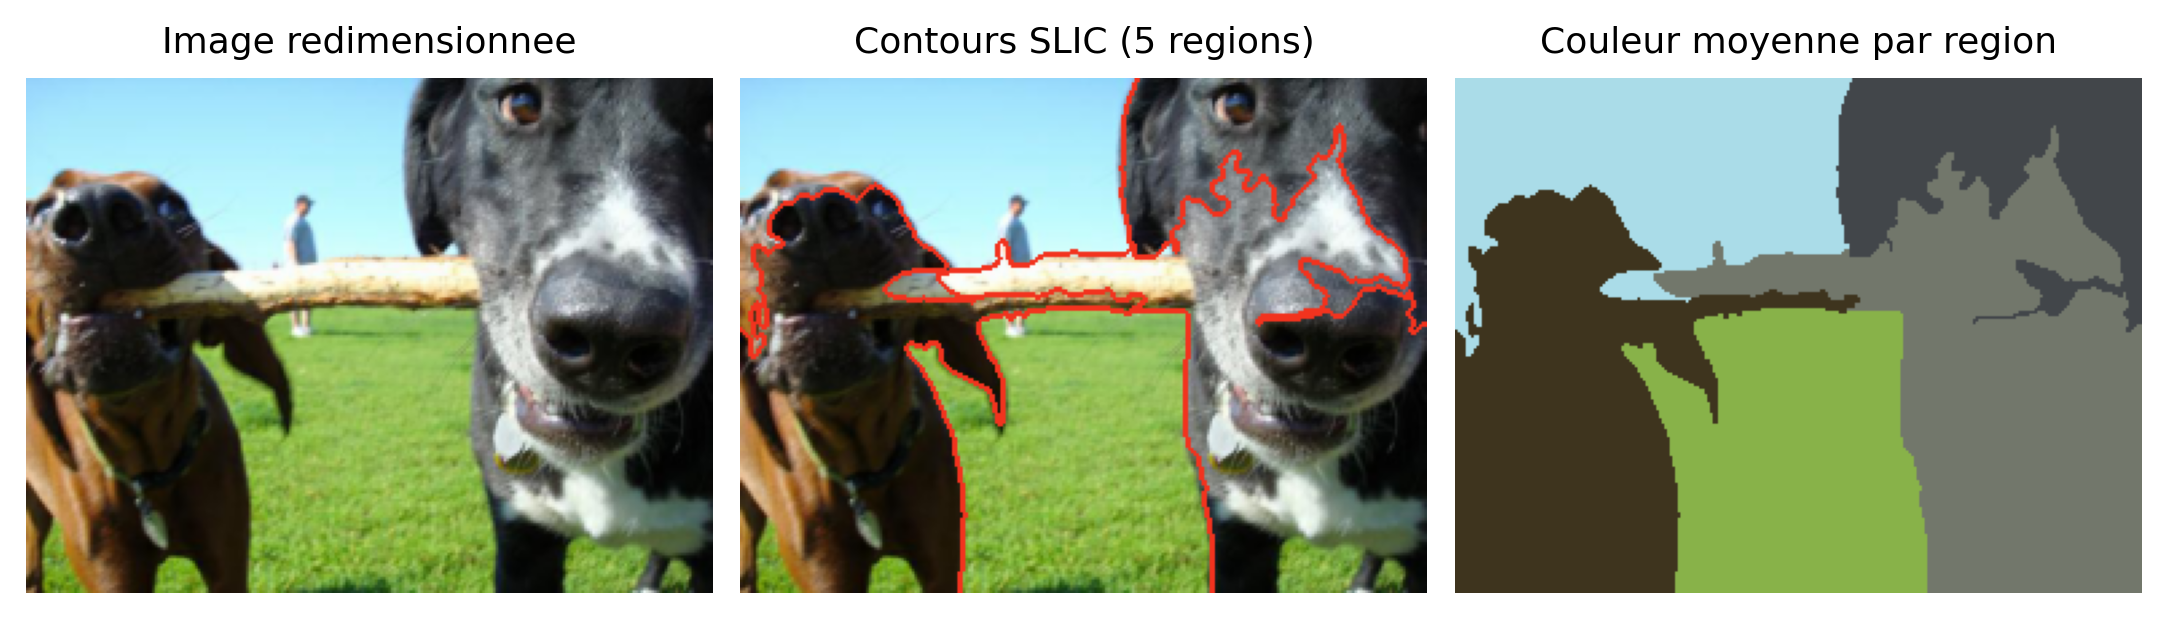
\includegraphics[width=\textwidth]{ch3_segmentation_slic.png}
    \caption{Exemple de segmentation SLIC appliquée à une image du jeu de test.}
    \label{fig:segmentation_slic_experimentale}
\end{figure}

\subsection{Conditions d'inférence}

Pour l'étude interne, les deux modèles reçoivent les mêmes images et les mêmes paramètres SLIC. Les régions sont traitées par lots de $16$ en précision mixte, puis rendues par DiffVG avec un échantillonnage $2 \times 2$ par pixel. Une phase de \textit{warm-up} précède la mesure et CUDA est synchronisé autour de chaque étape chronométrée. Le temps total additionne la préparation, la prédiction, le rendu et l'écriture du SVG; il exclut le chargement du checkpoint et de l'image, l'aperçu PNG, la validation et le calcul des métriques. Les valeurs correspondent à la moyenne des $12$ images.

Pour la comparaison externe, chaque approche produit son SVG avec les réglages de la section~\ref{sec:comparaison_methodes}. Les documents sont relus par la même version de pydiffvg, rendus avec un échantillonnage $2 \times 2$, puis ramenés à $256 \times 256$ pour les métriques. Les conventions de fond propres aux implémentations sont conservées. Le chargement des poids, la rasterisation commune et le calcul des métriques restent exclus du temps de vectorisation.

\subsection{Métriques et complexité vectorielle}

Nous utilisons les quatre métriques introduites au chapitre~\ref{chap:etat_art}. La MSE et le PSNR mesurent la fidélité au niveau des pixels, la SSIM mesure la conservation de la structure locale \cite{wang2004ssim}, et la LPIPS compare des caractéristiques perceptuelles extraites par AlexNet \cite{zhang2018lpips}. Une MSE et une LPIPS faibles sont préférables, tandis qu'un PSNR et une SSIM élevés indiquent une meilleure reconstruction. Selon l'étude, les résultats sont donnés sous la forme moyenne $\pm$ écart-type sur les $12$ images internes ou sur les quatre images communes.

La similarité matricielle ne suffit toutefois pas à caractériser un résultat vectoriel. Nous enregistrons également le nombre de chemins, le nombre de segments de Bézier cubiques, la taille du fichier SVG et le temps de vectorisation. Le nombre de segments complète le nombre de balises \texttt{path}, puisqu'un chemin peut regrouper plusieurs courbes cubiques. La taille du fichier fournit une indication pratique du coût de stockage et d'édition. Pour l'étude interne, nous conservons en plus le détail des étapes temporelles et le pic de mémoire GPU supplémentaire au-delà du modèle déjà chargé.

\section{Validation technique de l'implémentation}
\label{sec:validation_technique}

Avant l'analyse des performances, deux vérifications portent sur les mécanismes dont dépend l'évaluation. La première contrôle la transmission des gradients à travers DiffVG; la seconde vérifie l'intégrité des checkpoints, des rendus et des documents SVG produits.

\subsection{Test du rendu différentiable}

Nous avons vérifié la coopération entre PyTorch, CUDA et DiffVG en optimisant pendant $200$ étapes le centre, le rayon et la couleur d'un cercle afin de reproduire une cible. La présence et la finitude des gradients sont contrôlées pendant ce test. La MSE passe de $0{,}061617$ à $0{,}000307$ et la géométrie obtenue rejoint étroitement celle de la cible. Ce résultat ne mesure pas la qualité de la vectorisation; il vérifie la rétropropagation depuis l'image rendue vers les paramètres géométriques et colorimétriques \cite{li2020diffvg}.

\subsection{Validation des checkpoints et des SVG}

Les deux checkpoints sont chargés avec des paramètres compatibles avec leur architecture. Pour chaque image, nous contrôlons la finitude des prédictions et des pixels rendus, puis le bon format XML du SVG et sa relecture avec \texttt{pydiffvg.svg\_to\_scene}. Cette dernière vérification doit conserver les dimensions du canevas et les chemins attendus.

Le tableau~\ref{tab:validation_implementation} résume les contrôles exécutés. Les $24$ sorties correspondent aux $12$ images traitées par les deux configurations. Toutes les validations passent, ce qui confirme que les métriques sont calculées sur des rendus associés à des documents SVG effectivement rechargeables.

\begin{table}[H]
    \centering
    \small
    \caption{Résultats des tests techniques de l'implémentation.}
    \label{tab:validation_implementation}
    \begin{tabular}{p{5.5cm}p{3.2cm}p{4.0cm}}
        \toprule
        \textbf{Test} & \textbf{Résultat attendu} & \textbf{Résultat obtenu} \\
        \midrule
        Rétropropagation DiffVG sur CUDA & Gradients présents et finis & Réussi pour tous les paramètres \\
        Optimisation du cercle, $200$ étapes & Diminution de la perte & $0{,}061617 \rightarrow 0{,}000307$ \\
        Chargement strict des checkpoints & Aucun paramètre absent ou inattendu & $2/2$ checkpoints valides \\
        Finitude des sorties & Aucun NaN ou infini & $24/24$ rendus valides \\
        Analyse XML des SVG & Document bien formé & $24/24$ fichiers valides \\
        Relecture avec DiffVG & Dimensions et chemins conservés & $24/24$ scènes rechargées \\
        \bottomrule
    \end{tabular}
\end{table}

\section{Évolution de l'apprentissage}
\label{sec:evolution_apprentissage_resultats}

Les journaux détaillés de chaque lot n'ayant pas été conservés sous une forme structurée, nous ne reconstruisons pas artificiellement une courbe de perte d'entraînement. Nous évaluons plutôt cinq checkpoints cohérents de la configuration à $32$ chemins sur le même jeu de test. Les époques $1$, $3$, $5$, $7$ et $10$ sont ainsi comparées avec exactement les mêmes conditions.

\begin{table}[H]
    \centering
    \small
    \caption{Évolution des métriques moyennes du modèle à 32 chemins.}
    \label{tab:progression_32_chemins}
    \begin{tabular}{ccccc}
        \toprule
        \textbf{Époque} & \textbf{MSE $\downarrow$} & \textbf{PSNR $\uparrow$} & \textbf{SSIM $\uparrow$} & \textbf{LPIPS $\downarrow$} \\
        \midrule
        $1$  & $0{,}05351$ & $13{,}49$ & $0{,}311$ & $0{,}663$ \\
        $3$  & $0{,}03173$ & $15{,}78$ & $0{,}359$ & $0{,}618$ \\
        $5$  & $0{,}02364$ & $17{,}19$ & $0{,}368$ & $0{,}563$ \\
        $7$  & $0{,}01961$ & $18{,}14$ & $0{,}408$ & $0{,}530$ \\
        $10$ & $0{,}01615$ & $19{,}13$ & $0{,}438$ & $0{,}492$ \\
        \bottomrule
    \end{tabular}
\end{table}

La figure~\ref{fig:progression_entrainement_32} met en évidence une amélioration monotone des quatre métriques mesurées. Entre la première et la dixième époque, la MSE passe de $0{,}05351$ à $0{,}01615$, soit une diminution absolue de $0{,}03736$, tandis que le PSNR gagne $5{,}64$ dB. La SSIM passe de $0{,}311$ à $0{,}438$, soit une augmentation de $0{,}127$, et la LPIPS diminue de $0{,}663$ à $0{,}492$, soit un écart favorable de $0{,}171$. La baisse la plus forte de la MSE apparaît pendant les premières époques, puis les gains deviennent plus progressifs. Cette évolution est cohérente avec un apprentissage effectif de la reconstruction par les requêtes de chemins.

\begin{figure}[H]
    \centering
    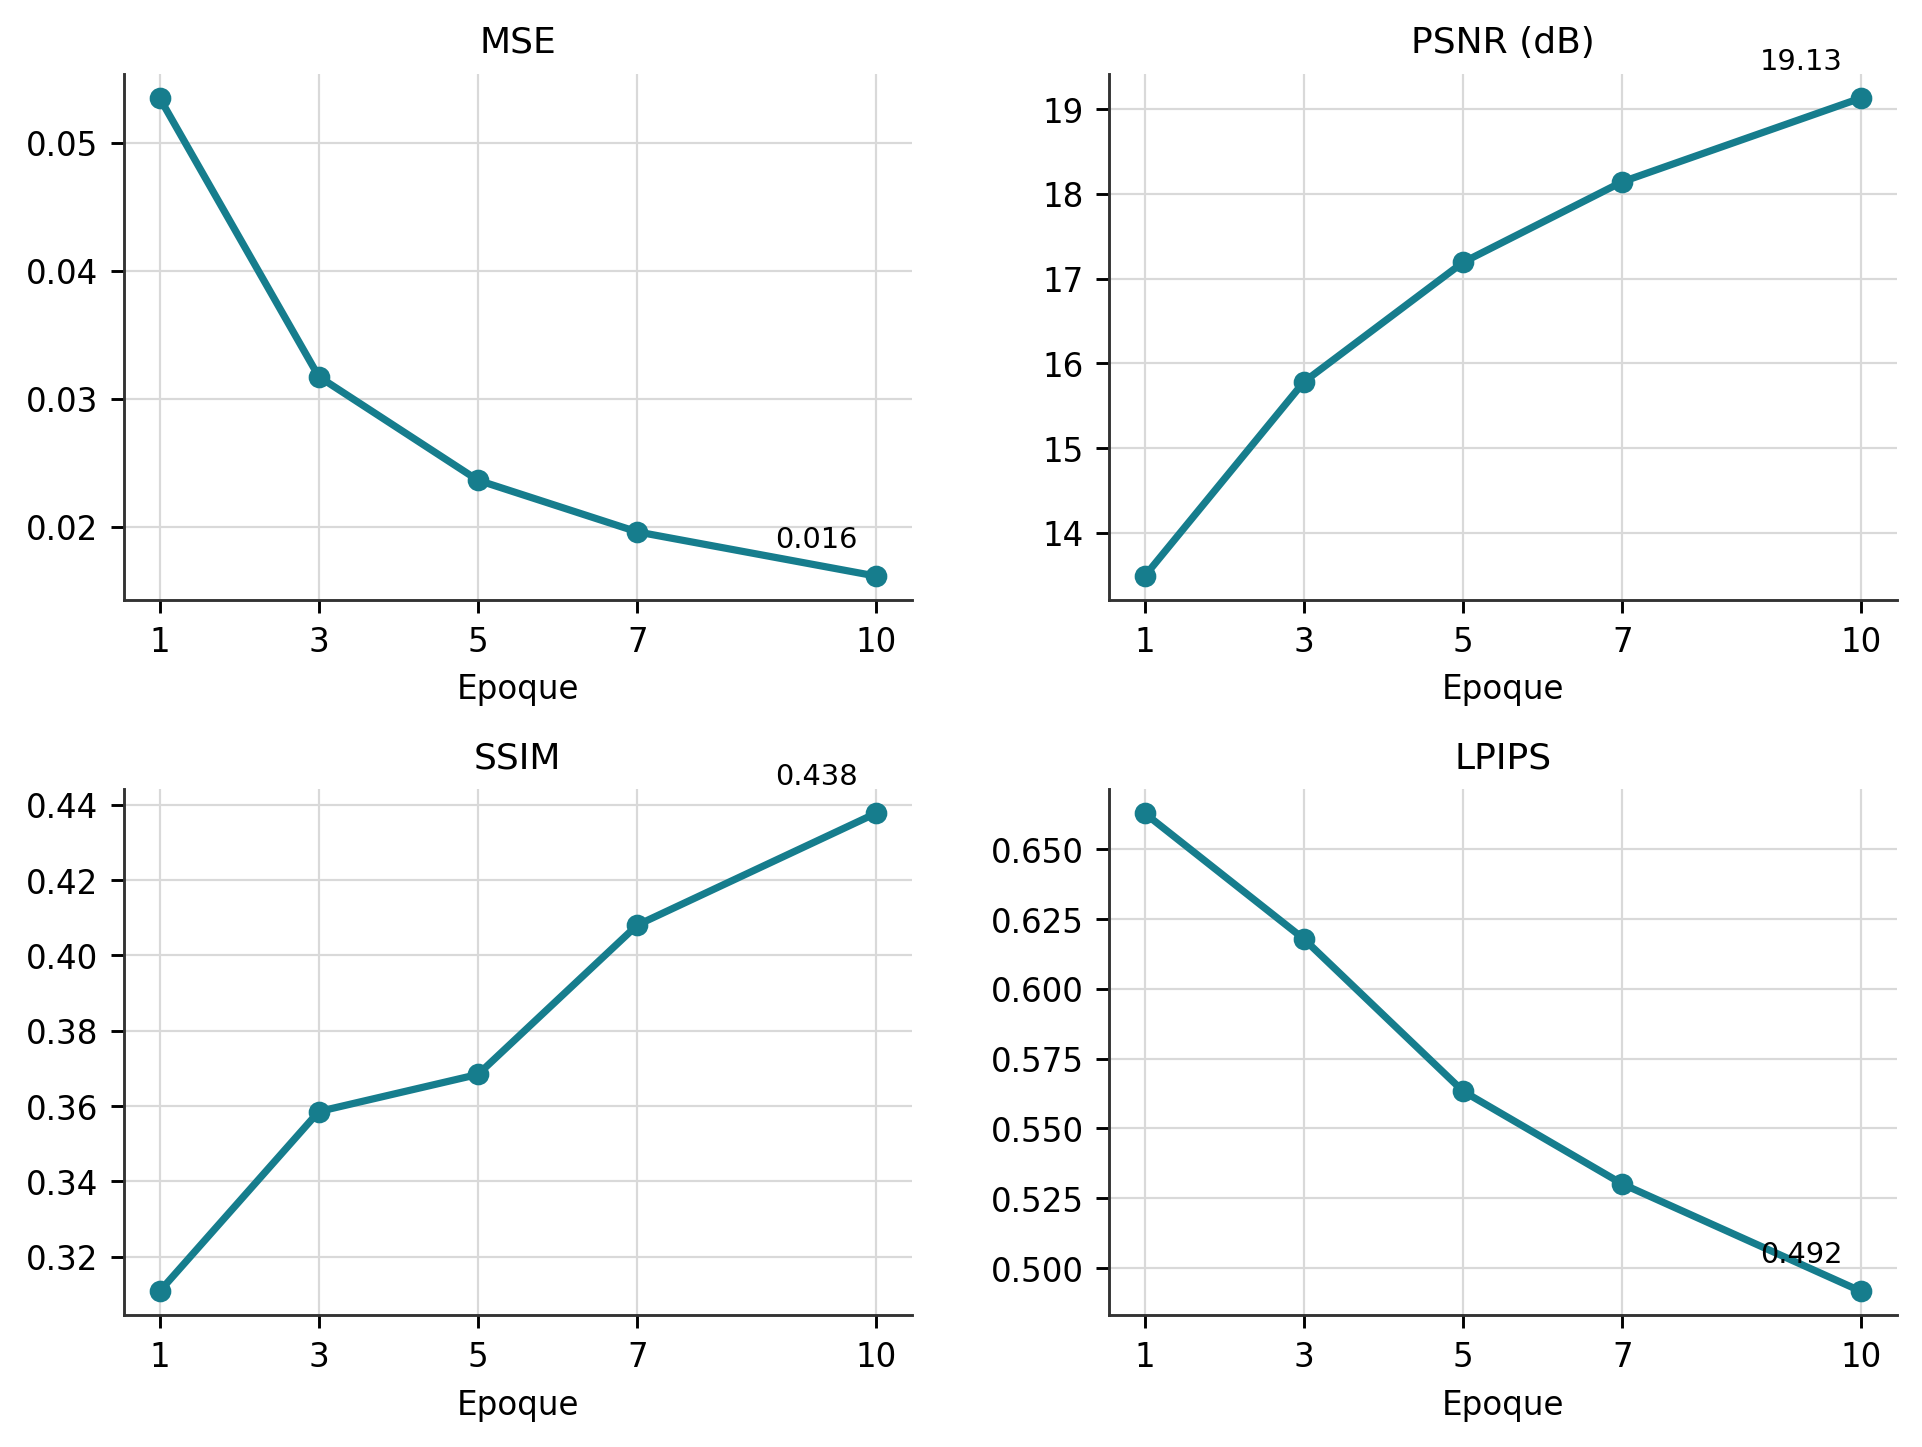
\includegraphics[width=0.92\textwidth]{ch3_progression_entrainement.png}
    \caption{Évolution des métriques sur le jeu de test pour la configuration à 32 chemins.}
    \label{fig:progression_entrainement_32}
\end{figure}

Ces valeurs ne permettent pas d'affirmer que l'entraînement est totalement convergé à l'époque $10$. Les métriques continuent à progresser entre les deux derniers points observés. Elles montrent néanmoins une trajectoire régulière sur des images non utilisées pour l'optimisation et fournissent une validation rétrospective de l'apprentissage.

\section{Comparaison avec les approches de référence}
\label{sec:comparaison_methodes}

La comparaison externe situe notre système par rapport à trois approches représentatives des travaux connexes. Nous précisons leurs configurations avant d'examiner la fidélité, le temps de vectorisation, la complexité des SVG et les différences visibles, puis nous délimitons la portée de ce benchmark.

\subsection{Configurations retenues}

Nous comparons notre modèle final à SuperSVG, LIVE et Im2Vec, présentés dans les travaux connexes du chapitre~\ref{chap:etat_art}. Les trois dépôts de référence ont été exécutés localement et aucun score publié dans les articles n'est recopié dans nos tableaux. Chaque valeur provient ainsi des mêmes quatre images et de la même procédure de rasterisation. Les configurations retenues sont résumées dans le tableau~\ref{tab:configurations_methodes_reference}.

Notre approche utilise le checkpoint de la vingtième époque, $128$ requêtes par superpixel et $16$ régions SLIC demandées. SuperSVG est chargé avec ses poids pré-entraînés grossiers et de raffinement; le nombre cible est fixé à $1\,000$ chemins et l'optimisation finale optionnelle est désactivée. Cette configuration mesure donc la prédiction \textit{coarse-to-fine} du modèle sans descente de gradient supplémentaire sur chaque image \cite{hu2024supersvg}. LIVE utilise l'expérience progressive à $32$ chemins. Les groupes $1$, $2$, $4$, $8$, $16$ puis $1$ sont ajoutés successivement, avec $500$ itérations par étape, soit $3\,000$ étapes d'optimisation par image \cite{ma2022live}.

Le checkpoint Im2Vec disponible dans le projet a été entraîné sur des emojis. Il produit quatre chemins superposés, chacun composé de vingt segments cubiques, à partir d'une entrée interne de $128 \times 128$ pixels \cite{reddy2021im2vec}. Nous l'incluons afin d'observer le comportement réel de cette représentation compacte hors de son domaine; ses résultats sur des photographies ImageNet ne représentent donc pas ceux d'un modèle Im2Vec réentraîné sur des images naturelles.

\begin{table}[H]
    \centering
    \footnotesize
    \caption{Configurations utilisées pour la comparaison entre approches.}
    \label{tab:configurations_methodes_reference}
    \begin{tabular}{p{2.2cm}p{3.4cm}p{4.0cm}p{3.4cm}}
        \toprule
        \textbf{Approche} & \textbf{Mode de vectorisation} & \textbf{Configuration évaluée} & \textbf{Budget vectoriel} \\
        \midrule
        Notre approche & Prédiction directe par superpixels & Modèle final, $16$ régions SLIC demandées, $128$ requêtes par région & Variable selon les régions effectives \\
        SuperSVG & Prédiction \textit{coarse-to-fine} & Poids officiels, cible de $1\,000$ chemins, aucune optimisation finale & $1\,000$ chemins \\
        LIVE & Optimisation différentiable par image & Calendrier $[1,2,4,8,16,1]$, $500$ itérations par étape & $32$ chemins \\
        Im2Vec & Encodage et décodage de formes latentes & Checkpoint emoji, entrée interne $128 \times 128$ & $4$ chemins de $20$ segments \\
        \bottomrule
    \end{tabular}
\end{table}

\subsection{Résultats quantitatifs communs}

Le tableau~\ref{tab:comparaison_methodes_fidelite} présente les résultats obtenus après relecture des SVG par le rasteriseur commun. SuperSVG obtient la meilleure moyenne pour les quatre métriques et se classe également premier sur chacune des quatre images prises séparément. Entre notre approche et SuperSVG, la MSE passe de $0{,}00760$ à $0{,}00151$, soit une diminution absolue favorable de $0{,}00609$, tandis que le PSNR gagne $6{,}55$ dB. La SSIM passe de $0{,}648$ à $0{,}831$, soit une augmentation de $0{,}183$, et la LPIPS diminue de $0{,}311$ à $0{,}152$, soit un écart favorable de $0{,}159$.

\begin{table}[H]
    \centering
    \small
    \caption{Comparaison de la fidélité des approches sur les quatre images communes.}
    \label{tab:comparaison_methodes_fidelite}
    \begin{tabular}{lcccc}
        \toprule
        \textbf{Approche} & \textbf{MSE $\downarrow$} & \textbf{PSNR $\uparrow$} & \textbf{SSIM $\uparrow$} & \textbf{LPIPS $\downarrow$} \\
        \midrule
        Notre approche & $0{,}00760 \pm 0{,}00779$ & $23{,}31 \pm 5{,}28$ & $0{,}648 \pm 0{,}190$ & $0{,}311 \pm 0{,}113$ \\
        SuperSVG & $\mathbf{0{,}00151 \pm 0{,}00144}$ & $\mathbf{29{,}86 \pm 4{,}44}$ & $\mathbf{0{,}831 \pm 0{,}096}$ & $\mathbf{0{,}152 \pm 0{,}066}$ \\
        LIVE & $0{,}00658 \pm 0{,}00597$ & $23{,}91 \pm 5{,}33$ & $0{,}632 \pm 0{,}223$ & $0{,}365 \pm 0{,}153$ \\
        Im2Vec & $0{,}32384 \pm 0{,}13519$ & $5{,}21 \pm 1{,}98$ & $0{,}253 \pm 0{,}189$ & $0{,}851 \pm 0{,}053$ \\
        \bottomrule
    \end{tabular}
\end{table}

\begin{figure}[H]
    \centering
    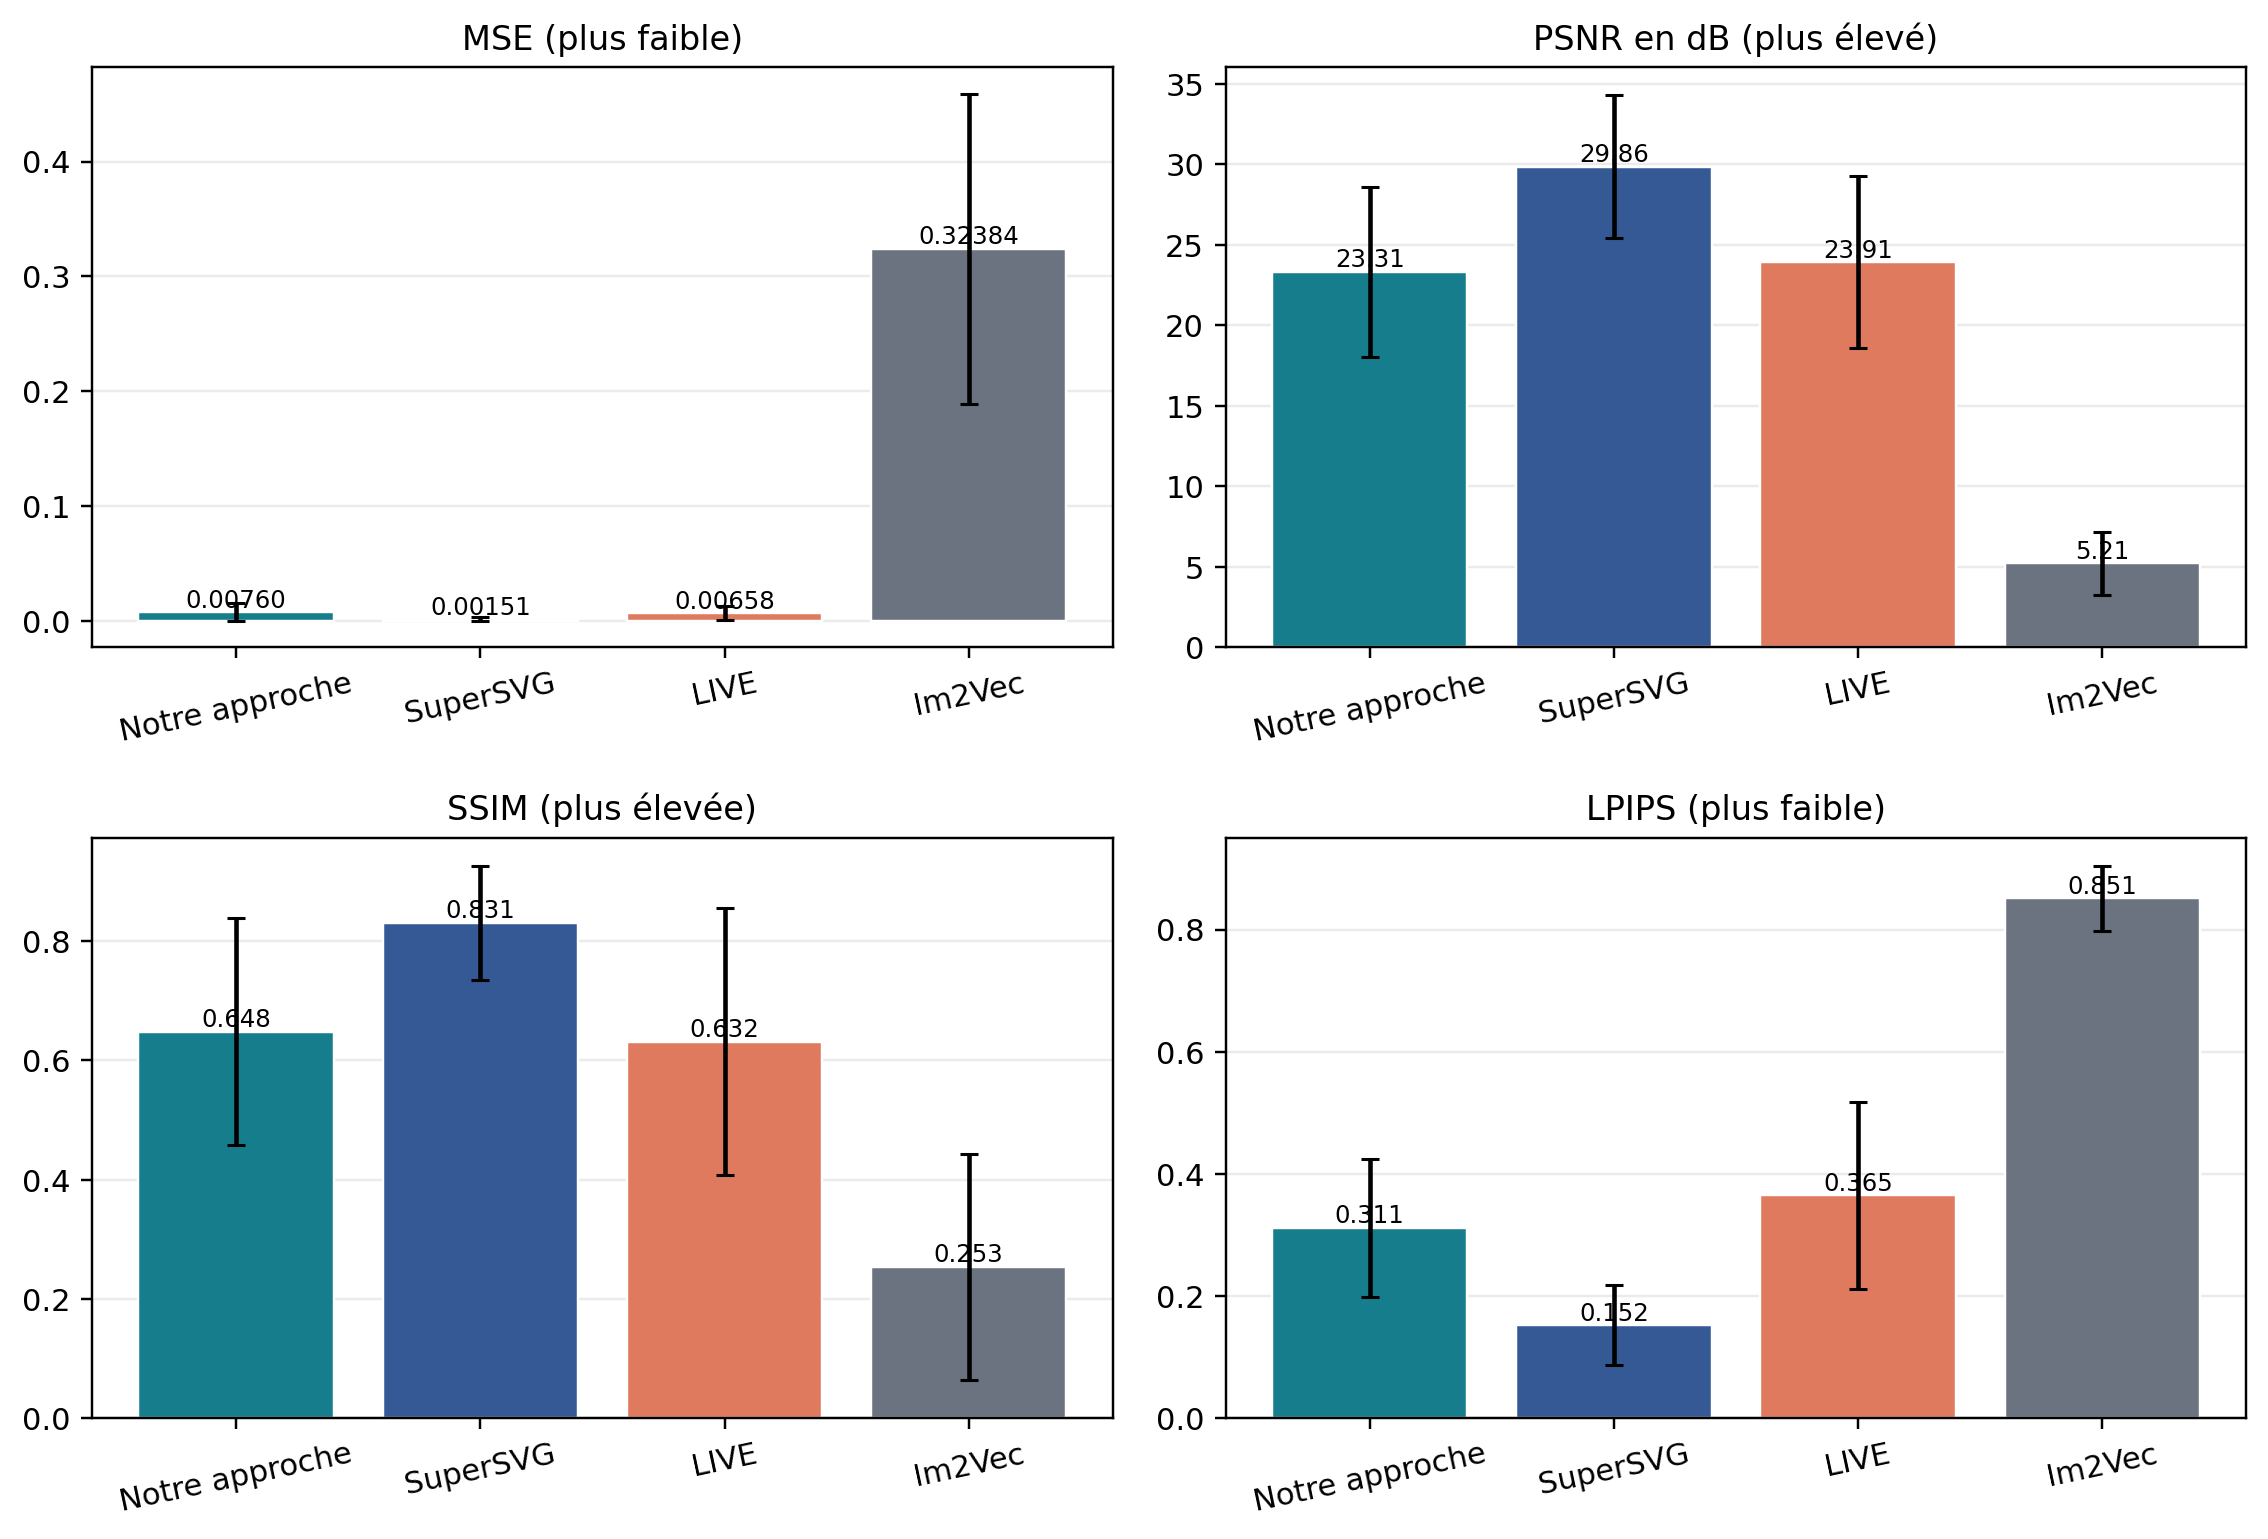
\includegraphics[width=0.98\textwidth]{ch3_comparaison_methodes_quantitative.png}
    \caption{Comparaison des quatre métriques de fidélité; les barres d'erreur représentent l'écart-type entre les images.}
    \label{fig:comparaison_methodes_quantitative}
\end{figure}

Notre approche et LIVE présentent des moyennes plus proches, mais leur classement dépend de la métrique. Entre notre approche et LIVE, la MSE passe de $0{,}00760$ à $0{,}00658$, soit une diminution favorable de $0{,}00102$, et le PSNR gagne $0{,}60$ dB. Notre modèle conserve en revanche une SSIM de $0{,}648$ contre $0{,}632$, soit un avantage absolu de $0{,}016$, ainsi qu'une LPIPS de $0{,}311$ contre $0{,}365$, inférieure de $0{,}054$. Au niveau des images individuelles, notre approche dépasse LIVE sur trois images sur quatre pour la SSIM et la LPIPS, tandis que chaque approche obtient la meilleure MSE sur deux images. Les mesures pixel par pixel favorisent donc légèrement LIVE en moyenne, alors que les mesures structurelle et perceptuelle favorisent notre modèle.

Le retrait d'Im2Vec doit être interprété au regard du décalage de domaine du checkpoint décrit précédemment. Les valeurs observées caractérisent ce modèle disponible hors de son domaine d'entraînement et ne permettent pas de conclure sur une architecture Im2Vec adaptée aux photographies.

La supériorité de SuperSVG est cohérente avec sa conception dédiée à la vectorisation par superpixels et avec son étape de raffinement, absente de notre version. Elle peut également dépendre du volume et de la stratégie d'entraînement de ses poids pré-entraînés. Comme ces facteurs ne sont pas isolés dans l'expérience, les résultats caractérisent les systèmes complets disponibles plutôt que l'apport causal d'un module particulier.

\subsection{Temps et complexité vectorielle}

Le tableau~\ref{tab:comparaison_methodes_complexite} montre que le classement de fidélité ne reflète pas directement le coût de production ou d'édition du SVG. Notre approche traite une image en $0{,}684$ seconde en moyenne, contre $2{,}548$ secondes pour SuperSVG. Elle est donc environ $3{,}72$ fois plus rapide dans cet environnement, mais produit davantage de primitives : $1\,472$ chemins et $5\,888$ segments cubiques en moyenne, contre respectivement $1\,000$ et $4\,000$ pour SuperSVG.

Im2Vec est exclu de cette comparaison temporelle. Son checkpoint ne produit que quatre chemins et ses reconstructions des photographies du benchmark ne sont pas exploitables pour la tâche étudiée. Comparer directement sa vitesse à celle des trois approches qui reconstruisent effectivement le contenu reviendrait donc à opposer des charges vectorielles et des niveaux de fidélité sans rapport. Im2Vec reste néanmoins présent dans l'analyse quantitative et qualitative précédente afin de documenter ce comportement hors domaine.

\begin{table}[H]
    \centering
    \footnotesize
    \caption{Temps et complexité des SVG produits sur les quatre images communes.}
    \label{tab:comparaison_methodes_complexite}
    \begin{tabular}{lcccc}
        \toprule
        \textbf{Approche} & \textbf{Temps (s) $\downarrow$} & \textbf{Chemins $\downarrow$} & \textbf{Segments cubiques $\downarrow$} & \textbf{SVG (Ko) $\downarrow$} \\
        \midrule
        Notre approche & $0{,}684 \pm 0{,}119$ & $1\,472 \pm 222$ & $5\,888 \pm 887$ & $662{,}10 \pm 102{,}30$ \\
        SuperSVG & $2{,}548 \pm 0{,}059$ & $1\,000 \pm 0$ & $4\,000 \pm 0$ & $544{,}04 \pm 1{,}50$ \\
        LIVE & $243{,}804 \pm 10{,}256$ & $32 \pm 0$ & $128 \pm 0$ & $21{,}01 \pm 0{,}02$ \\
        \bottomrule
    \end{tabular}
\end{table}

LIVE produit un document beaucoup plus compact, mais son optimisation progressive demande $243{,}804$ secondes par image en moyenne, soit environ quatre minutes. Notre approche est ainsi approximativement $356$ fois plus rapide. Dans les conditions du benchmark, cet écart met en évidence l'intérêt opérationnel d'une prédiction amortie : le coût de l'apprentissage est payé en amont, puis chaque nouvelle image est traitée en une passe, tandis que LIVE recommence une optimisation de $3\,000$ étapes pour chaque entrée \cite{ma2022live}. En contrepartie, les $32$ chemins de LIVE sont nettement plus faciles à parcourir et à modifier manuellement que les milliers de chemins produits par les approches à superpixels.

La figure~\ref{fig:compromis_methodes} réunit ces compromis sur des axes logarithmiques. La position de SuperSVG traduit la meilleure fidélité avec une complexité élevée, celle de LIVE une forte compacité au prix du temps, et celle de notre approche un équilibre intermédiaire entre vitesse et qualité. La taille des marqueurs dépend de la taille moyenne du fichier SVG.

\begin{figure}[H]
    \centering
    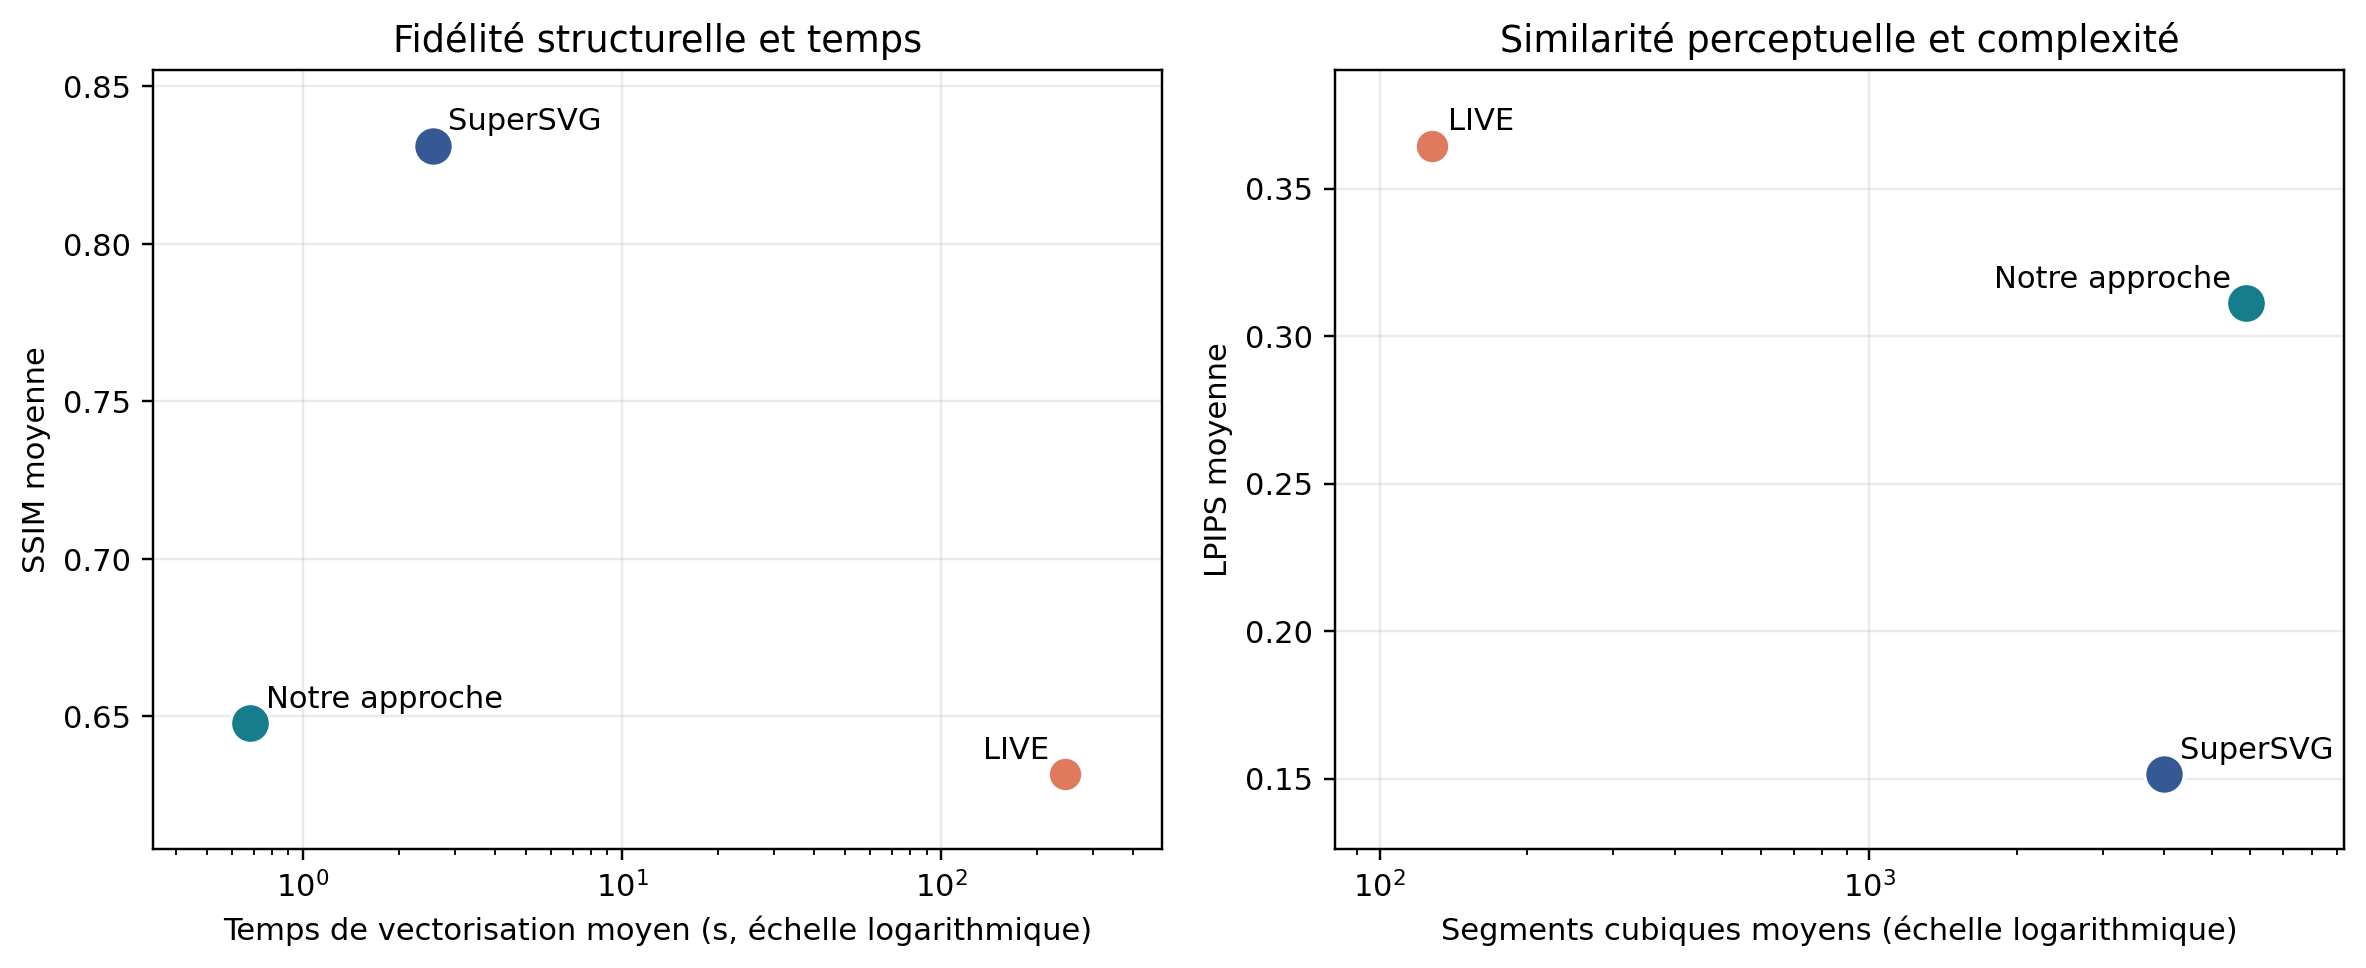
\includegraphics[width=\textwidth]{ch3_compromis_methodes.png}
    \caption{Compromis entre fidélité, temps de vectorisation et complexité des trois approches retenues pour l'analyse temporelle.}
    \label{fig:compromis_methodes}
\end{figure}

\subsection{Comparaison qualitative}

La figure~\ref{fig:comparaison_methodes_qualitative} présente les seize rendus utilisés pour les métriques. Sur la première image, SuperSVG restitue les deux animaux, le bâton et les transitions de couleur avec davantage de détails. Notre approche conserve la composition et les silhouettes principales, mais produit des aplats plus visibles. LIVE identifie les grandes régions, tout en simplifiant fortement les visages et l'arrière-plan en raison de son budget de $32$ chemins.

\begin{figure}[H]
    \centering
    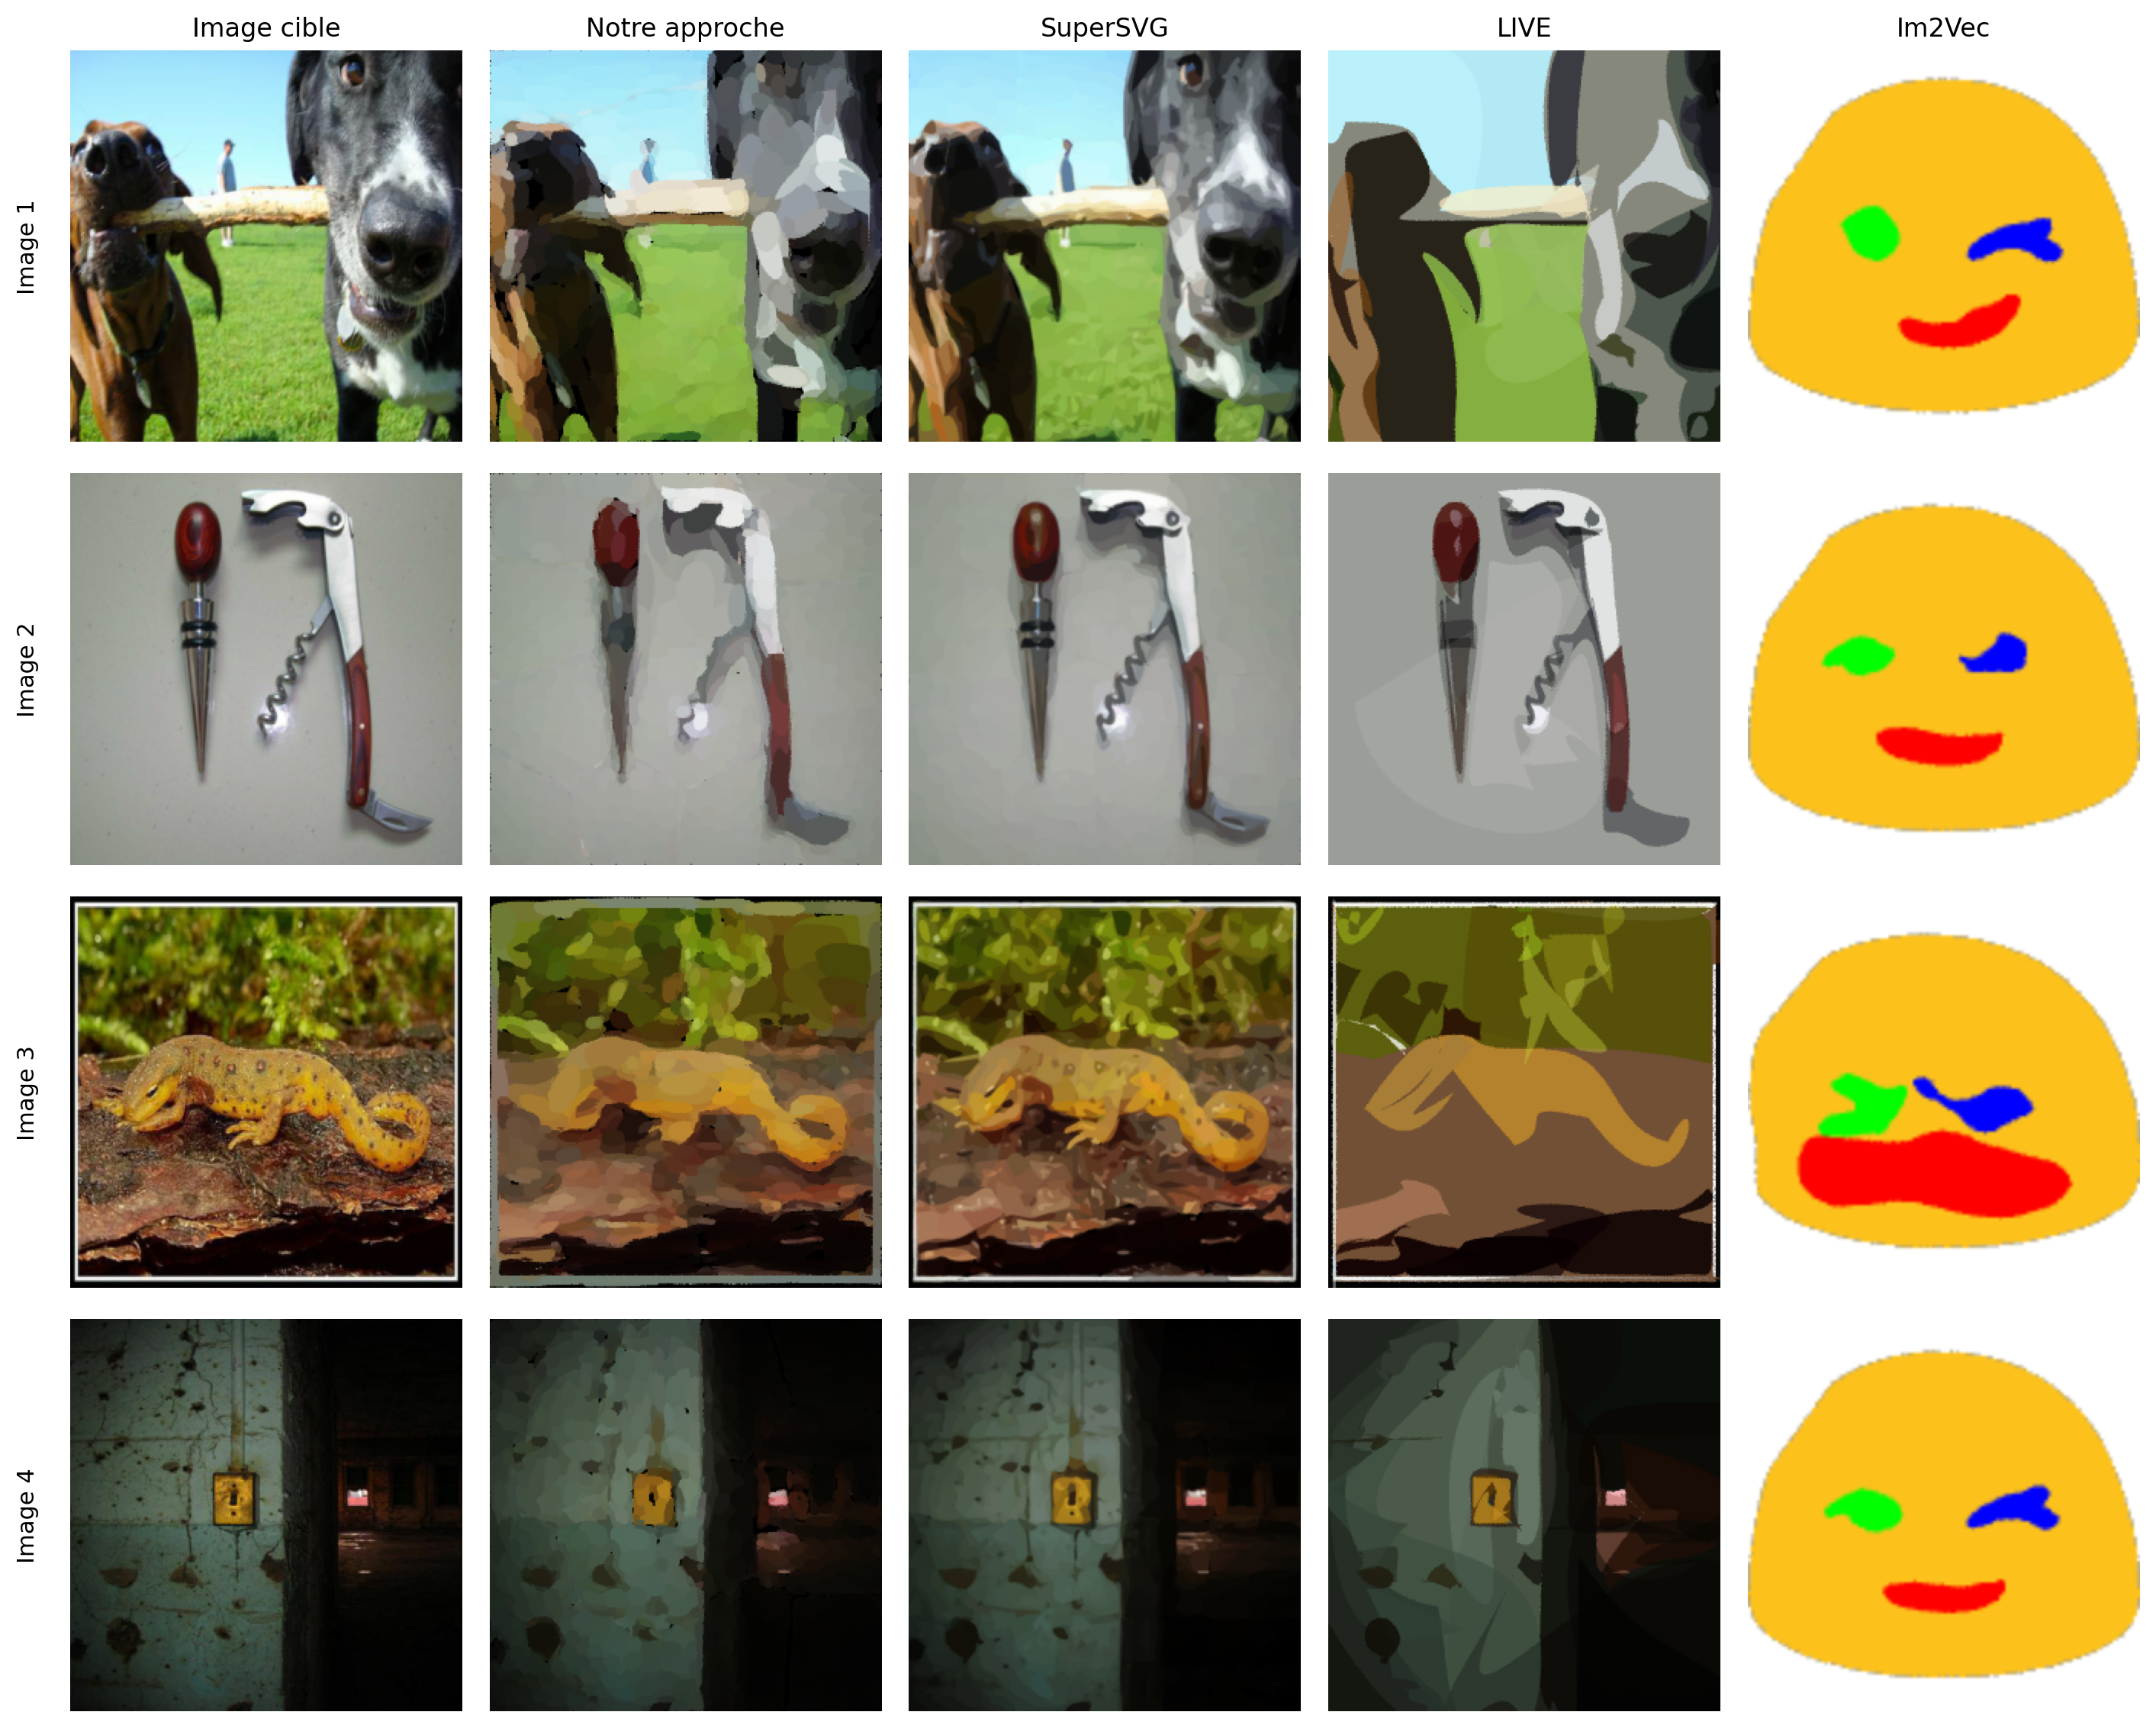
\includegraphics[width=\textwidth]{ch3_comparaison_methodes_qualitative.png}
    \caption{Comparaison qualitative des SVG rasterisés par la procédure commune.}
    \label{fig:comparaison_methodes_qualitative}
\end{figure}

La deuxième ligne constitue le cas le plus favorable aux trois approches directement adaptées aux images naturelles. Le fond uniforme et les contours distincts permettent à SuperSVG de reproduire les ustensiles avec précision. Notre approche et LIVE conservent leurs silhouettes, mais les petites courbes métalliques et les ombres deviennent moins précises. Sur la troisième image, la texture végétale et les taches de la salamandre sont difficiles à représenter par des surfaces opaques. SuperSVG préserve le mieux ces variations, notre modèle en fournit une approximation colorimétrique plus grossière et LIVE réduit la scène à un nombre limité de grandes formes.

Dans la scène sombre de la quatrième ligne, SuperSVG et notre approche conservent la séparation entre le mur, la porte et les petits éléments lumineux. LIVE respecte la structure globale avec moins de détails, ce qui explique une SSIM plus faible malgré une MSE proche. Les quatre sorties Im2Vec prennent au contraire la forme d'un visage stylisé composé de zones jaune, verte, bleue et rouge, ce qui correspond au décalage de domaine déjà signalé.

\subsection{Portée de la comparaison}

Le benchmark commun améliore la comparabilité par rapport à l'utilisation de valeurs publiées : les cibles, la machine, le rasteriseur et les métriques sont identiques. Il reste néanmoins limité à quatre images et à des configurations de capacités différentes. Notre approche utilise un nombre variable de chemins, SuperSVG reçoit une cible de $1\,000$ chemins et LIVE en optimise $32$. Im2Vec, qui n'en génère que quatre et ne reconstruit pas suffisamment les photographies, est exclu de l'analyse temporelle. Les résolutions internes, les domaines et les budgets d'entraînement diffèrent également, puisque nous évaluons les checkpoints disponibles sans réentraînement commun.

Ces résultats ne constituent donc pas un classement général des architectures. Ils décrivent le comportement des implémentations et des checkpoints disponibles sur un petit ensemble commun de photographies naturelles. Une comparaison contrôlée supplémentaire demanderait de réentraîner les modèles sur les mêmes données, d'imposer plusieurs budgets de segments identiques et d'élargir le jeu de test. Malgré cette réserve, l'expérience fournit une référence externe concrète qui complète l'étude interne de notre architecture.

\section{Étude interne des configurations proposées}
\label{sec:resultats_quantitatifs}

Après la comparaison externe, nous examinons plus précisément les deux configurations issues de notre entraînement. Cette étude met en relation leur fidélité de reconstruction avec le temps d'inférence et la complexité des documents SVG produits.

\subsection{Fidélité de reconstruction}

Le tableau~\ref{tab:resultats_fidelite} compare les deux configurations finales. Le modèle à $128$ chemins obtient la meilleure moyenne pour chacune des quatre métriques. La MSE passe de $0{,}01615$ à $0{,}00573$, soit une diminution absolue favorable de $0{,}01042$, et le PSNR gagne $5{,}00$ dB. La SSIM passe de $0{,}438$ à $0{,}645$, soit une augmentation de $0{,}207$, tandis que la LPIPS diminue de $0{,}492$ à $0{,}290$, soit un écart favorable de $0{,}202$. L'amélioration concerne ainsi les mesures pixel par pixel, structurelles et perceptuelles.

\begin{table}[H]
    \centering
    \small
    \caption{Résultats moyens de fidélité sur les 12 images du jeu de test.}
    \label{tab:resultats_fidelite}
    \begin{tabular}{lcccc}
        \toprule
        \textbf{Configuration} & \textbf{MSE $\downarrow$} & \textbf{PSNR $\uparrow$} & \textbf{SSIM $\uparrow$} & \textbf{LPIPS $\downarrow$} \\
        \midrule
        $32$ chemins  & $0{,}01615 \pm 0{,}01181$ & $19{,}13 \pm 3{,}54$ & $0{,}438 \pm 0{,}152$ & $0{,}492 \pm 0{,}058$ \\
        $128$ chemins & $\mathbf{0{,}00573 \pm 0{,}00533}$ & $\mathbf{24{,}13 \pm 4{,}05}$ & $\mathbf{0{,}645 \pm 0{,}135}$ & $\mathbf{0{,}290 \pm 0{,}075}$ \\
        \bottomrule
    \end{tabular}
\end{table}

L'amélioration est observée sur les $12$ images pour la MSE, la SSIM et la LPIPS, et non uniquement sur la moyenne. La figure~\ref{fig:comparaison_quantitative} présente les moyennes et les écarts-types. La dispersion reste importante pour la MSE et le PSNR, car la difficulté varie fortement entre une scène texturée contenant plusieurs objets et une image sombre dominée par de grandes zones uniformes.

\begin{figure}[H]
    \centering
    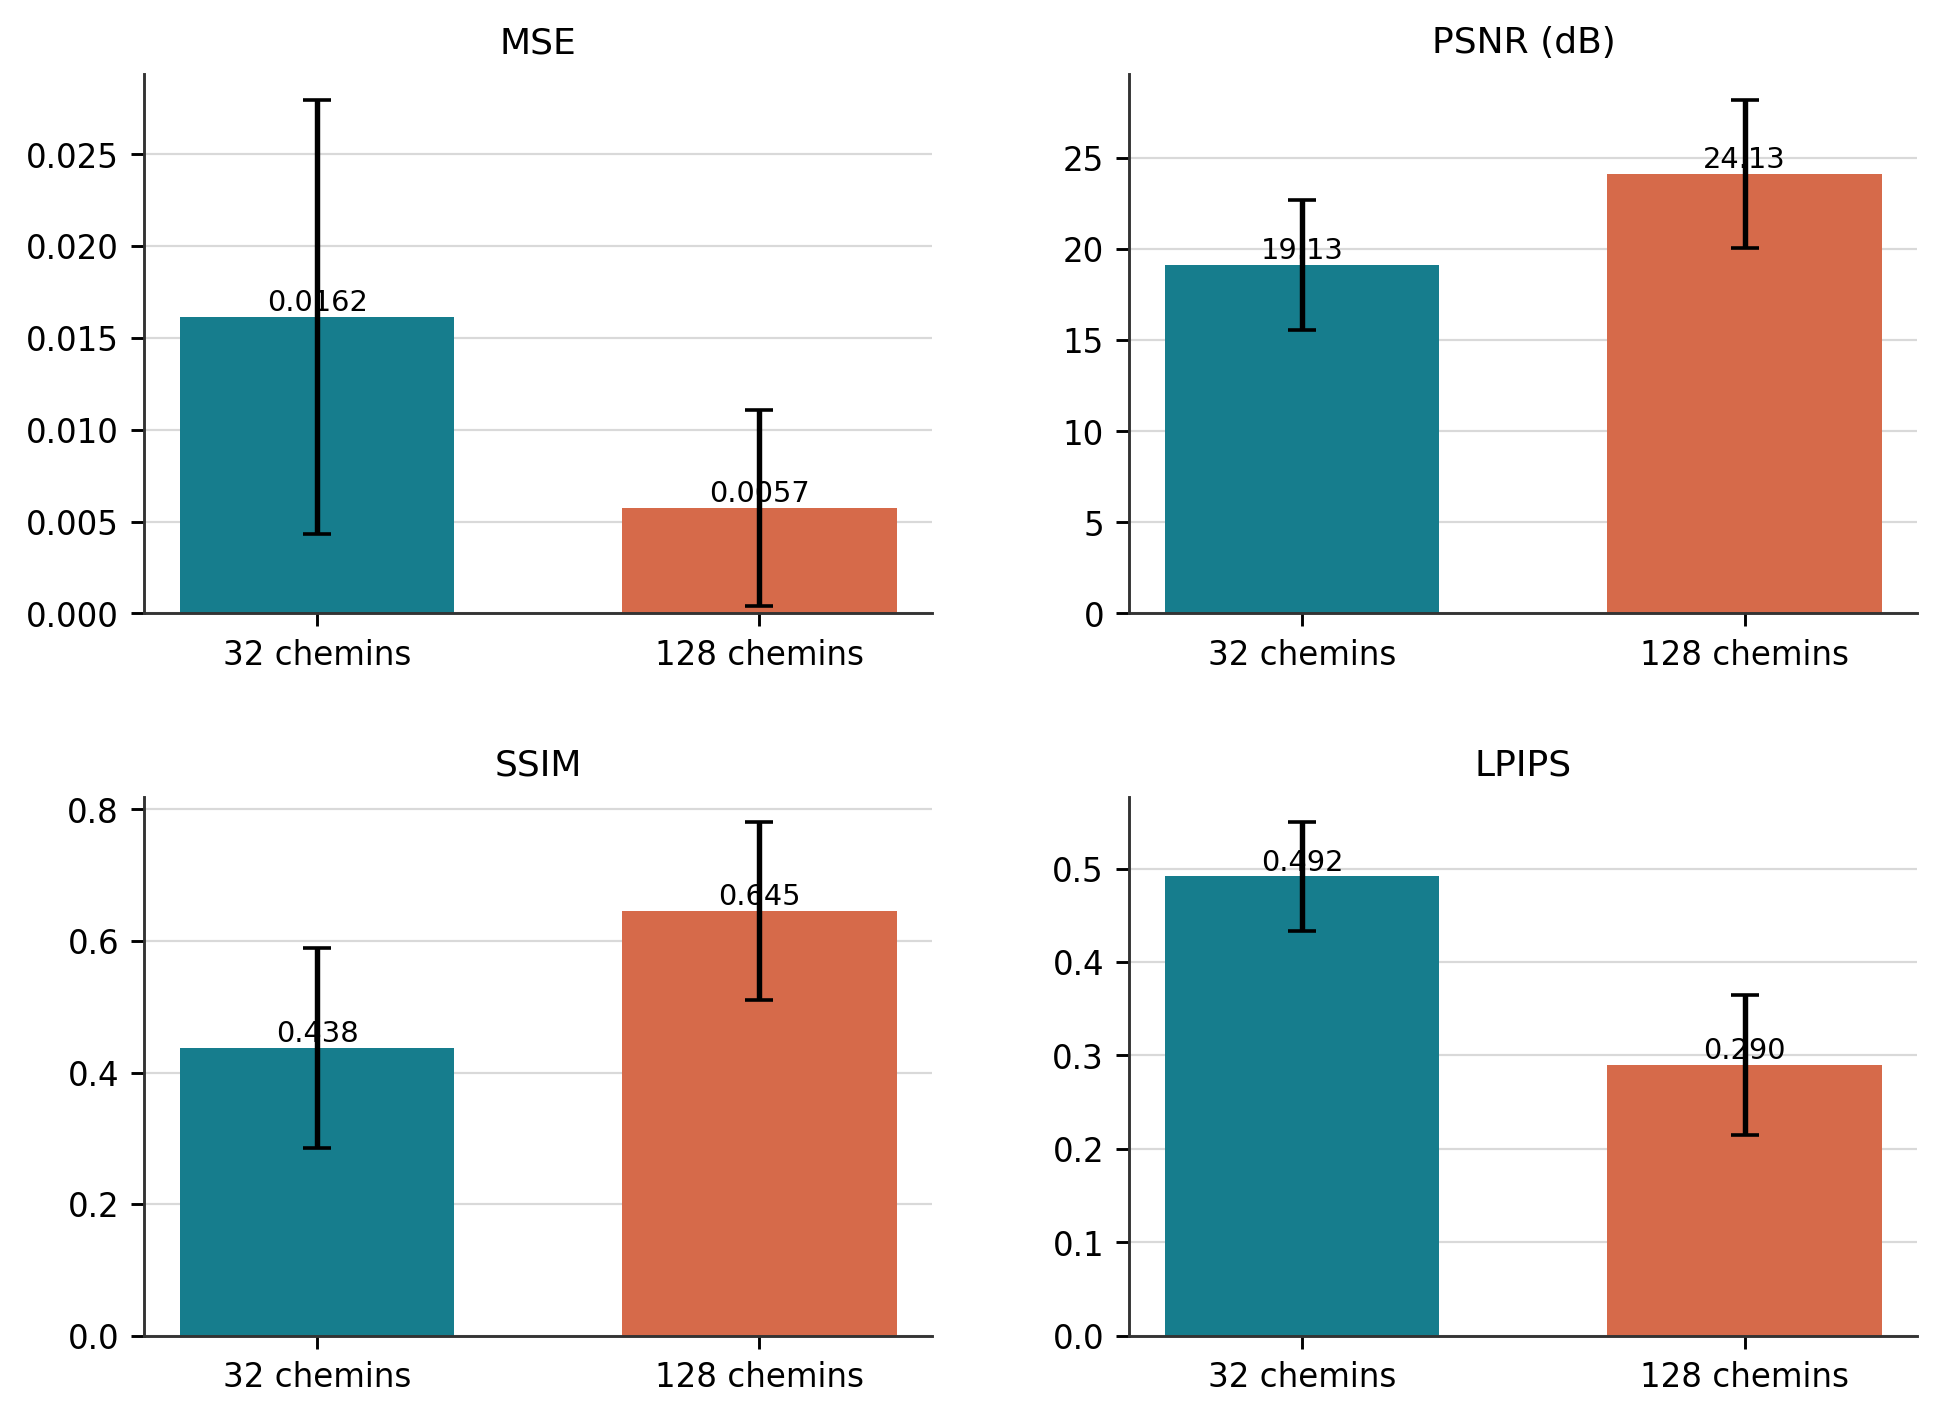
\includegraphics[width=0.92\textwidth]{ch3_comparaison_quantitative.png}
    \caption{Comparaison quantitative des configurations finales; les barres d'erreur représentent l'écart-type.}
    \label{fig:comparaison_quantitative}
\end{figure}

La meilleure valeur de SSIM du modèle à $128$ chemins, égale à $0{,}848$, est obtenue sur l'image contenant les deux ustensiles placés sur un fond relativement uniforme. Le PSNR maximal atteint $29{,}83$ dB sur une scène sombre dont de larges régions sont peu texturées. À l'inverse, l'image de la salamandre entourée d'une végétation détaillée obtient une SSIM de $0{,}465$, malgré l'augmentation du nombre de chemins. Ces écarts montrent que les formes principales et les aplats de couleur sont plus faciles à approximer que les petites variations répétées de texture.

Compte tenu des budgets précisés dans le tableau~\ref{tab:configurations_evaluees}, ces écarts portent sur les deux configurations complètes et ne permettent pas d'isoler l'effet du seul nombre de primitives.

\subsection{Temps d'inférence et complexité du SVG}

L'augmentation de la fidélité s'accompagne d'un coût vectoriel. Le tableau~\ref{tab:cout_inference_svg} détaille les temps moyens. La préparation SLIC et le passage dans le réseau restent presque constants. En revanche, le rendu passe de $0{,}155$ à $0{,}475$ seconde et l'export de $0{,}040$ à $0{,}141$ seconde. Le temps total mesuré est ainsi multiplié par $2{,}67$.

\begin{table}[H]
    \centering
    \footnotesize
    \caption{Coût moyen de l'inférence et complexité des SVG générés.}
    \label{tab:cout_inference_svg}
    \begin{tabular}{p{4.2cm}p{4.0cm}p{4.0cm}}
        \toprule
        \textbf{Mesure} & \textbf{32 chemins} & \textbf{128 chemins} \\
        \midrule
        Préparation des régions (s) & $0{,}0366 \pm 0{,}0044$ & $0{,}0349 \pm 0{,}0039$ \\
        Passage dans le réseau (s) & $0{,}0208 \pm 0{,}0020$ & $0{,}0206 \pm 0{,}0019$ \\
        Rendu DiffVG (s) & $0{,}1547 \pm 0{,}0312$ & $0{,}4752 \pm 0{,}0933$ \\
        Export SVG (s) & $0{,}0398 \pm 0{,}0303$ & $0{,}1408 \pm 0{,}0633$ \\
        Temps total mesuré (s) & $0{,}2520 \pm 0{,}0483$ & $0{,}6715 \pm 0{,}1361$ \\
        Mémoire GPU supplémentaire (Mo) & $80{,}1 \pm 7{,}5$ & $80{,}9 \pm 6{,}3$ \\
        Nombre de chemins & $354{,}7 \pm 76{,}5$ & $1\,418{,}7 \pm 306{,}1$ \\
        Taille du SVG (Ko) & $158{,}9 \pm 34{,}2$ & $633{,}4 \pm 136{,}9$ \\
        \bottomrule
    \end{tabular}
\end{table}

Le nombre de chemins et la taille du fichier sont presque exactement multipliés par quatre, car les deux configurations utilisent les mêmes régions et sérialisent respectivement $32$ et $128$ primitives pour chacune. La mémoire GPU supplémentaire reste proche de $81$ Mo. Ce résultat s'explique par le fait que le backbone domine le nombre de paramètres et que les scènes DiffVG sont rendues par image. Le principal coût de la configuration à $128$ chemins est donc temporel et documentaire, plutôt que lié à une forte augmentation de la mémoire du réseau.

La figure~\ref{fig:cout_vectorisation} visualise ce compromis. DiffVG et l'export représentent la majorité du temps, surtout pour le modèle à $128$ chemins. Une réduction de la complexité après la prédiction, par exemple par suppression des chemins redondants ou fusion de formes proches, pourrait donc diminuer à la fois le temps de sérialisation, la taille du fichier et la difficulté d'édition.

\begin{figure}[H]
    \centering
    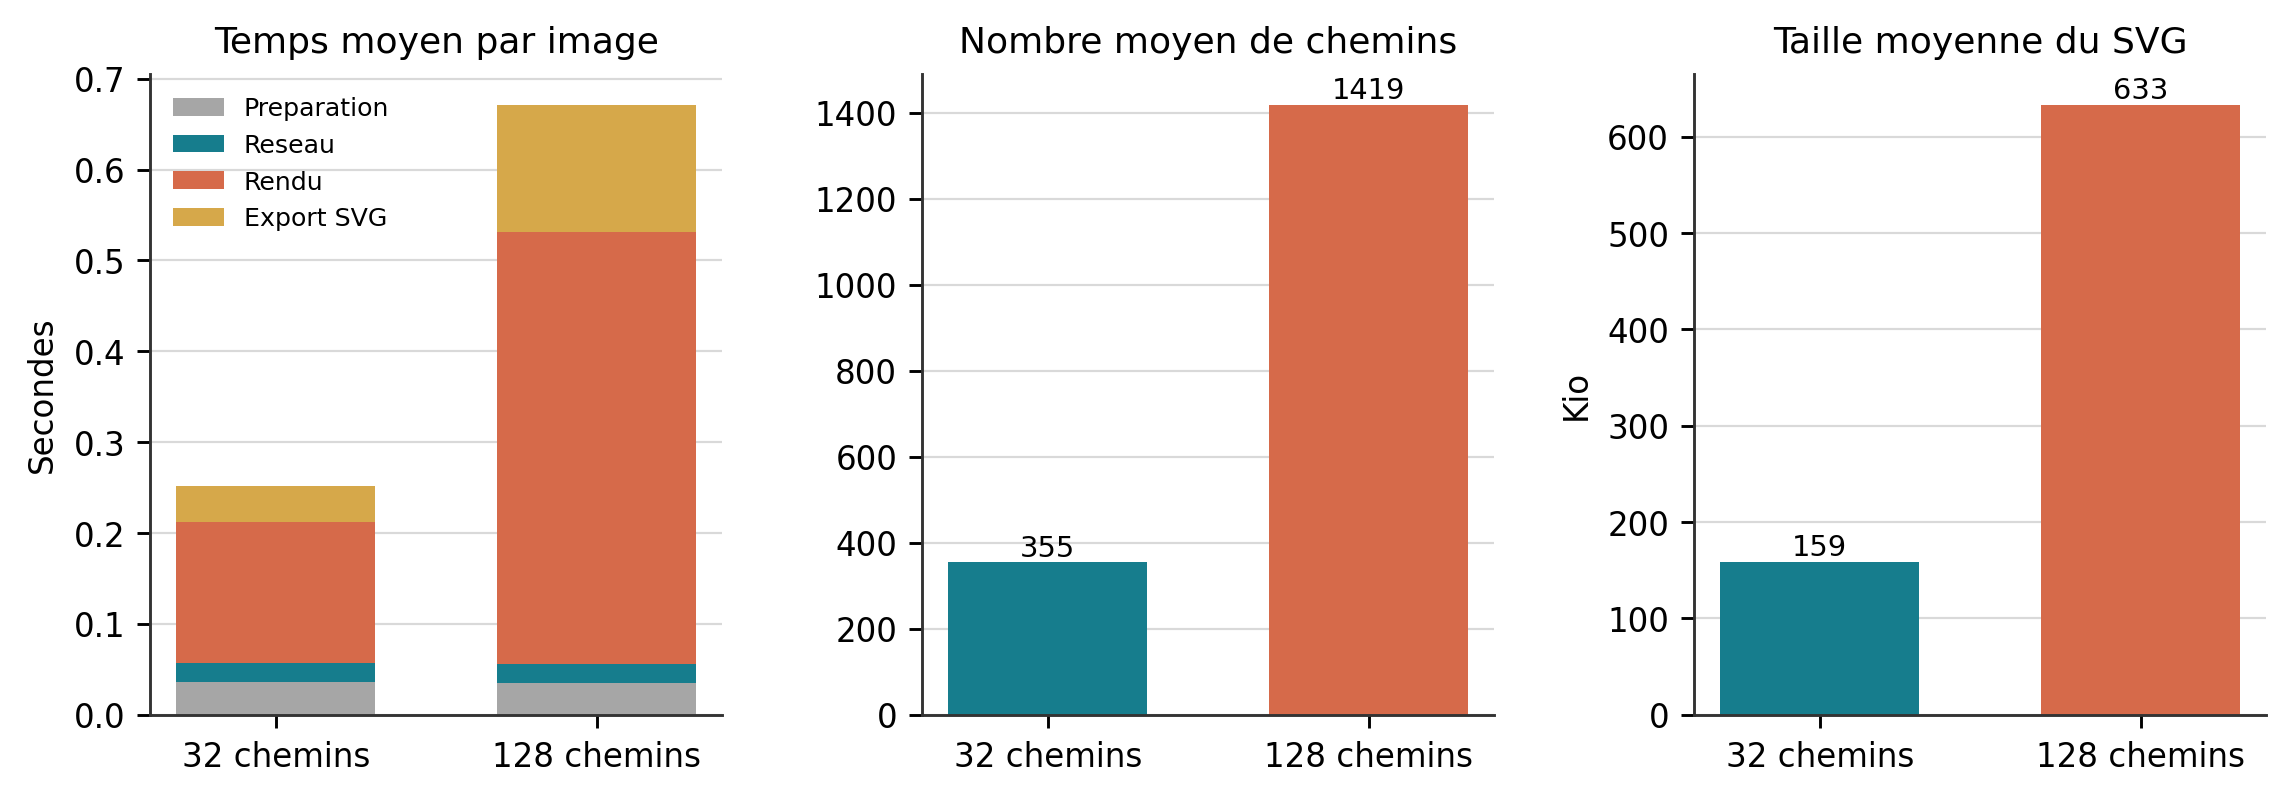
\includegraphics[width=\textwidth]{ch3_cout_vectorisation.png}
    \caption{Répartition du temps moyen et évolution de la complexité vectorielle.}
    \label{fig:cout_vectorisation}
\end{figure}

\section{Analyse qualitative de l'approche proposée}
\label{sec:resultats_qualitatifs}

La figure~\ref{fig:comparaison_qualitative} présente trois exemples choisis pour illustrer des comportements différents. Elle compare l'image matricielle, le rendu du modèle à $32$ chemins et celui du modèle à $128$ chemins. Les valeurs indiquées sous les reconstructions correspondent aux métriques propres à chaque image.

\begin{figure}[H]
    \centering
    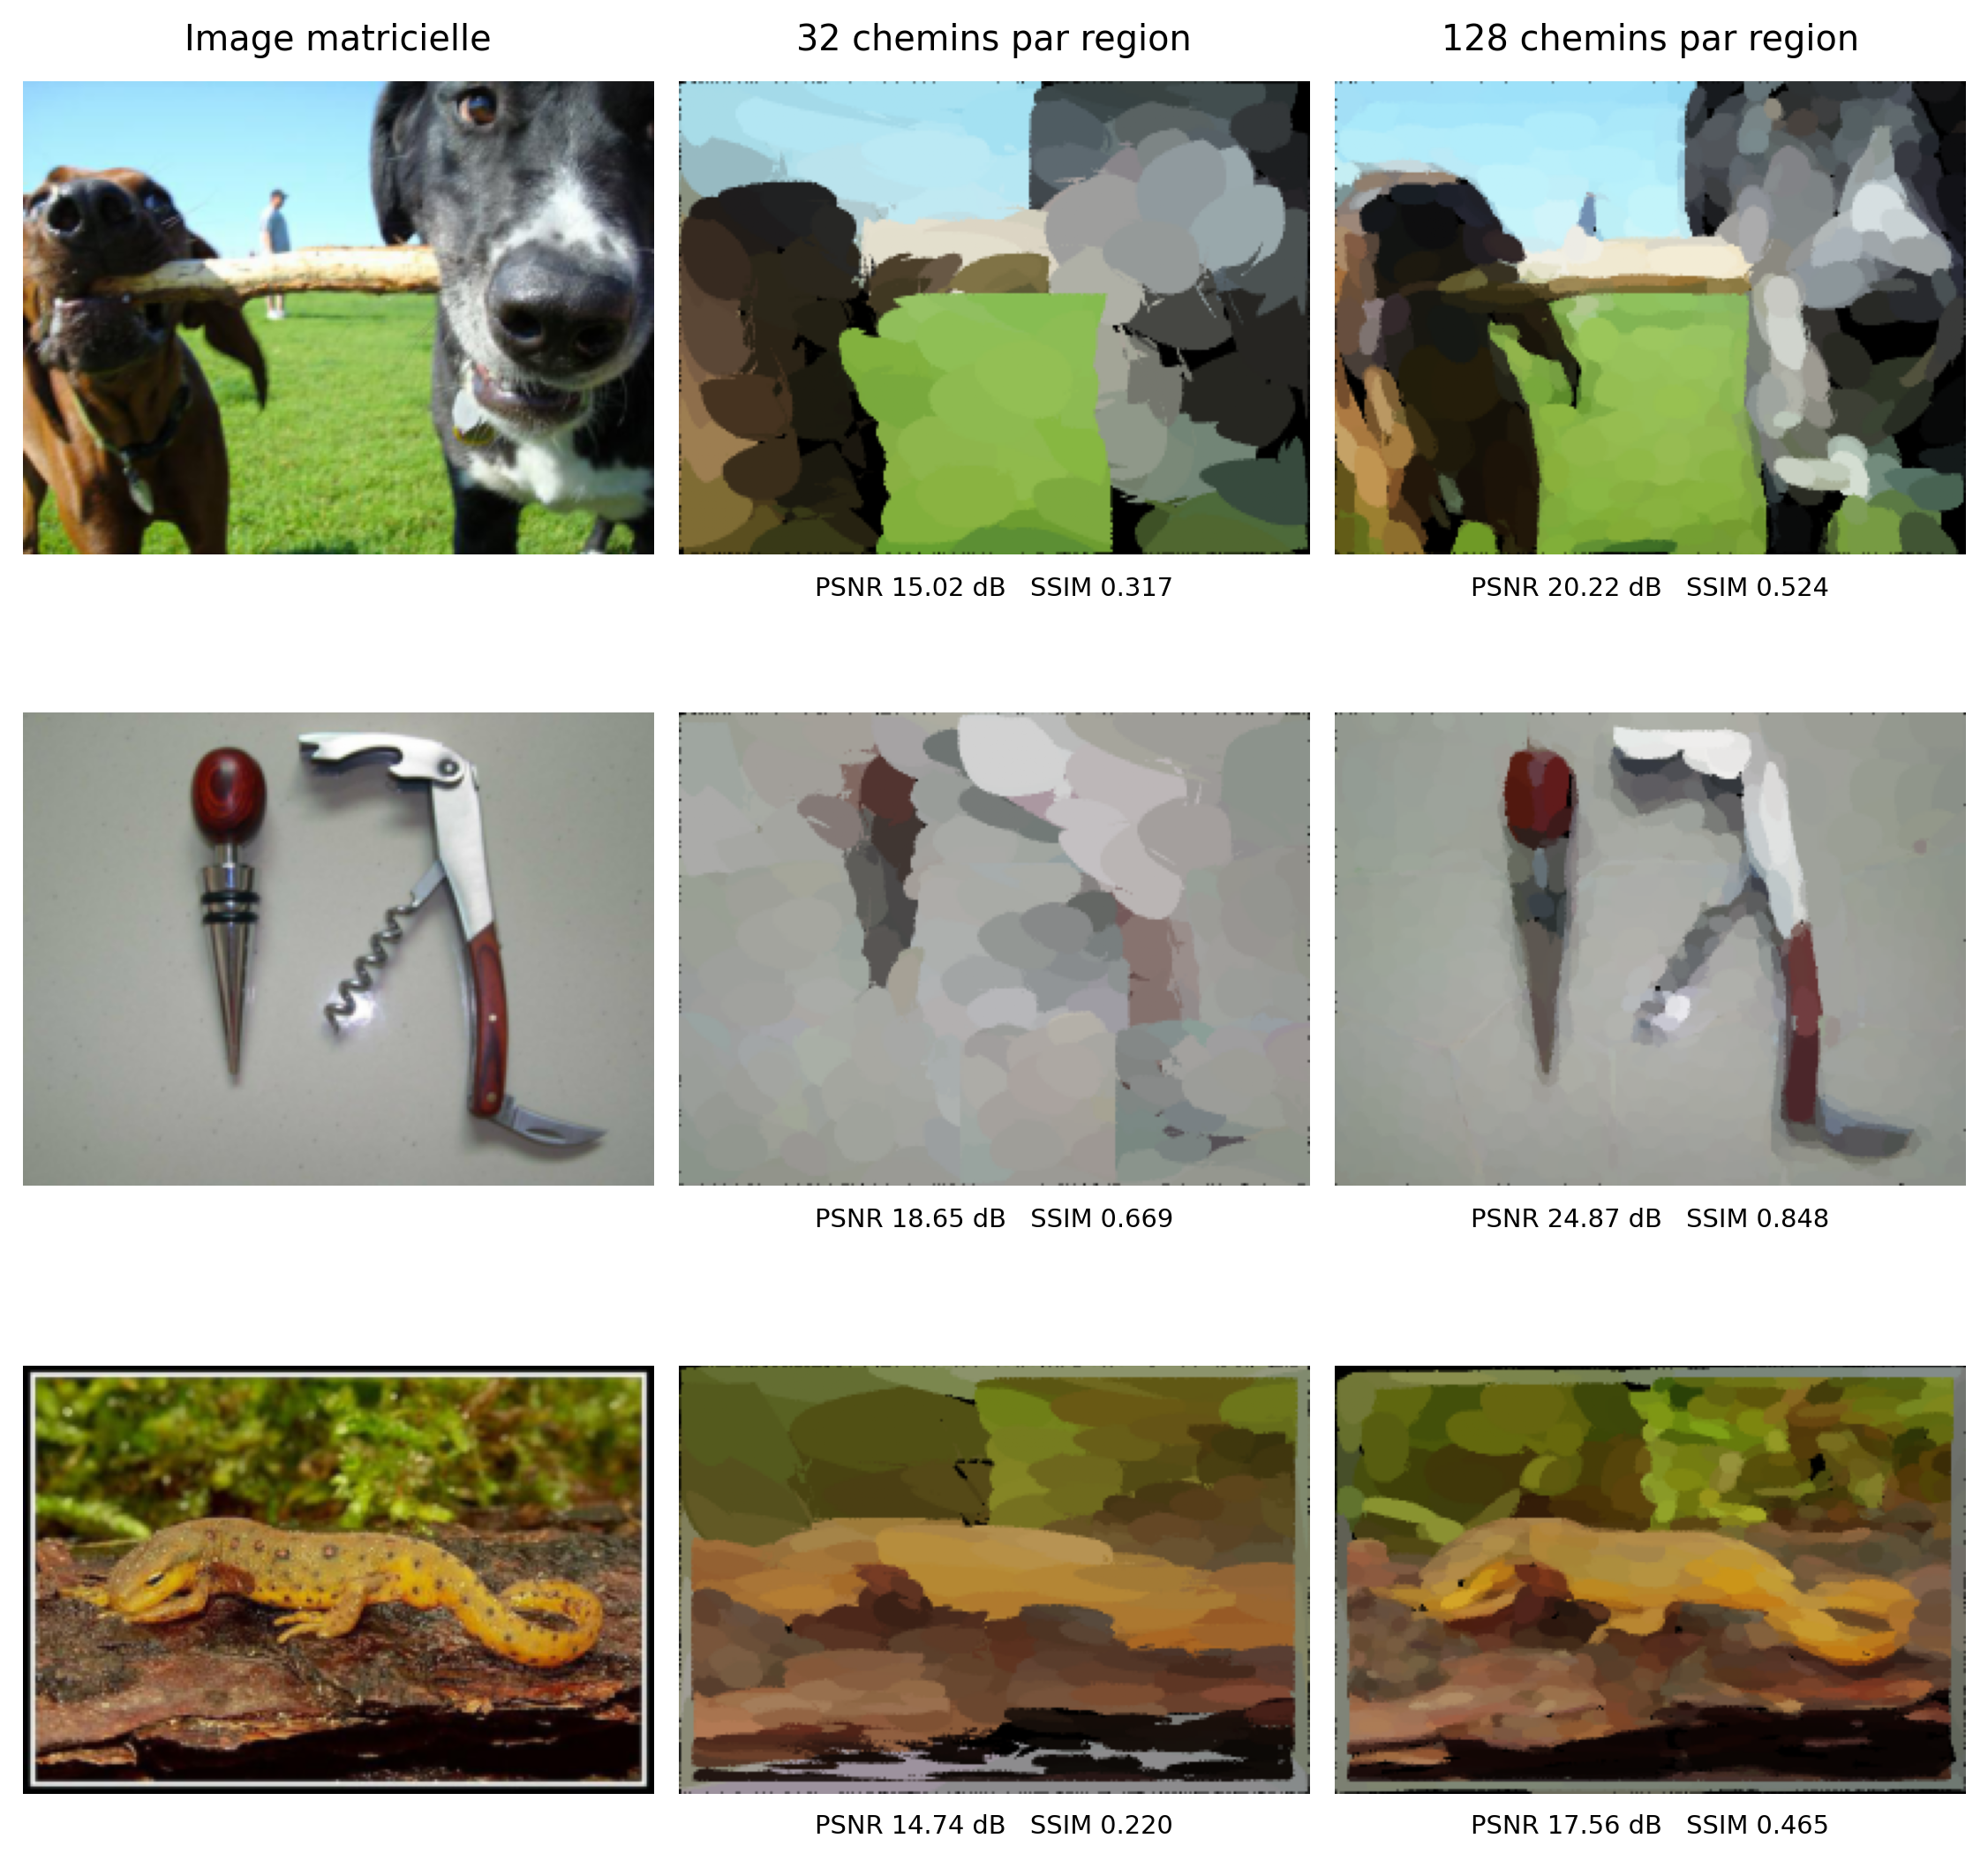
\includegraphics[width=\textwidth]{ch3_comparaison_qualitative.png}
    \caption{Comparaison qualitative sur une scène complexe, un objet isolé et une image fortement texturée.}
    \label{fig:comparaison_qualitative}
\end{figure}

Dans la première ligne, la configuration à $32$ chemins reconstruit les principales masses de couleur, notamment le ciel, l'herbe et les deux animaux, mais plusieurs détails du visage sont confondus. Avec $128$ chemins, les yeux, les museaux, le bâton et les transitions de couleur deviennent plus reconnaissables. Le PSNR passe de $15{,}02$ à $20{,}22$ dB, soit un gain de $5{,}20$ dB, et la SSIM de $0{,}317$ à $0{,}524$, soit une augmentation absolue de $0{,}207$. La reconstruction reste cependant stylisée et composée d'aplats superposés plutôt que de textures proches de la photographie.

La deuxième ligne montre un cas plus favorable. Le fond est presque uniforme et les objets possèdent des silhouettes distinctes. La configuration à $32$ chemins restitue mal les deux ustensiles, car une partie importante des primitives est utilisée pour approximer le fond et les ombres. Le modèle à $128$ chemins sépare clairement les deux objets, retrouve leurs couleurs dominantes et conserve la forme générale du tire-bouchon. La SSIM atteint alors $0{,}848$.

La troisième ligne contient une salamandre sur un arrière-plan riche en mousse et en bois. Le modèle à $128$ chemins améliore la silhouette et la répartition des couleurs, mais ne reproduit pas les petites taches ni les variations fines de la végétation. Le résultat à $32$ chemins réduit l'animal à une forme allongée et plusieurs zones du fond fusionnent. Cet exemple confirme que l'augmentation du nombre de primitives aide à représenter les détails, mais ne résout pas entièrement la perte d'information provoquée par la segmentation locale et par la représentation en surfaces opaques.

Plusieurs artefacts sont communs aux résultats. De minces zones noires peuvent apparaître lorsque les formes ne couvrent pas complètement une frontière, tandis que des superpositions produisent parfois une transition abrupte entre régions. Les chemins étant fermés, sans contour et sans transparence, le modèle doit représenter toutes les variations par des aplats colorés. Enfin, les frontières de SLIC restent visibles dans certaines reconstructions, car les régions sont prédites indépendamment puis concaténées sans étape globale de raccordement.

Sur le plan de l'éditabilité, tous les fichiers sont de véritables SVG composés de chemins de Bézier et peuvent être ouverts par DiffVG. Néanmoins, un document contenant en moyenne plus de $1\,400$ chemins devient difficile à modifier manuellement. La configuration à $32$ chemins est plus compacte, mais sa simplification visuelle est nettement plus forte. La qualité d'une approche de vectorisation ne doit donc pas être jugée uniquement par la similarité matricielle : le nombre et l'organisation des primitives restent déterminants.

\section{Discussion et limites}
\label{sec:discussion_limites_resultats}

Les résultats montrent que le réseau produit en une seule passe des primitives conduisant à des SVG valides, tandis que les métriques évoluent favorablement au cours de l'apprentissage. Dans le benchmark externe, SuperSVG offre la meilleure fidélité, notre approche occupe une position intermédiaire entre vitesse et qualité, et LIVE privilégie la compacité au prix d'une optimisation beaucoup plus longue. L'étude interne met également en évidence un compromis : la configuration à $128$ chemins améliore la reconstruction, mais augmente le temps de rendu et la complexité documentaire.

Ces constats restent circonscrits aux conditions définies dans la section~\ref{sec:comparaison_methodes}. Le nombre réduit d'images, l'hétérogénéité des configurations disponibles, l'exécution temporelle unique par image et l'absence de vérité terrain SVG empêchent d'en déduire un classement général. Les mesures caractérisent la fidélité matricielle, le coût et la structure des fichiers produits dans notre environnement; elles n'évaluent pas directement leur proximité avec un document conçu par un graphiste.

Sur le plan architectural, le nombre de chemins fixe par superpixel entraîne des primitives redondantes dans les régions simples, tandis que le traitement indépendant des régions peut créer des discontinuités. Les surfaces opaques sans traits ni dégradés limitent en outre la représentation des textures fines. Une capacité adaptative, une simplification des chemins après prédiction et un raffinement global \textit{coarse-to-fine} constituent ainsi des prolongements cohérents. Des expériences contrôlées avec des budgets d'entraînement identiques seraient nécessaires pour isoler l'effet du nombre de chemins, de l'ajustement du backbone DINOv3 et des paramètres SLIC.

\section{Conclusion}

Dans ce chapitre, nous avons vérifié la chaîne de rendu différentiable et la validité des SVG, puis évalué notre architecture selon deux niveaux complémentaires. La comparaison externe place SuperSVG en tête pour la fidélité, tandis que notre approche réduit le temps de vectorisation au prix d'un plus grand nombre de primitives; LIVE produit des documents plus compacts mais nécessite une optimisation sensiblement plus longue.

L'étude interne montre que la configuration à $128$ chemins améliore les quatre métriques par rapport à celle à $32$ chemins, avec un coût supérieur en temps de rendu et en complexité du SVG. Ces observations soutiennent la faisabilité de la prédiction directe de primitives à partir du backbone DINOv3, tout en orientant la suite du travail vers un raffinement visuel et une capacité vectorielle plus adaptative.



% ============================================================
%   CONCLUSION GÉNÉRALE
% ============================================================
\chapter*{Conclusion Générale}
\addcontentsline{toc}{chapter}{Conclusion Générale}
\markboth{Conclusion Générale}{Conclusion Générale}

Ce projet de fin d'études a porté sur la vectorisation automatique d'images matricielles par
apprentissage profond. Nous avons conçu une chaîne qui segmente l'image avec SLIC, extrait
les caractéristiques des régions avec DINOv3 et prédit, par attention, des chemins fermés de
Bézier et leur couleur. DiffVG permet d'entraîner ce modèle sans disposer de SVG de référence.

Les tests ont confirmé la transmission des gradients et la validité des $24$ SVG contrôlés. Sur
les $12$ images internes, la configuration à $128$ chemins par superpixel obtient une MSE de
$0{,}00573$, un PSNR de $24{,}13$ dB, une SSIM de $0{,}645$ et une LPIPS de $0{,}290$.
Sur les quatre images du benchmark externe, SuperSVG présente la meilleure fidélité moyenne, notre approche atteint
un temps de vectorisation moyen de $0{,}684$ seconde et LIVE produit les fichiers les plus
compacts.

Les perspectives concernent d'abord l'adaptation du nombre de chemins, la simplification des
primitives et l'ajout d'un raffinement global \textit{coarse-to-fine}. Les paramètres de SLIC,
notamment le nombre de régions et la compacité, pourraient également être prédits selon le
contenu de l'image ou intégrés à une formulation apprenable. Une autre possibilité consiste à
employer des métaheuristiques, comme un algorithme génétique, pour sélectionner conjointement
ces paramètres, le nombre de chemins et les poids des pertes selon un compromis entre fidélité
et complexité. Enfin, un benchmark plus étendu et des entraînements contrôlés permettraient
de confirmer les résultats.
Le système développé constitue ainsi une base fonctionnelle pour ces améliorations.

% ============================================================
%   BIBLIOGRAPHIE
% ============================================================
\printbibliography[heading=bibintoc, title={Bibliographie}]

% ============================================================
%   ANNEXES  (optionnel)
% ============================================================
% \appendix
% \chapter{Titre de l'annexe A}
% \lipsum[1]

\end{document}
